\documentclass[oneside,a4paper,11pt,openrany]{book}

%openright

\usepackage{ThesisStyle}
% \usepackage{apacite}	% - For the bibliography
\usepackage[square,numbers]{natbib}
\usepackage{comment}
\usepackage[usenames]{color}
\usepackage[spanish, es-tabla]{babel}
\usepackage{pdfpages}
\usepackage[utf8]{inputenc}
\usepackage{listings}
\usepackage{soul}
\usepackage{soulutf8}

\setboolean{@twoside}{true}	% - Setting twoside boolean to true (does not change margin)


\title{Ecosistema para el Descubrimiento de Conocimiento en Lenguaje Natural} % - Thesis name

\begin{document}

%%TC:ignore

	%	<Cover>	%
	%\include{./Chapters/Cover/Cover}
	\begin{titlepage}

\center % Center everything on the page


%----------------------------------------------------------------------------------------
%	LOGO SECTION
%----------------------------------------------------------------------------------------


\includegraphics[scale=.60]{./Images//Chapters/Cover/UA.jpg}\\[.5cm] % Include a department/university logo - this will require the graphicx package



%----------------------------------------------------------------------------------------
%	HEADING SECTIONS
%----------------------------------------------------------------------------------------
{\Large Departamento de Lenguajes y Sistemas Inform{\'a}ticos}\\[0.25cm] % Department
{\Large Escuela Polit{\'e}cnica Superior}\\[2.0cm] % University

%----------------------------------------------------------------------------------------
%	TITLE SECTION
%----------------------------------------------------------------------------------------

%\HRule \\[0.4cm]
{ \huge \bfseries Ecosistema para el}\\[0.3cm]
{ \huge \bfseries Descubrimiento de Conocimiento}\\[0.3cm]
{ \huge \bfseries en Lenguaje Natural}\\[1.5cm] % Thesis title
%\HRule \\[1.5cm]
 
%----------------------------------------------------------------------------------------
%	AUTHOR SECTION
%----------------------------------------------------------------------------------------

{ \LARGE Alejandro Piad Morffis}\\[1.5cm]


%----------------------------------------------------------------------------------------
%	PROGRAM SECTION
%----------------------------------------------------------------------------------------

{ \it Tesis presentada para aspirar al grado de }\\[.25cm]
{ DOCTOR POR LA UNIVERSIDAD DE ALICANTE }\\[.25cm]
{ MENCI{\'O}N DE DOCTOR INTERNACIONAL }\\[.25cm]
{ DOCTORADO EN INFORM{\'A}TICA }\\[0.5cm]


%----------------------------------------------------------------------------------------
%	SUPERVISION SECTION
%----------------------------------------------------------------------------------------

{ \it Dirigida por }\\[.25cm]
{ Dr. Yoan Gutierrez Vazquez \\ Dr. Yudivian Almeida Cruz \\ Dr. Rafael Muñoz Guillena }\\[1.5cm]


%----------------------------------------------------------------------------------------
%	FUNDING SECTION
%----------------------------------------------------------------------------------------

{ Esta tesis ha sido co-dirigida y financiada por\\la Universidad de Alicante y la Universidad de La Habana. }


%----------------------------------------------------------------------------------------

\vfill % Fill the rest of the page with whitespace

\end{titlepage}

	\blankpage
	{
\center

\Large{\bf TESIS DOCTORAL EN FORMA DE COMPENDIO DE PUBLICACIONES} 
\BlankLine

Ecosistema para el Descubrimiento de Conocimiento en Lenguaje Natural
\BlankLine
}

El presente documento contiene una síntesis del trabajo realizado por Alejandro Piad Morffis, bajo la dirección de Dr. Yoan Gutierrez Vazquez, Dr. Rafael Muñoz Guillena y Dr. Yudivián Almeida Cruz, para optar por el grado de Doctor en Informática. Se presenta en la Universidad de Alicante y se estructura según
la normativa establecida para la presentación de tesis doctorales en forma de compendio de publicaciones: una primera parte con una síntesis, una segunda parte que reproduce las publicaciones científicas realizadas y una tercera parte con las conclusiones.

	\blankpage

	%	<Dedication>	%
	\thispagestyle{empty}

\vspace*{\fill}

\begin{flushright}
\textit{A mi familia y amigos, por hacerme quien soy.}

\textit{A Sue, por enseñarme a querer más.}

\textit{A papá, por creer.}
\end{flushright}

\vspace*{\fill}
	%	- Dedication

	%\frontmatter
	\pagestyle{fancyUnnumberedSectionsStyle}	% - Fixing style for the regular chapters
	\chapter*{Agradecimientos}
\markboth{Agradecimientos}{}
\phantomsection
\pagenumbering{roman}

Cuando empecé la aventura que me traje al día de hoy, allá por el año 2008, yo tenía grandes expectativas pero ningún plan concreto.
Sabía que quería estudiar en la Universidad de La Habana, y que quería hacer algo con computadoras, pero nada más.
Mi padre se sentó conmigo, él al timón, yo en el asiento del acompañante, como siempre hacíamos por esa época, esperando a que mi hermana, quien entonces estudiaba violín, terminara sus clases.

Papá me preguntó cuáles eran mis aspiraciones ahora que comenzaba la Universidad.
Él siempre recordaba la Universidad como la época de su vida donde más grande se hizo su mundo, y creo que por eso quería que la mía fuera una experiencia excepcional.
Yo le dije simplemente que quería ser el mejor. El mejor de mi clase, el mejor de toda la carrera, vaya, el mejor del mundo incluso.
Y en vez de decirme cuan ridículas eran esas expectativas, me dijo ``pues hagamos un plan para lograr eso''.

Y así lo hicimos, planeamos ahí en media hora los pasos que supuestamente me iban a llevar a cumplir esas ridículas metas. Pasos que tenían que ver con dedicar no se cuántas horas a estudiar, con hacerme alumno ayudante lo antes posible, con trabajar en proyectos adicionales.
Hoy sé que no había ninguna garantía de que esos pasos me llevaran a ser el mejor del mundo, pero al menos me trajeron hasta aquí.
Y así aprendí que los sueños no están para cumplirse, están para empujarte a llegar más lejos, mucho más lejos de lo que tu pudieras imaginar, aunque muchas veces en direcciones totalmente diferentes de las que soñaste.

Este sueño lo he compartido con muchísimas personas, tantas que me es imposible agradecerles a todos por las huellas que han dejado en mi vida. Trataré de mencionar a algunos de los imprescindibles, pero pido disculpas de antemano por todos aquellos que seguro me faltarán.

En primer lugar, tengo que agradecer infinitamente a mi padre. Agradecerle por muchas cosas simples y mundanas, como enseñarme a montar bicicleta, a nadar, a disfrutar de los libros, a conducir, a comer saludable, a querer a los demás por sus defectos y no a pesar de ellos, y a soñar en grande.
Pero lo más importante que me dió mi padre no fueron ni habilidades específicas ni su filosofía de vida.
Papá siempre creyó que yo podía lograr lo que me propusiera, incluso cuando eso no coincidiera con lo que él veía más importante o valioso, incluso aunque que mis planes y expectativas me llevaran lejos de las suyas.
Y no es cierto, uno no puede lograr todo lo que se propone, claro que no.
Su propia vida estuvo llena de metas fallidas y expectativas frustradas, como la de todos.
Pero si uno no cree que puede, no tiene sentido ni siquiera intentarlo.
Y por eso el superpoder de mi padre era creer, creer que todo era posible, que solo dependía de uno mismo, y que no había obstáculo suficientemente grande.

Si bien mi padre me dio gran parte del combustible que quemé para hacer lo que he hecho, nunca lo hubiera logrado sin mi madre.
Cuando las cosas se ponían de verdad complicadas, cuando parecía que no había más solución que rendirse, mi madre siempre encontraba una salida, una forma de reinventarse para seguir adelante.
Lo hizo cuando yo era un niño y no alcanzaba la comida para los tres, lo hizo de nuevo cuando nació mi hermana, lo volvió a hacer años después cuando todo lo que tenían construido tambaleó, y después de aquel octubre de 2019 cuando la vida de todos nosotros dio un vuelco repentino y definitivo.
De mi madre aprendí muchas cosas, pero quizás la más importante es esa: que uno tiene el poder de reinventarse tantas veces como sea necesario, por uno mismo, y por los que uno quiere.
Y que nadie más que tu mismo puede realmente derrotarte.

Mi hermana ha sido la tercera constante en mi vida, o al menos la mayor parte de ella.
En muchas cosas somos muy parecidos, en otras, diametralmente opuestos.
Pero hay una cosa en especial que compartimos, una admiración mutua desde nuestro punto de vista por el otro, que nos hace estar cerca aunque haya distancia física.
Siendo yo el mayor, siempre he sentido que mi hermana es mi fan número uno.
Lo que ella no supone, porque casi nunca lo he dicho, es que yo también su fan número uno, y que a pesar de los años de supuesta ventaja que le llevo, son muchas las enseñanzas que he sacado de verla crecer, convertirse en una persona capaz de cometer sus propios errores, bajo sus propias condiciones, siendo una fuente de energía vital para muchos a su alrededor, pero sin perder su propia identidad en el proceso.
Y junto a Alenia, tengo que agradecer a Andy por acompañarla, por complementarla, y por traer a nuestra familia su júbilo, sus ganas de vivir, de reír, de cantar.
Ellos dos me han enseñado el valor de perseguir tus sueños, contra viento y marea, a pesar de todas las opiniones que puedas tener en tu contra.

Mi familia no es muy grande, y no siempre han podido estar todos los que hubiesen querido. Pero de cada uno he aprendido algo, y a cada uno le dedico también un pedacito de estas páginas.
A mi abuela Sofía, que estuvo ahí desde mis primeros días de escuela, y que sigue ahí a pesar de los pesares.
A mi abuelo Roberto, que fue un ejemplo de honradez, de trabajo duro, y de entrega por sus seres queridos, y quien desgraciadamente no pudo ver a sus nietos crecer tanto como hubierse querido, pero estoy seguro estaría orgulloso.
A mi abuelo Pepín, que a pesar de lo poco que pudo compartir conmigo, guardo recuerdos hermosos. A mis tíos y primos por ambas partes de la familia, que han estado en momentos buenos, y algunos en otros momentos no tan buenos.
A mi tío Frank en especial por el cariño incondicional, y a mi primo Francito, como siempre le llamaré, por tantas horas que compartimos de niños, y las que seguro nos quedan por compartir.

Quiero agradecer también a mi segunda familia, la que no me tocaba, pero me acogió como si fuera un hijo más.
A mis suegros, Estela y Armando, que me enseñaron a ver la vida de forma un poco diferente; sus enseñanzas sí que me han marcado, mucho más de lo imaginan, y mucha culpa tienen de la persona que soy hoy.
A Wendy, que ha sido una hermana más, por su forma de sentir y querer que no conoce fronteras ni limitaciones; y a Daniel, por su amistad, y por darme algunas de las horas de conversación más interesantes que he tenido.
A mis abuelos postizos, Mimi, Gregorio, Ondina, y Armando, por su cariño immerecido; a Tony y Betty, Alain y Yahima, por hacerme parte de su familia.
Y a todos los demás, tíos, primos, y abuelos, por acogerme como uno más en todos los momentos.

Amigos tengo muchísismos, algunos desde siempre, otros desde hace poco, y todos han dejado una huella en mi.
En especial quiero agradecir a mis amigos del alma, con los que viví tres años compartiéndolo todo, desde el agua y la comida hasta las aspiraciones, los sueños, y las ganas de vivir.
A Silvio, Charly, Ian Pedro, Pepito, y Luis Alberto, no tengo forma de agradecerles por tantos años de estar ahí, en las buenas y en las malas, aunque estemos desperdigados por todos los continentes.
A mis amigos y compañeros de la UH, con los que he aprendido no solo habilidades y conocimientos, sino formas nuevas de pensar y de ver la vida.
A mis amigos de Alicante, de España, y del resto del mundo, que me han abierto los horizontes y me han dado nuevas esperanzas y expectativas.
De todos ellos me llevo un trocito, y espero que todos tengan en cambio algo de mí.
Y quiero agradecer también a los más chiquitos, que fueron mis estudiantes y ahora se han convertido en compañeros, a Jonpi, Roci, Daniel, Hian, Sadán, Estevanell, y todos los que vienen en camino.
Ellos son mi mayor fuente de orgullo, y por cada cosa que hayan podido aprender de mi, hay algo que he aprendido también de ellos.

Desde mis primeras letras hasta el día de hoy, todo lo que pueda haber logrado lo debo en gran medida a mis profesores, que me enseñaron a leer, a sumar, a derivar, a programar, a escribir artículos, a hablar en público, a dirigir un proyecto.
Son demasiados para nombrarlos a todos, pero sepan que los recuerdo.
En especial, quiero agradecer a Marrero, por inspirarme su amor por la ciencia, y enseñarme la belleza que hay en entender el universo.
A Lupi, por prestarme atención en aquel primer año, y empujarme siempre a saber más.
A Bolu, por enseñarme a pensar como un científico, y animarme a seguir esta vida.
A Luciano y Katrib, por inspirarme con su energía inagotable y demostrarme que no hay cansancio que valga si uno ama su trabajo.
Por supuesto, a mis tutores de Alicante, Yoan, Rafa y Andrés, por confiar en mi, y guiarme por este camino con infinita paciencia.
Y muy especialmente, a Yudy, por ser maestro y amigo, por enseñarme que podía aspirar a más aunque el resto del mundo no estuviera de acuerdo, y por estar siempre dispuesto a compartir este sueño.

Finalmente, quiero agradecer a mi esposa, mi mejor amiga, y mi inseparable compañera de equipo, Suilan.
Ella me ha enseñado demasiadas cosas para resumirlas aquí, pero la lección más importante que he aprendido es que, en última instancia, nadie más que tú puede decirte que algo es imposible.
Suilan expandió mi universo rompiendo límites que yo ni me daba cuenta que existían, y se atrevió a caminar por ese universo conmigo, compartiendo miles de horas de frustración, pero también innumerables alegrías.
Ella es mi mayor crítico, mi más valioso consejero, y el más importante miembro en todos mis equipos.
Nada de lo que pueda decir aquí sería suficiente para resaltar la importancia que ha tenido su presencia en mi vida, como una gigante roja cuya fuerza gravitacional cambia todo a años luz de distancia.
De no haberla conocido, no tengo idea de dónde estaría, pero seguro seríamos ambos muy diferentes a cómo somos.
Y por si fuera poco, me ha dado la alegría mayor de saber que pronto seremos padres, y tendremos así una nueva aventura, seguramente más difícil como todas las anteriores, pero que también compartiremos juntos.

Cuando empecé este viaje hace más de 13 años, nunca imaginé donde estaría hoy.
Imaginé muchas cosas, algunas que pasaron, y muchas otras que no pasaron.
Por el camino he aprendido tantas cosas, cosas sobre el mundo, y cosas sobre mí, que no estoy seguro de pueda decir que aquella persona que empezó con aquel plan en aquella tarde de 2008 sea la misma que escribe estas letras.
Muchas puertas se me abrieron, gracias a muchas personas que no he alcanzado a mencionar, así como otras puertas se cerraron.
He camino por aquellas que consideré mejor, y aunque estoy seguro que muchas veces dejé ir oportunidades que otros considerarían valiosas, si tuviera la oportunidad de repetir cada una de mis decisiones trascendentales, haría exactamente lo mismo sin pensarlo dos veces.
Cualquier error que haya cometido es total responsabilidad mía, y asumo la culpa con gusto, porque son esos errores los que me han traído a poder escribir estas palabras hoy.
Cualquier ventaja, justa o injusta que haya tenido, se la debo a alguien, y por esas estoy agradecido.

Cierro con este agradecimiento general a las oportunidades que me ha dado la vida, este sueño de convertirme en un experto en el campo de estudio que escogí ejercer, y ganarme el respeto y admiración de mis pares.
De ahora en adelante, tengo muchos sueños nuevos.
Todavía sueño con ser el mejor: el mejor padre, el mejor maestro, el mejor amigo.
Y lo sé, los sueños no están ahí para cumplirse, están para empujarte a llegar más lejos, mucho más lejos de lo que tu pudieras imaginar.

A todos los que han estado y los que siguen estando dispuestos a perseguir estos sueños conmigo, muchas gracias.

% \begin{comment}
\vspace{1cm}
\begin{flushright}
{\it Alejandro Piad Morffis}\\
{\it La Habana, a 15 de Octubre de 2021}
\end{flushright}
% \end{comment}	%	- Acknowledgements

	\pagestyle{fancySpecialSectionsStyle}
	\vspace*{\fill}

\noindent Esta investigación ha sido desarrollada de forma conjunta en la Universidad de Alicante (España) y la Universidad de La Habana (Cuba), entre noviembre de 2017 y septiembre de 2020, en sucesivas estancias de investigación co-financiadas por ambas instituciones. Por la Universidad de Alicante, el Departamento de Lenguajes y Sistemas Informáticos ha soportado esta investigación a través de los proyectos SIIA~(\texttt{PROMETEO/2018/089}, \texttt{PROMETEU/2018/089}) y LIVING-LANG~(\texttt{RTI2018-094653-B-C22}). Por la Universidad de La Habana, la Facultad de Matemática y Computación y el Departamento de Inteligencia Artificial y Sistemas Computacionales han soportado esta investigación.
	%	- Financial support

	%\pagestyle{fancyUnnumberedSectionsStyle}	% - Fixing style for the regular chapters
	%\chapter*{Preface}
\markboth{Preface}{}
% \addcontentsline{toc}{chapter}{Preface} % - It has to be at the beginning; otherwise, indexes the last page
% \pagenumbering{roman}

{\rightline{{\it `[...] who was six years old on 6/6/66 [...]'}}}
\vspace{2\baselineskip}
\noindent \lettrine[lines=2, findent=1pt, nindent=0pt]{W}{ith} such particular sentence Frank Zappa's guitar solos transcription book titled {\it The Frank Zappa Guitar Book} began~\cite{Book:ZappaVai:1982}. Nevertheless, this quotation was not about Frank as it related to the other author of the book, who found really curious this unusual fact historically related to the Devil or the Antichrist. This person was an unknown musician at the time, but he was (and still is) one of most innovative electric guitar players ever. His name was Steven Siro Vai and, despite his concerns about the {\it evilness} of the birth date, he later claimed they all disappeared once he met Marilyn Manson.

%{\it `[...] who was six years old on 6/6/66 [...]'}~\cite{Book:ZappaVai:1982}. With such particular sentence Frank Zappa's guitar solos transcription book titled {\it The Frank Zappa Guitar Book} began. Nevertheless, this quotation was not about Frank as it related to the other author of the book, who found really curious this unusual fact historically related to the Devil or the Antichrist. This person was an unknown musician at the time, but he was (and still is) one of most innovative electric guitar players ever. His name was Steven Siro Vai and, despite his concerns about the {\it evilness} of the birth date, he later claimed they all disappeared once he met Marilyn Manson.

%\lettrine[lines=3, findent=3pt, nindent=0pt]{{\it `W}}{{\it ho}} was six years old on 6/6/66'~\cite{Book:ZappaVai:1982}. With such particular sentence Frank Zappa's guitar solos transcription book titled {\it The Frank Zappa Guitar Book} began. Nevertheless, this quotation was not about Frank as it related to the other author of the book, who found really curious this unusual fact historically related to the Devil or the Antichrist. This person was an unknown musician at the time, but he was (and still is) one of most innovative electric guitar players ever. His name was Steven Siro Vai and, despite his concerns about the {\it evilness} of the birth date, he later claimed they all disappeared once he met Marilyn Manson.

Steve Vai grew up in Long Island (New York) and began playing guitar at the age of 13. His first guitar teacher, also an unknown musician at the time, was only three years older than him but with a great reputation in the area. His name was Joe Satriani and he is nowadays considered one of the main references in electric guitar playing. It is told that, the day of the first class, Steve went to Joe's house (where he would receive the lessons) carrying an acoustic guitar without any strings on it. Nevertheless, as lessons kept on going, Steve became impressed with the possibilities of that instrument. Fallen in love with it, Steve began to practise as much as he could, which eventually led to a great development of both a great technical ability and remarkable musical skills.

As a teenager Steve became literally obsessed with the music of Frank Zappa, up to the point of being totally determined to become a member of his band. At the age of twenty, while attending to the prestigious Berklee School of Music in Boston (Massachussets), Steve sent Frank some material he thought the well-known musician would be interested in. Apart from several tapes showing off his very skilled and mature sense of guitar playing, there was a transcription of one of Zappa's most challenging pieces called {\it The Black Page}. This piece, composed for the drum kit and originally performed by the renowned drummer Terry Bozzio, receives its name due to the large amount of notes, ornamentations and annotations present in it, which makes the score resemble a black page. Frank, impressed with the talent and abilities of that unknown musician, immediately hired him.

Steve left Berklee and started his career in Frank Zappa's band. Initially, most of his duties consisted in transcribing music, typically guitar solos and drum sections. After some time he became a full-time band member, often playing {\it impossible} guitar parts credited as {\it Strat Abuse}. Eventually, some years later he left the band to pursue his own musical career, becoming one of the most acclaimed electric guitar players nowadays.

And, how does this story relate to this work? In general, distinguishing the different instruments, notes, rhythms, chords, tonalities is not a trivial task which certainly requires a great deal of practise. On top of that, people with such skills who also have the necessary expertise to represent this information in an abstract musical format is definitely scarce. Nevertheless, symbolic music representations and codifications of the information present in audio streams are undoubtedly useful for tasks such as preservation, reproducibility, or musicological analysis, among many others.

This dissertation focuses on this issue of retrieving a symbolic high-level representation which abstracts the musical information present in an audio piece using computational approaches. This process is known as Automatic Music Transcription in the Music Information Retrieval community in which it shows large application, not only as a user-end application but also as an intermediate process for other tasks.

Nevertheless, due to its high complexity, this problem is still far from being solved, reason why Frank would still probably require Steve for transcribing some of his improvisations. However, small research contributions as this work should eventually provide more accurate and reliable techniques not only applicable in the research community but also on a daily basis.
	%	- Preface

	\chapter*{Resumen}

La creciente cantidad de información publicada en línea presenta un reto significativo para la comunidad científica. La disponibilidad de estos recursos permite acelerar las investigaciones en múltiples ramas de la ciencia, al conectar resultados de diferentes grupos de investigadores. Sin embargo, el volumen de información producido es imposible de procesar por humanos en su totalidad, por lo que la comunidad científica desperdicia tiempo y recursos en redescubrir los mismos resultados, debido a la falta de comunicación. La aplicación de técnicas de inteligencia artificial permite construir sistemas computacionales que ayuden a los investigadores a buscar, analizar y conectar la información existente en grandes volúmenes de datos. Este proceso se denomina descubrimiento automático de conocimiento y es una rama de investigación con un creciente interés.

El dominio de la salud es uno de los escenarios en los que el descubrimiento de conocimiento automático puede  producir un mayor impacto en beneficio de la sociedad. La reciente pandemia de COVID-19 es un ejemplo donde la producción de artículos científicos ha superado con creces la capacidad de la comunidad científica para asimilarlos. Para mitigar este fenómenos se han publicado recursos lingüísticos que permitan construir sistemas de descubrimiento automático de conocimiento.
Sin embargo, el descubrimiento de conocimiento requiere no solo de recursos lingüísticos, sino que necesita recursos computacionales e infraestructura disponibles para evaluar los resultados sistemáticamente y comparar objetivamente enfoques alternativos.

Este trabajo describe un ecosistema que facilita la investigación y el desarrollo en el descubrimiento de conocimiento en el dominio biomédico, específicamente en idioma español, aunque puede ser extendido a otros dominios e idiomas. Con este fin, se desarrollan y comparten varios recursos con la comunidad investigadora, incluido un nuevo modelo de anotación semántica, cuatro corpus con más de $3000$ oraciones y $40,000$ anotaciones semánticas realizadas manualmente, así como recursos computacionales para construir y evaluar técnicas de descubrimiento automático de conocimiento.
Entre estos recursos se ofrecen implementaciones \textit{baseline} de algoritmos de descubrimiento de conocimiento que sirvan de base para construir soluciones más avanzadas.
Además, se define una tarea de investigación con criterios de evaluación objetivos y se configura y mantiene un entorno de evaluación en línea que permite a los investigadores interesados en esta tarea obtener retroalimentación inmediata y comparar sus resultados con el estado del arte.
Como caso de estudio, se analizan los resultados de varios equipos de investigadores en cuatro ediciones consecutivas de un desafío competitivo organizado en base a estos recursos.

A partir de las experiencias obtenidas durante el proceso de anotación manual se diseña una estrategia de anotación asistida que permite reducir considerablemente el tiempo de anotación humano.
El enfoque ayuda a los anotadores humanos seleccionando inteligentemente las oraciones más informativas para anotar y luego pre-anotarlas con algunas entidades y relaciones semánticas altamente precisas.
Esta estrategia se evalúa en los corpus desarrollados en esta investigación, y se publica en forma de una herramienta computacional disponible para la comunidad científica.

El ecosistema construido proporciona un entorno de aprendizaje y evaluación eficaz para fomentar la investigación en el descubrimiento de conocimientos tanto en documentos de contenido biomédico como en otros dominios. Los corpus anotados pueden ser utilizados para entrenar y evaluar sistemas computacionales de descubrimiento de conocimiento, y compararse con el estado del arte de forma automática. Así mismo, las herramientas computacionales desarrolladas pueden servir para construir nuevos sistemas y para crear nuevos recursos lingüísticos en otros idiomas o dominios. Todos los recursos desarrollados en esta investigación están disponibles públicamente para su uso por la comunidad científica\footnote{\url{https://ehealthkd.github.io}}.

	\chapter*{Abstract}

The increasing amount of information published online presents a significant challenge for the scientific community. The availability of these resources makes it possible to accelerate research in multiple branches of science, by connecting results from different research groups. However, the volume of information produced is impossible to process by humans in its entirety, hence, the scientific community wastes time and resources in rediscovering the same results, due to lack of communication. The application of artificial intelligence techniques allows the construction of computer systems that help researchers to search, analyse and connect the existing information in large volumes of data. This process is called automatic knowledge discovery and it is a branch of research with increasing interest.

The ehealth domain is one of the scenarios in which automatic knowledge discovery can produce a greater impact for the benefit of society. The recent COVID-19 pandemic is an example where the production of scientific articles has far exceeded the capacity of the scientific community to assimilate them. To mitigate this phenomenon, linguistic resources have been published, useful for building automatic knowledge discovery systems.
However, knowledge discovery requires not only linguistic resources, it needs computational resources and available infrastructure to systematically evaluate results and objectively compare alternative approaches.

This work describes an ecosystem that facilitates research and development in automatic knowledge discovery in the biomedical domain, specifically in the Spanish language, although it can be extended to other domains and languages. To this end, several resources are developed and shared with the research community, including a new semantic annotation model, four corpora with more than $3,000$ sentences, and $40,000$ manually performed semantic annotations, as well as computational resources to build and evaluate techniques for automatic knowledge discovery.
These resources include baseline implementations of knowledge discovery algorithms that serve as the basis for building more advanced solutions.
In addition, a research task is defined with objective evaluation criteria and an online evaluation environment is configured and maintained that allows researchers interested in this task to obtain immediate feedback and compare their results with the state of the art.
As a case study, the results of several teams of researchers in four consecutive editions of a competitive challenge organised based on these resources are analysed.

Based on the experiences obtained during the manual annotation process, an assisted annotation strategy is designed that produces a considerable reduction in human annotation time.
The approach helps human annotators by intelligently selecting the most informative sentences to annotate and then pre-annotating them with some highly accurate semantic entities and relationships.
This strategy is evaluated in the corpus developed in this research, and is published in the form of a computational tool available to the scientific community.

This computational ecosystem provides an effective learning and assessment environment to foster research in knowledge discovery in both biomedical documents and other domains. The annotated corpus can be used to train and evaluate computational knowledge discovery systems, and compare them automatically with the state of the art. Likewise, the computational tools developed can be used to build new systems and to create new linguistic resources in other languages or domains. All the resources developed in this research are publicly available for use by the scientific community\footnote{\url{https://ehealthkd.github.io}}.

	%	<Indexes>	%
	%\pagenumbering{roman}
%\addcontentsline{toc}{chapter}{\contentsname} % - It has to be at the beginning; otherwise, indexes the last page
\tableofcontents
\phantomsection
	%	- Contents
	\listoffigures
\phantomsection
	%	- Figures
	\listoftables
\phantomsection	%	- Tables

	%	<Acronyms>	%
% 	\addcontentsline{toc}{chapter}{Acronyms}
\chapter*{Acronyms}
\markboth{Acronyms}{}

\phantomsection
\begin{acronym}
	% - A - %
	\acro{AC}{Affective Computing}
	\acro{ADEs}{Adverse Drug Events}
	\acro{AI}{Artificial Intelligence}
	\acro{AL}{Active Learning}
	\acro{ANET}{Affective Norms for English Text}
	\acro{ANEW}{Affective Norms for English Words}
	\acro{ANPST}{Affective Norms for Polish Short Text}
	\acro{AMT}{Amazon Mechanical Turk}
	\acro{ASRL}{Automatic Semantic Role Labeling}

	% - B - %
	\acro{BOW}{Bag-Of-Words}
	\acro{BNC}{British National Corpus}

	% - C - %
	\acro{CANEW}{Categorical Affective Norms for English Words}
	\acro{CBOW}{Continuous Bag-Of-Words}
	\acro{CDSMs}{Compositional Distributional Semantic Models}
    \acro{CF}{CrowdFlower}
	\acro{CL}{Computational Linguistics}
	\acro{CMC}{Computer-Mediated Communication}
	\acro{CVAT}{Chine Valence-Arousal Text}
	\acro{CS}{Computer Science}
    
	% - D - %
	\acro{DAL}{Dictionary of Affect in Language}
	\acro{DL}{Deep Learning}
    \acro{DSMs}{Distributional Semantic Models}
    
	% - E - %
	\acro{EmoLex}{NRC Emotion Lexicon}
	\acro{ESN}{EmoSenticNet}
	\acro{EARL}{Emotion Annotation and Representation Language}
	\acro{E-ANEW}{Extended Affective Norms for English Words}
    \acro{ER}{Emotion Recognition}
    \acro{EL}{Extensional Learning}
    \acro{EM}{Expectation-Maximization}
	
	% - F - %
    \acro{F8}{Figure Eight}
    
	% - G - %
    \acro{GEW}{Geneva Emotion Wheel}
    \acro{GALC}{Geneva Affect Label Coder}

	% - H - %
	\acro{HCI}{Human-Computer Interaction}
	\acro{HEC}{Hashtag Emotion Corpus}

	% - I - %
	\acro{IAPS}{International Affective Picture System}
	\acro{IADS}{International Affective Digitized Sounds}
	\acro{IAA}{Inter-Annotator Agreement}
	\acro{IE}{Information Extraction}
	\acro{IL}{Intensional Learning}
	\acro{ISEAR}{International Survey on Emotion Antecedents and Reactions}

	% - J - %

	% - K - %

	% - L - %
	\acro{LSA}{Latent Semantic Analysis}
	\acro{LIWC}{Linguistic Inquiry and Word Count}

	% - M - %
	\acro{MASC}{Manually Annotated Sub-Corpus of the American National Corpus}
	\acro{ML}{Machine Learning}
	\acro{MAE}{Mean Absolute Error}
    
	% - N - %
	\acro{NER}{Named Entity Recognition}
	\acro{NLG}{Natural Language Generation}
	\acro{NLP}{Natural Language Processing}
    
	% - O - %
    \acro{OP}{Opinion Mining}
    
	% - P - %
	\acro{PAD}{Pleasure - Arousal - Dominance}
	\acro{PANA}{Positive Activation - Negative Activation}
	\acro{PANAS-X}{Positive and Negative Affect Schedule-Expanded}
	\acro{POS}{Part-Of-Speech}
    
	% - Q - %

	% - R - %
	\acro{RMSE}{Root Mean Square Error}

	% - S - %
	\acro{SA}{Sentiment Analysis}
	\acro{SAM}{Self-Assessment Manikin}
	\acro{SKIP}{Skip-gram}
	\acro{SMO}{Sequential Minimal Optimization}
	\acro{SREC}{Sport-related Emotion Corpus}
	\acro{SRL}{Semantic Role Labeling}
	\acro{SVD}{Singular Value Decomposition}
	\acro{SVM}{Support Vector Machine}

	% - T - %
	\acro{TC}{Text Categorization}
	\acro{TEC}{Twitter Emotion Corpus}

	% - U - %
	\acro{UI}{User Interface}

	% - V - %
	\acro{VAD}{Valence-Arousal-Dominance}
	\acro{VSM}{Vector Space Model}

	% - W - %
	\acro{WN}{WordNet}
	\acro{WNA}{WordNet-Affect}
	\acro{WSD}{Word Sense Disambiguation}
	\acro{W2V}{Word2Vec}

	% - X - %

	% - Y - %

	% - Z - %
	
\end{acronym}


	\mainmatter
	\pagestyle{fancyNormalChapterStyle}	% - Fixing style for the regular chapters

	\part{Síntesis de la Tesis}

%%TC:endignore

	%	<Introduction>	%
	\chapter{Introducción}\label{Chapter1:Introduction}
\markboth{\MakeUppercase{Introducción}}{}

El crecimiento exponencial de Internet en las últimas décadas ha producido un excedente masivo de información textual en todas las áreas del desarrollo humano. Este escenario presenta tanto una oportunidad como un desafío para los investigadores. Por un lado, conectar resultados publicados en diferentes fuentes permitiría potencialmente descubrir nuevo conocimiento que está actualmente disperso. Por otro lado, la totalidad de la información disponible no puede ser procesada manualmente en un plazo razonable. Por lo tanto, los esfuerzos se han dirigido recientemente hacia el diseño de técnicas automáticas que pueden descubrir información relevante en grandes corpus, hacer conexiones lógicas y sintetizar conocimientos útiles.
Este proceso se denomina descubrimiento automático de conocimiento y es una rama de investigación con un creciente interés~\cite{maimon2005data}.
El primer paso en muchas de estas técnicas implica la recopilación, el procesamiento y la anotación de datos que se pueden utilizar para entrenar algoritmos de aprendizaje automático o construir sistemas expertos mediante el uso de técnicas de procesamiento de lenguaje natural.

El dominio de la salud digital es de gran interés para la comunidad investigadora dados los beneficios sociales potenciales derivados de la aplicación de tecnologías automáticas de descubrimiento de conocimiento. La comunidad científica ha producido abundantes corpus anotados en diferentes sub-dominios de este sector, desde conocimiento específico (p.e., interacciones entre medicamentos y enfermedades~\cite{goldberg1996drug} o genes y proteínas~\cite{tanabe2005genetag}) hasta modelos más generales independientes (p.e., informes de ensayos clínicos~\cite{nye2018corpus}).
Los corpus y las tecnologías específicas del dominio son de importancia crítica en la medicina de alta precisión.
Sin embargo, los sistemas creados para dominios muy específicos son más difíciles de generalizar y ampliar que los sistemas basados en conceptualizaciones de propósito más amplio.
Por tanto, existe un interés creciente en el diseño de modelos de anotación y corpus con una semántica de propósito general que puedan usarse en una variedad de dominios o como una componente en sistemas especializados.

Además del dominio, el idioma es otra dimensión que ha sido foco de investigaciones recientes.
La mayoría de los recursos lingüísticos más utilizados se basan en fuentes en idiomas inglés, motivados en parte por la abundancia de contenido disponible (p.e., enciclopedias en línea o artículos científicos), lo cual no es sorprendente dado que el inglés es el idioma predominante en la ciencia, la tecnología y las comunicaciones a nivel internacional.
Sin embargo, los recursos basados en inglés a menudo no son directamente aplicables a otros idiomas.
Aunque la traducción automática ha alcanzado una precisión impresionante en los dominios abiertos, sigue siendo un desafío crear recursos en varios idiomas, como el español, que son menos utilizados en dominios técnicos~\cite{villegas2018mespen}.
En lugar de centrarse en idiomas específicos, una línea de investigación alternativa es diseñar recursos que sean agnósticos al idioma basándose en características comunes.
Esto permitiría su generalización a múltiples idiomas con poco esfuerzo.

\section{Motivación}
\label{chap1:motivation}

El diseño de modelos de anotaciones que pueden generalizarse a múltiples dominios e idiomas requiere una representación básica del lenguaje que cubra una amplia gama semántica.
Además, estas representaciones deben ser tan independientes de la sintaxis y las reglas gramaticales como sea posible.
El trabajo reciente de~\citet{estevez2018gathering} sugiere que las tripletas Sujeto-Acción-Objeto pueden usarse para detectar una amplia cantidad de interacciones semánticas en lenguaje natural, independientes del dominio y relativamente independientes del idioma, ya que más del 75\% de los idiomas humanos emplean alguna variación de la estructura gramatical Sujeto-Verbo-Objeto~\cite{crystal2004cambridge}.
Del mismo modo, varias representaciones ontológicas a menudo coinciden en una serie de relaciones de propósito general, (por ejemplo, hipónimos---\textit{is-a}---,  holónimos---\textit{part-of}---) que son útiles en cualquier dominio.
Otras conceptualizaciones permiten capturar la semántica, centrada en la sintaxis, más cerca del lenguaje natural, como  AMR~(\textit{Abstract Meaning Representation})~\cite{banarescu2013abstract}.
La construcción de corpus anotados con estructuras semánticas de propósito general como Sujeto-Acción-Objeto y relaciones ontológicas de alto nivel es el primer paso en el diseño de sistemas que pueden descubrir conocimiento automáticamente en una variedad de dominios y escenarios.

El descubrimiento automático de conocimiento requiere no solo recursos lingüísticos~(por ejemplo, corpus anotados) sino también recursos e infraestructuras computacionales que permiten a los investigadores evaluar sistemáticamente sus resultados y compararlos objetivamente con enfoques alternativos.
Esto requiere la definición formal de tareas y el diseño de métricas de evaluación objetivas que garanticen una comparación justa.
Aún mejor es un entorno de evaluación disponible para la comunidad donde los investigadores puedan enviar sus resultados, garantizando que se apliquen los mismos criterios de evaluación y liberando a los investigadores de reproducir el entorno de evaluación.
Dicho sistema también garantizaría un proceso de investigación más transparente y reproducible, y proporcionaría un repositorio centralizado de los enfoques existentes, ayudando a los nuevos investigadores a actualizarse sobre el estado del arte.

\section{Trabajos Relacionados}
\label{chap1:related}

En investigaciones recientes se han establecido diferentes relaciones semánticas para capturar el conocimiento en lenguaje natural, muchas de las cuales dan lugar a la construcción de corpus.
En esta sección se presenta un breve resumen al estado del arte relacionado con la presente Tesis.
En el Capítulo~\ref{Chapter:SOTA} se presenta un análisis detallado del estado de la técnica donde se describen los trabajos relacionados en mayor profundidad.

Esta investigación se centra tanto en corpus o modelos de anotación para representar el conocimiento en múltiples dominios, como aquellos específicamente diseñado para el dominio de la salud.
La tabla~\ref{tab:corpora} presenta siete características más relevantes para la propuesta planteada en esta investigación e indica cuáles de ellas están presentes en una muestra de corpus del estado del arte.
Se incluyen en la comparación las cuatro ediciones de un corpus desarrollado en el marco de esta investigación~(\textit{eHealth-KD}).
Las características consideradas son:
\begin{enumerate}
\item \textit{independiente del dominio:} aplicabilidad del esquema de anotación subyacente a cualquier dominio;
\item \textit{independiente de la sintaxis:} capturar aspectos semánticos en lugar de relaciones sintácticas en oraciones;
\item \textit{conocimiento ontológico:} soportar la herencia y la composición de conceptos;
\item \textit{conceptos compuestos:} permitir la anotación de conceptos que involucran otros subconceptos;
\item \textit{atributos:} utilizar atributos como cuantificadores~(por ejemplo, número de ocurrencias) o calificadores~(por ejemplo, grado de certeza);
\item \textit{relaciones contextuales:} permitir relaciones que solo ocurren cuando están condicionadas por un contexto específico; y,
\item \textit{causalidad/implicación:} incluir relaciones para representar causalidad y/o vinculación.
\end{enumerate}

\newcommand{\ok}{\checkmark}
\newcommand{\ap}{\ensuremath{\approx}}

\begin{table}[h!tb]
    \centering
    \resizebox{\textwidth}{!}{
    \begin{tabular}{ll||cccccc|cc}
        & \textbf{Características} & \rotatebox{90}{\textbf{Ixa MedGS}~\cite{ORONOZ2015318}} & \rotatebox{90}{\textbf{DrugSemantics}~\cite{moreno2017drugsemantics}} & \rotatebox{90}{\textbf{DDI}~\cite{herrero2013ddi}} &
        \rotatebox{90}{\textbf{Bio AMR}~\cite{bioamr}} &
        \rotatebox{90}{\textbf{YAGO}~\cite{suchanek2007yago}} & \rotatebox{90}{\textbf{ConceptNet}~\cite{speer2017conceptnet}} & \rotatebox{90}{\textbf{eHealth-KD 2018}} &
        \rotatebox{90}{\textbf{eHealth-KD 2019/20/21}} \\ \midrule
        1 & independiente del dominio    &     &     &     & \ok & \ok & \ok & \ok & \ok \\
        2 & independiente de la sintaxis & \ok & \ok & \ok &     & \ok & \ok & \ok & \ok \\
        3 & conocimiento ontológico      &     &     &     & \ok & \ok & \ok & \ok & \ok \\
        4 & conceptos compuestos         &     &     &     & \ok &     &     & \ok & \ok \\
        5 & atributos                    &     & \ok &     & \ok & \ok &     & \ok & \ok \\
        6 & relaciones contextuales      &     &     &     & \ok &     &     &     & \ok \\
        7 & causalidad/implicación       & \ok &     &     & \ok &     & \ok &     & \ok \\
        \bottomrule
    \end{tabular}}
    \caption[Comparativa de recursos lingüísticos]{Comparación entre los corpus de \textit{eHealth-KD} 2018 al 2021, con otros recursos similares con respecto a las características que definen la propuesta presentada.}
    \label{tab:corpora}
\end{table}

Los modelos de anotación de propósito general a menudo se usan en corpus extraídos de fuentes enciclopédicas, como \textit{YAGO}~\cite{suchanek2007yago} y \textit{ConceptNet}~\cite{speer2017conceptnet}, los cuales contienen hechos seleccionados automáticamente de Wikipedia~(entre otras fuentes). Por el contrario, los modelos de anotación de dominio específico generalmente se emplean cuando la fuente está más restringida. Los ejemplos incluyen \textit{Ixa MedGS}~\cite{ORONOZ2015318}, que contiene conceptos relacionados con la salud para enfermedades, causas y medicamentos; \textit{DrugSemantics}~\cite{moreno2017drugsemantics}, que anota entidades sanitarias, medicamentos y procedimientos; y \textit{DDI}~\cite{herrero2013ddi}, que anota las interacciones farmacológicas. Un término medio es el corpus \textit{Bio AMR}~\cite{bioamr}, que aplica un modelo de anotación de propósito general~(\textit{Abstract Meaning Representation}, AMR)~\cite{banarescu2013abstract} a los documentos de salud. El corpus \textit{eHealth-KD} es similar a este último en este sentido, ya que el modelo de anotación definido es general, pero se aplica específicamente a las oraciones de salud en esta investigación.

La mayoría de los recursos antes mencionados se centran en capturar la semántica de las oraciones, en el sentido de que es probable que oraciones diferentes con los mismos hechos se anoten de manera similar. Se puede considerar que \textit{BioAMR} es más dependiente de la sintaxis porque, aunque AMR es un modelo de anotación semántica ---más abstracto, por ejemplo, que el análisis de dependencia--- todavía depende en gran medida de la estructura gramatical de las oraciones. Por lo tanto, es probable que un cambio significativo en la estructura de la oración cambie la anotación, incluso si el mensaje semántico subyacente es el mismo. Por ejemplo, dado que AMR usa los roles de PropBank~\cite{propbank}, cambiar una palabra por otra semánticamente similar, incluido un sinónimo, probablemente cambiará la anotación correspondiente y, por lo tanto, los roles disponibles.
Esto también hace que AMR y recursos similares dependan del idioma, no solo en la práctica dada su dependencia de la existencia de bancos de palabras, pero también desde su definición. Al intentar aplicar AMR en español, \citet{migueles2018annotating} muestra que aunque es teóricamente independiente del idioma, las guías de anotación existentes están sesgadas hacia el inglés y deben adaptarse para capturar otros fenómenos lingüísticos que no existen en este idioma.
En esta investigación se intenta lograr un mayor nivel de independencia sintáctica, en parte mediante el uso de un conjunto más pequeño de entidades, relaciones y roles que AMR.

Una estrategia a menudo utilizada para alentar la investigación sobre una tarea específica es la organización de campañas de evaluación competitivas. En contraste con la investigación regular, estas campañas a menudo tienen una duración predefinida y los recursos de evaluación no se divulgan completamente~(por ejemplo, las anotaciones para los conjuntos de prueba) para permitir una comparación justa en un entorno competitivo amigable. Uno de los más importantes ejemplos en el dominio de la salud es el \textit{CLEF eHealth Evaluation Lab}, que ha propuesto numerosos eventos competitivos en el dominio médico, incluyendo tareas de reconocimiento de entidades nombradas~\cite{clef2013} y extracción de información~\cite{clef2014} en inglés, y en ediciones posteriores también en documentos en francés~\cite{clef2015, clef2016}.
En otras ediciones los informes médicos de MEDLINE, EMEA y fuentes similares se han anotado con trastornos, términos médicos, siglas y abreviaturas, que proporcionan escenarios de evaluación para varias tareas de procesamiento de lenguaje natural, incluyendo reconocimiento de entidades, normalización y desambiguación.

Otra tarea relevante es propuesta por~\citet{semeval2017-task9} en Semeval 2017, centrada en el reconocimiento y la generación de AMR a partir de oraciones médicas en inglés.
La aplicación de una conceptualización de propósito general, como AMR, a dominios específicos alentó a los participantes a cerrar la brecha entre el desarrollo de técnicas generalizables y la aplicación de heurísticas específicas de dominio.
Sin embargo, el reconocimiento del modelo AMR ya es un problema complejo en sí mismo, que puede tener un impacto negativo en la participación de los investigadores en estos eventos si no están especializados en este modelo.
Los modelos más simples y de propósito general pueden alentar un mayor grado de participación dada una curva de entrada más fácil.
Un ejemplo de esto último es el evento Semeval 2017 Task 10~\cite{semeval2017-task10}, que propone la extracción de palabras claves y relaciones en documentos científicos, con un modelo simple basado en tres clases de entidades y dos relaciones de propósito general.
Esta tarea recibió un número mucho mayor de presentaciones que la anterior, a pesar de que ambos eventos se desarrollaron en el mismo contexto y se dirigieron a audiencias similares.

Fuera del marco de una competencia, los sistemas de evaluación abiertos y de larga duración permiten
a los investigadores evaluar sus enfoques con métricas oficiales. Esto también puede proporcionar un repositorio centralizado del estado del arte, donde los enfoques existentes sean resumidos y enlazados a los artículos y recursos respectivos.
En este sentido, esta investigación propone un sistema de evaluación en línea que permite una comparación de
nuevos enfoques con resultados publicados oficialmente en cualquier momento. Sobre la base de esta infraestructura, se organizan en plazos programados campañas de evaluación oficiales con un diseño más competitivo.

\section{Problema Científico}
\label{chap1:problem}

Los enfoques existentes para el descubrimiento automático de conocimiento en lenguaje natural tienen una aplicación limitada, debido a diversos factores.
Por un lado, no existen suficientes recursos anotados, especialmente en idiomas diferentes del Inglés, necesarios para entrenar sistemas de aprendizaje automático.
Además, los modelos de representación semántica existentes son específicos a un dominio o tarea concreta, mientras que los modelos generalizables son computacionalmente complejos de automatizar.
Por otro lado, hay una fragmentación en la comunidad científica, con poca interacción entre comunidades que se concentran en enfoques específicos, tales como el aprendizaje profundo y la representación del conocimiento.
Esta situación dificulta el desarrollo de técnicas capaces de descubrir conocimiento de propósito general en documentos de diferentes dominios e idiomas.

\section{Objetivos}
\label{chap1:objectives}

El objetivo general de esta Tesis es el diseño y construcción de un ecosistema para apoyar el desarrollo de tecnologías
en el campo del descubrimiento de conocimiento. Este ecosistema consta de recursos lingüísticos, como la definición de un modelo semántico de anotación y corpus; herramientas e infraestructura para desplegar y evaluar sistemas; y, métricas de evaluación para permitir comparaciones justas. Concretamente, las contribuciones de esta investigación son:
\begin{itemize}
    \item La definición de un modelo semántico y un esquema de anotación para capturar la semántica del lenguaje natural que es generalizable a cualquier dominio.
    \item La construcción de varios recursos lingüísticos (corpus) manualmente anotados en idioma español, específicamente orientados al dominio de la salud, y un análisis de sus métricas de calidad y características fundamentales.
    \item La definición formal de una tarea de descubrimiento de conocimiento basada en estos recursos lingüísticos, incluyendo métricas objetivas de evaluación en diferentes subtareas.
    \item El desarrollo de una infraestructura para apoyar la creación de sistemas para la tarea mencionada, incluyendo herramientas y sistemas de base; y un servicio en línea para la evaluación automática y continua de nuevas técnicas.
    \item La organización y evaluación de eventos competitivos para incentivar en la comunidad científica el desarrollo de tecnologías de descubrimiento de conocimiento en idioma español, así como un análisis de los resultados obtenidos y una discusión de las líneas de desarrollo más prometedoras.
    \item El desarrollo de una estrategia computacional para acelerar la construcción de recursos lingüísticos mediante la inclusión de un sistema de aprendizaje en el ciclo de anotación que provea sugerencias al anotador humano.
\end{itemize}

\section{Estructura de la Tesis}
\label{chap1:thesis-structure}

La presente tesis está organizada por el sistema de compendio de artículos científicos. Se presentan un total de seis artículos publicados o aceptados para publicación que resumen todo el trabajo realizado en la consecución de los objetivos definidos en la Sección~\ref{chap1:objectives}.
La Parte I presenta un Capítulo que analiza el estado actual de la técnica en varios campos de investigación relevantes para esta Tesis.
A modo de resumen se presenta además un Capítulo que recoge los principales resultados obtenidos.
Los artículos publicados o aceptados se organizan en la Parte II.
Finalmente se presentan unas conclusiones generales y recomendaciones de trabajo futuro en la Parte III.

A continuación se describe en mayor detalle el contenido de cada capítulo.

\begin{description}
\item[Parte I] resume los resultados de la Tesis.

\item[Capítulo~\ref{Chapter:SOTA}] presenta un análisis detallado del estado de la técnica en tres campos de investigación relevantes para esta Tesis: la representación computacional del conocimiento, la anotación de recursos lingüisticos en lenguaje natural y la aplicación del aprendizaje automático en tareas de descubrimiento de conocimiento. Este capítulo profundiza en el estudio de los temas presentados en la Sección~\ref{chap1:related}, así como otros conceptos, técnicas, y recursos relacionados.

\item [Capítulo~\ref{Chap:Results}] presenta los principales resultados obtenidos en el curso de la investigación, agrupados en 6 secciones fundamentales dedicadas a cada uno de los objetivos de investigación presentados en la Sección~\ref{chap1:objectives}.

\item[Parte II] presenta los seis artículos que conforman el compendio de investigación de esta Tesis:

\item [Capítulo~\ref{Chap:Schema}] presenta el artículo \textit{A General Purpose Annotation Model for Knowledge Discovery: A Case Study in Spanish Clinical Text}, que define el diseño conceptual de un esquema de anotación independiente de dominio e idioma para la extracción de conocimiento en lenguaje natural. Este esquema fue utilizado para la anotación de tres versiones del corpus \textit{eHealth-KD} que será presentado en los capítulos siguientes.

\item [Capítulo~\ref{Chap:CorpusV1}] presenta el artículo \textit{A Corpus to support eHealth Knowledge Discovery technologies}, con la primera versión del corpus \textit{eHealth-KD}, anotado en el contexto de la competencia \textit{eHealth Knowledge Discovery} organizada en el Taller de Análisis Semántico (TASS 2018). Esta primera versión fue anotada con una versión simplificada del esquema presentado en el Capítulo~\ref{Chap:Schema}.

\item [Capítulo~\ref{Chap:CorpusV2}] presenta el artículo \textit{A Computational Ecosystem to Support eHealth Knowledge Discovery Technologies in Spanish}, con las contribuciones principales de la investigación, que consisten en una segunda versión del corpus, anotado con el esquema completo, así como el diseño de una infraestructura y recursos para el desarrollo de tecnologías de descubrimiento de conocimiento.

\item [Capítulo~\ref{Chap:eHealthKD18}] presenta el artículo \textit{Analysis of eHealth Knowledge Discovery Systems inthe TASS 2018 Workshop}, que describe la primera edición del evento \textit{eHealth Knowledge Discovery}, donde se utilizó la primera versión del corpus \textit{eHealth-KD} presentado en esta tesis. El artículo presenta además las métricas de evaluación, y un breve de los sistemas que participaron en la competencia.

\item [Capítulo~\ref{Chap:eHealthKD21}] presenta el artículo \textit{Overview of the eHealth Knowledge DiscoveryChallenge at IberLEF 2021}, que resume la última edición hasta la fecha de este evento. Este artículo permite apreciar la evolución tanto de los recursos y tareas como de los enfoques presentados por los participantes a lo largo de cuatro ediciones de dicha competición.

\item [Capítulo~\ref{Chap:Annotation}] presenta el artículo \textit{Active Learning for Assisted Corpus Construction: A Case Study in Knowledge Discovery from Biomedical Text}, que propone una estrategia para acelerar considerablemente el proceso de anotación manual a partir de introducir un sistema de aprendizaje en el ciclo de anotación. Esta estrategia fue desarrollada a partir de las experiencias ganadas durante el proceso de anotación, normalización y publicación del corpus \textit{eHealth-KD} y los eventos competitivos relacionados.

\item[Parte III] presenta las conclusiones y recomendaciones.

\item [Capítulo~\ref{Chap:Conclusions}] presenta las conclusiones generales de la investigación, las experiencias adquiridas, y un resumen de las publicaciones que tributan a esta Tesis.

\item [Capítulo~\ref{Chap:FutureWork}] presenta las principales recomendaciones para dar continuidad a la investigación presentada en esta Tesis.

\end{description}


	\chapter{Estado del Arte}\label{Chapter:SOTA}
\markboth{\MakeUppercase{Estado del Arte}}{}

En las últimas décadas el crecimiento de Internet ha puesto a disposición de los seres humanos un volumen cada vez mayor de información.
Este fenómeno ha sido denominado Big Data~\cite{bigdata}, y su estudio ha atraído la atención de diferentes comunidades de investigación como inteligencia empresarial~\cite{chen2012business}, ingeniería que incluye física y biológica~\cite{wu2014data} y redes sociales~\cite{shah2015big}.
Una fracción mayoritaria de esta información se encuentra en formato no estructurado: texto en lenguaje natural, imágenes, videos, audio, entre otros.
A diferencia de la información estructurada~(e.j., almacenada en bases de datos), la información no estructurada presenta ambigüedad, redundancia, y otras características que dificultan su comprensión.
Esta dificultad es todavía mayor si se pretende construir sistemas computacionales que hagan uso del conocimiento implícitamente almacenado en grandes volúmenes información no estructurada.
Por lo tanto, un primer paso en la utilización de estas fuentes de información consiste en representar la información existente en estructuras semánticas que sean computacionalmente tratables.

Las ontologías son una de las representaciones más comunes del conocimiento en formato digital~\cite{guarino1995formal}.
El auge de la web semántica ha fomentado la creación de ontologías y bases de conocimiento a gran escala en varios dominios.
Algunas ontologías representan dominios generales, como DBPedia, y recopilan una gran proporción del conocimiento humano común.
Otros operan en un dominio más específico pero incorporan datos más detallados sobre el dominio.
Uno de los mayores obstáculos para representar grandes volumenes de conocimiento en estructuras semánticas es la cantidad de esfuerzo y tiempo que necesitan los expertos para construir ontologías de forma manual~\cite{gomez2006ontological, petasis2011ontology}.
En este sentido, el campo del aprendizaje de la ontología~\cite{buitelaar2005ontology} estudia las técnicas y metodologías que permiten la extracción automática o semiautomática de ontologías de fuentes de información no estructuradas, como el texto en lenguaje natural~\cite{mitchell2015never,Balahur2011}.

Descubrir automáticamente conocimiento relevante en lenguaje natural requiere del diseño de algoritmos que sean capaces de asociar una interpretación semántica a un fragmento de texto en lenguaje natural.
La complejidad del lenguaje natural hace impracticable el definir de manera explícita las reglas que permiten a un ser humano comprender toda la variedad lingüistica existente.
La alternativa es utilizar algoritmos que sean capaces de descubrir automáticamente estas reglas~(o aproximaciones de las mismas) directamente de los datos.
El aprendizaje automático es un área de la inteligencia artificial, de creciente auge, que permite diseñar algoritmos que aprendan a partir de datos~\cite{mitchel_ml}.
Uno de los paradigmas más utilizados en este campo es el aprendizaje supervisado.
En este paradigma, en vez de codificar directamente las reglas, se le provee a un algoritmo con un conjunto~(generalmente grande) de ejemplos de entrada y salida, lo que permite realizar un proceso de ``entrenamiento'' en el cuál se infieren automáticamente las posibles reglas que mejor se ajustan a esos ejemplos~\cite{murphy_ml}.
Otros enfoques de aprendizaje automático, incluyendo no supervisado y por refuerzo, también pueden ser aplicados al descubrimiento de conocimiento, pero son menos comunes.

De manera general no es factible diseñar un algoritmo que obtenga directamente de lenguaje natural una ontología formalmente definida.
Por el contrario, el proceso generalmente se divide en varias fases que permiten ir refinando progresivamente la información hasta extraer el conocimiento relevante.
El primer paso consiste en detectar en el texto las entidades relevantes y las relaciones semánticas entre ellas.
Este paso ya representa un reto significativo, pues la propia naturaleza del lenguaje natural hace que el mismo conocimiento pueda ser expresado de diferentes maneras, y que el mismo texto corresponda a diferentes interpretaciones.
Resolver este problema con aprendizaje supervisado requiere de un número considerable de ejemplos de texto en lenguaje natural, donde un experto humano ha señalado los fragmentos que corresponden a entidades y relaciones.

Más allá del costo de este proceso de anotación manual, es necesario diseñar esquemas de anotación que sean a la vez suficientemente sencillos como para ser aprendidos automáticamente, y suficientemente expresivos como para ser capaces de representar la semántica deseada.
Según el dominio de interés, es posible que las entidades y relaciones a detectar sean de tipos muy específicos~(e.j., fármacos y enfermedades~\cite{goldberg1996drug} o interacciones entre genes y proteínas~\cite{tanabe2005genetag}),
o de propósito general.

Definir un esquema de anotación generalizable a muchos dominios e idiomas requiere encontrar una representación semántica común capaz de expresar ideas muy generales independientemente de la sintaxis y las reglas gramaticales de cada idioma.
Una de las formas más comunes de representar piezas arbitrarias de conocimiento es a través de la noción de conceptos y acciones~\cite{teleologies}.
Al comprender el mundo como compuesto de conceptos que interactúan entre sí a través de acciones, los humanos pueden comunicar una gran variedad y complejidad de información y conocimiento.
La forma más sencilla de combinar conceptos y acciones es a través de relaciones binarias, donde un concepto actúa como sujeto y otro como objetivo.
Además, existen algunos tipos de relaciones suficientemente generales, como los hipónimos y los holónimos, que son utilizados en todos los dominios del discurso humano.

El proceso de descubrimiento de conocimiento a partir de lenguaje natural puede verse entonces como un flujo compuesto por varias etapas, que comienza con el texto y termina en una representación semántica del conocimiento relevante en forma de ontología.
El primer paso consiste en la construcción manual o semi-automática de recursos lingüísticos anotados.
Esto requiere elegir o definir un esquema de anotación que sea propicio para el dominio de interés.
A partir de un corpus anotado, se procede al entrenamiento de algoritmos de aprendizaje automático que permitan aplicar el mismo esquema de anotación a grandes volúmenes de texto.
Posteriormente, todas las entidades y relaciones descubiertas automáticamente son agrupadas en un grafo semántico.
En este punto es posible realizar tareas de post-procesamiento para eliminar redundancias, combinar entidades semejantes, o detectar inconsistencias.
Finalmente se obtiene una estructura semántica unificada, que puede ser en el formato de una ontología, donde se representa el conocimiento relevante que estaba implícito en el texto original.

Para entender el estado del arte en el descubrimiento automático de conocimiento a partir de lenguaje natural es necesario analizar varias áreas de investigación.
Las técnicas para la representación semántica de conocimiento, su almacenamiento y procesamiento computacional, y sus métricas de evaluación, se presentan en la Sección~\ref{sec:sota-ontology}.
Luego, la Sección~\ref{sota-annotation} resume los principales esquemas de anotación existentes, así como las herramientas de anotación más populares. También se presenta una breve descripción y comparación de varios recursos lingüísticos de múltiples dominios.
Finalmente, en la sección~\ref{sec:sota-ml} se analiza el papel que juega el aprendizaje automático en el descubrimiento de conocimiento, tanto desde la creación de modelos de detección de entidades y relaciones como desde la construcción de herramientas de anotación asistida más inteligentes.

\section{Representación del Conocimiento}\label{sec:sota-ontology}

Desde los albores de la informática, uno de los problemas que ha atraído gran atención es el de representar el conocimiento en un formato computacional, de modo que se pueda realizar un razonamiento automático para descubrir verdades nuevas, previamente desconocidas~\cite{sowa2000knowledge}.
Podría decirse que la tecnología de representación del conocimiento más popular en uso son las ontologías~\cite{guarino1995formal}, que se han convertido en el estándar \emph{de facto}.
Las ontologías se pueden definir como una especificación formal de una conceptualización~\cite{asuncion2003}. Esto representa conceptos, relaciones entre estos conceptos, instancias de estos conceptos y reglas de inferencia para derivar nuevas relaciones.

Como tales, las ontologías pueden considerarse como una combinación de dos enfoques predominantes para la representación del conocimiento: los basados en la lógica formal~\cite{brachman1992knowledge} y los basados en grafos de relaciones semánticas~\cite{chein2008graph}.
En los enfoques basados en la lógica, los hechos se representan como predicados o funciones lógicas y el razonamiento se habilita mediante la aplicación de reglas formales de inferencia.
Por el contrario, las representaciones basadas en grafos expresan hechos como nodos~(objetos) y aristas~(relaciones) y el razonamiento se basa en los métodos de búsqueda en grafos.
Sin embargo, en las ontologías, los objetos y sus atributos y relaciones se representan en un grafo de conceptos, que también se puede interpretar como un conjunto de predicados y funciones sobre estos objetos. Además de esta capa, se pueden agregar reglas de inferencia, que permiten utilizar métodos de razonamiento lógico para derivar nuevos atributos y relaciones entre conceptos existentes.

Las relaciones en una ontología pueden ser de un dominio específico, pero a menudo se representan algunas relaciones de dominio generales, como \textit{is-a} y \textit{part-of}. Este tipo de relaciones permiten representar conceptos más abstractos o complejos a partir de la composición de conceptos más concretos o simples.
Por tanto, muchas ontologías contienen algún tipo de taxonomía de conceptos cada vez más abstractos, que también están interconectados entre sí utilizando otras relaciones semánticas que pueden ser específicas de dominio.
Estos recursos permiten representar marcos de conocimiento complejos, hasta un grado de especificidad que permite el diseño de herramientas de razonamiento totalmente automatizadas.
Debido a la alta complejidad de los conceptos y relaciones que se representan, y la experiencia necesaria para reconocer los conceptos más relevantes de un dominio, las ontologías suelen ser construidas manualmente por expertos del dominio~\cite{wong2012ontology}.
Así, construir una ontología es un proceso que requiere mucho tiempo y una gran cantidad de expertos para definirlo y poblarlo con instancias relevantes que se refieren a objetos y relaciones.
Esto hace realmente difícil construir ontologías artesanales y asegurar su mantenibilidad, debido a que día a día aparece en la World Wide Web una gran cantidad de información nueva y valiosa, deseable para convertirla en conocimiento.
Otro resultado importante de este proceso es que los expertos generalmente representan solo hechos que son absolutamente ciertos en el dominio. Aunque los formatos de ontología existentes pueden extenderse para tratar con~\cite{fuzzyontology} difusos o datos vagos~\cite{bobillo2011fuzzy}, asignar manualmente un grado de creencia a un hecho específico es una tarea compleja.

Es posible distinguir entre dos tipos de ontologías: dominios generales (u ontologías superiores) y dominios específicos (o simplemente ontologías de dominios). Las ontologías específicas de dominio son aquellas que se ocupan de los conceptos y relaciones del dominio de conocimiento particular.
Como ejemplos, podemos citar ontologías en las ciencias médicas~\cite{rector2003opengalen, gene2004gene}, o el campo de la ingeniería de software~\cite{4641930}.
Otras ontologías son más generales, ya que pueden usarse en diferentes dominios, o se usan para tareas de propósito general que se emplean en muchas áreas. WordNet~\cite{miller1995wordnet} es una ontología de propósito general que contiene la mayoría de las palabras del idioma inglés y las relaciones sintácticas y semánticas entre ellas.
Se utiliza en muchas tareas de procesamiento de lenguaje natural y minería de texto.
DBPedia~\cite{mendes2012dbpedia} es una ontología enciclopédica que contiene parte del conocimiento presente en Wikipedia\footnote{http://www.wikipedia.org}.
Relaciona personas, eventos históricos, hechos, ubicaciones y otros conceptos, en un formato estructurado y consultable. Dado que las ontologías tienen una forma unificada de representar un solo hecho, concepto o relación utilizando el Localizador Uniforme de Recursos~(URL), es posible y muy común que diferentes ontologías se vinculen entre sí.
Por ejemplo, muchas ontologías específicas de dominio tienen entidades que están vinculadas a la entrada correspondiente en DBPedia.
El enfoque de vincular y referenciar a otras ontologías ampliamente conocidas, conocido como \textit{link data}~\cite{bizer2009linked}, permite estandarizar la representación del conocimiento compartido y facilita las tareas de consulta y análisis.

Las ontologías son una herramienta eficaz para representar el conocimiento en una amplia variedad de dominios y escenarios~\cite{staab2010handbook}.
Son lo suficientemente flexibles para adaptarse a un dominio particular y lo suficientemente potentes como para representar conceptos complejos.
Sin embargo, una de las tareas más complejas en este sentido es mantener una ontología actualizada con respecto a la masiva cantidad de datos no estructurados que se generan y publican todos los días.
Por tanto, surge la necesidad de herramientas computacionales para construir ontologías con procesos automatizados o semiautomatizados.

\subsection{Aprendizaje de Ontologías}

El problema de descubrir, almacenar y utilizar el conocimiento en una forma computacionalmente eficaz ha sido ampliamente estudiado~\cite{mitchell2015never, ROSPOCHER2016132, cimiano2009ontology}.
Este problema ha sido tratado desde dos áreas de investigación distintas pero complementarias: los campos de representación del conocimiento y aprendizaje automático.
La comunidad de representación del conocimiento proporciona medios para representar y operar computacionalmente con el conocimiento almacenado en formas que pueden asegurar cierto grado de consistencia lógica.
Por el contrario, la comunidad de aprendizaje automático proporciona herramientas para obtener conocimientos útiles a partir de grandes colecciones de datos estructurados y no estructurados.
En la intersección del aprendizaje automático y la representación del conocimiento, ha surgido el campo del aprendizaje de ontologías para lidiar con la complejidad de mantener y actualizar ontologías manualmente.
Este campo extrae técnicas y herramientas de ambas comunidades, para automatizar parte del proceso de creación y mantenimiento de ontologías.

El aprendizaje de ontologías tiene el potencial de reducir el costo de crear y, lo que es más importante, mantener ontologías grandes y complejas~\cite{cimiano2009ontology}.
Este problema también se aborda en el paradigma de \textit{learning by reading}~\cite{barker2007learning}, un campo en el que se utilizan técnicas del procesamiento del lenguaje natural y de la comunidad de representación del conocimiento.
El propósito es construir una representación formal de algún campo en particular dados datos textuales sin restricciones relacionados con el campo.
Esta representación también debe permitir un razonamiento completamente automático. El aprendizaje mediante la lectura se puede considerar como un caso particular de aprendizaje de ontología, aunque solo se refiere a la entrada textual, y la salida no está necesariamente en el formato de una ontología.

Se han propuesto varias herramientas y sistemas para esta tarea.
Text2Onto~\cite{cimiano2005text2onto} es un marco para el descubrimiento de cambios guíado por datos que emplea un modelo de ontología probabilística (POM).
OntoLT~\cite{buitelaar2004ontolt} extrae conceptos y relaciones automáticamente de colecciones de texto anotadas lingüísticamente, por medio de un conjunto de reglas, que asigna clases lingüísticas a clases de ontología.
Un enfoque más nuevo es OntoGain~\cite{drymonas2010unsupervised}, que utiliza un enfoque no supervisado y explota la información léxica inherente del término de varias palabras para extraer conceptos de nivel superior.

En el campo del aprendizaje de ontologías, se pueden distinguir dos tareas generales de alto nivel: población de ontologías y enriquecimiento de ontologías~\cite{petasis2011ontology}.
La población de ontologías se ocupa del subproblema de encontrar nuevas instancias para una ontología ya definida, mientras que el enriquecimiento de ontologías se ocupa de agregar nuevos conceptos y relaciones a una ontología existente.
Existe una superposición entre estas tareas y la mayoría de los enfoques existentes no pueden clasificarse únicamente en estos términos.
En este campo, se han propuesto varias herramientas, que combinan diferentes enfoques y resuelven diferentes subconjuntos de las tareas de aprendizaje de ontologías.
A continuación se hace una breve revisión de estos sistemas para ayudar a definir las principales características.

Los primeros enfoques, como SYNDIKATE~\cite{syndikate}, tratan solo de poblar una base de conocimiento, con una estructura ontológica predefinida~(clases y relaciones).
Dado que la Web es una rica fuente de información, varios enfoques se han centrado en extraer conocimiento de ella, explotando el formato semiestructurado de los recursos web.
Algunos sistemas como ARTEQUAKT~\cite{artequakt} y SOBA~\cite{soba} son de dominio específico, centrándose respectivamente en el arte y los dominios deportivos.
Otros sistemas, como WEB->KB~\cite{webkb} intentan construir bases de conocimiento de dominio general desde la web, explotando también la estructura de enlaces entre páginas para identificar relaciones.
Otro ejemplo es el sistema VIKEF~\cite{vikef}, que utiliza catálogos de productos como fuentes de datos, aprovechando así la estructura inherente presente en este tipo de datos.
Aunque la mayoría de los sistemas intentan una extracción completamente automática, algunos ejemplos como ADAPTATIVA~\cite{adaptativa} incluyen una estrategia de inicialización, donde los expertos humanos brindan retroalimentación sobre el conocimiento extraído.

Para extraer el conocimiento relevante de un texto en lenguaje natural, se han introducido técnicas de PLN en sistemas como OPTIMA~\cite{optima} e ISODLE~\cite{isolde}.
El uso de características del lenguaje natural puede usarse para construir sistemas basados en reglas, como la propuesta OntoLT~\cite{buitelaar2004ontolt}, que extrae conceptos y relaciones a través de un mapeo de clases lingüísticas a clases de ontología.
Un enfoque alternativo es utilizar modelos estadísticos o probabilísticos, ejemplificados por sistemas como LEILA~\cite{leila} o Text2Onto~\cite{cimiano2005text2onto}.
Otro ejemplo es KnowItAll~\cite{knowitall}, que introduce una métrica de información mutua puntual~(PMI) para seleccionar instancias relevantes.

Una vez que las instancias de entidades y relaciones se extraen del texto, una pregunta natural es si se puede inferir un conocimiento más abstracto de estos ejemplos.
Los sistemas que abordan este problema a menudo utilizan técnicas no supervisadas para intentar descubrir estructuras inherentes.
Dos ejemplos relevantes de este enfoque son OntoGain~\cite{drymonas2010unsupervised} y ASIUM~\cite{asium}, que intentan construir automáticamente una jerarquía de conceptos usando técnicas de agrupamiento.
El sistema BOEMIE~\cite{boemie} es otro ejemplo interesante, ya que intenta inferir automáticamente conceptos abstractos de las instancias concretas encontradas, pero se centra no solo en el texto, sino también en fuentes multimedia como imágenes y videos.
La mayoría de los sistemas mencionados generalmente se enfocan en una iteración del proceso de extracción.
Sin embargo, los enfoques más recientes, como NELL~\cite{mitchell2015never}, intentan aprender continuamente de un flujo de datos web y aumentan con el tiempo tanto la cantidad como la calidad del conocimiento descubierto.

Uno de los problemas con muchos de estos enfoques es la cantidad de información falsa que generan~\cite{Maimon:2015:OLT:2870689.2870690}.
En general, habrá muchas piezas de información redundantes o sin importancia en los corpus analizados.
Un enfoque ingenuo que no tenga en cuenta este tema creará ontologías inmensas con muy poca información útil.
Para abordar este problema, OntoGain propone un esquema de agrupamiento jerárquico que intenta identificar conceptos y relaciones generales.

En general, estas herramientas están enfocadas a la extracción de conocimiento y a la tarea de encontrar conocimiento relevante.
Cuando se extrae conocimiento de una fuente confiable, incluso si es una fuente de lenguaje natural, tiene sentido enfocarse en optimizar el recobrado, es decir, obtener la mayor cantidad de información posible.
Si la fuente de entrada es un conjunto de artículos médicos o la página web principal de una institución, existe una alta probabilidad de que la mayor parte de la información presente en esos documentos sea correcta.
Por lo tanto, un procedimiento de extracción de ontología que maximice el recobrado obtendrá buenos resultados.

Sin embargo, cuando la fuente de entrada es de menor calidad, como blogs o publicaciones en redes sociales, existe una mayor probabilidad de que parte, o incluso la mayoría, de la información sea falsa o incorrecta.
Si consideramos también el llamado fenómeno de la \textit{posverdad}, y reconocemos que algunos autores comparten deliberadamente noticias o hechos falsos, el problema se vuelve mucho más difícil y urgente.
Incluso si las mentiras deliberadas no fueran un problema, la mayor parte de la información compartida en las redes sociales y fuentes similares es irrelevante a largo plazo.
En este contexto, el problema de extraer una ontología útil de un gran corpus de fuentes de Internet se vuelve menos un problema de reconocimiento de las piezas de información que se encuentran en el corpus, y más un problema de filtrado y selección de la información relevante, una vez extraída.

A pesar de la existencia de algunos sistemas de propósito general, no existe una propuesta definitiva que pueda aprender de manera simultánea y continua de las más variadas fuentes de información en línea.
Otro desafío en este aspecto es obtener una representación computacionalmente conveniente de este conocimiento, independientemente del dominio, fuente y formato de los datos de entrada.
Por último, un sistema de aprendizaje de ontología moderno tendrá que lidiar explícitamente con la gran cantidad de información irrelevante o deliberadamente falsa que se difunde a través de fuentes en la web.

\subsection{Evaluación del Conocimiento}\label{sec: evaluación}

Para evaluar un sistema de descubrimiento de conocimiento es necesario considerar dos dominios de características de interés.
En primer lugar, como sistema computacional, existen métricas de ingeniería de software relevantes.
Adicionalmente, siendo el principal objetivo de este tipo de sistemas la construcción de representaciones semánticas del conocimiento de un dominio concreto, es necesario evaluar también dicho conocimiento.

Desde el punto de vista de la ingeniería de software, es importante diseñar sistemas modulares y extensibles, de modo que puedan adaptarse fácilmente a los nuevos formatos de entrada, o nuevos algoritmos se pueden conectar e integrar fácilmente en todo el flujo.
Además de estas métricas cualitativas, cada una de las tareas realizadas por un sistema se puede evaluar por separado de forma cuantitativa.
La mayoría de estas tareas tienen una métrica de rendimiento definida que se puede utilizar para evaluar el grado de correctitud de dicha tarea.
Para muchas de las tareas descritas en las secciones anteriores, existen métricas de rendimiento estándar en la literatura que pueden usarse para evaluar cada proceso en particular, tales como precisión, recobrado, F-medida, Kappa, entre otras.

Una métrica agregada de estos rendimientos individuales podría proporcionar una descripción general de alto nivel del desempeño de todo el sistema.
Sin embargo, diseñar una métrica agregada que proporcione una medida práctica e interpretable de la calidad del rendimiento de todo un proceso de aprendizaje ontológico es una tarea compleja.
Cada una de las diferentes tareas realizadas por el sistema puede tener un rendimiento de referencia muy diferente.
Una precisión del $90\%$ puede ser un muy buen resultado en algunas tareas complejas, como el análisis de dependencias~\cite{AlbertiABCGKKMO17}, pero mediocre en otras tareas, como la clasificación de imágenes~\cite{Russakovsky2015}.
Además, este número de referencia puede variar no solo entre las tareas, sino también en la misma tarea, según el conjunto de pruebas (o corpus) se utiliza.

Subiendo un nivel de abstracción, para el problema general del aprendizaje de la ontología, también hay varias métricas y metodologías de evaluación disponibles, como OntoRand~\cite{ontorand} y OntoMetric~\cite{ontometric}.
Sin embargo, la mayoría de estas metodologías están diseñadas para evaluar una sola ontología que se crea o modifica utilizando técnicas de aprendizaje de ontologías.
Una vez más, extender estas metodologías a una colección de ontologías no es tan sencillo como agregar o promediar los resultados individuales.
Por otro lado, cuando se trata de una colección de ontologías, pueden surgir otras inquietudes, como la consistencia intra-ontológica, que no suelen considerarse al evaluar una única ontología.
A continuación se presentan algunos de los enfoques más comúnmente descritos en la literatura para evaluar ontologías~\cite{petasis2011ontology}.

\paragraph{M1- Comparación con un patrón oro.}

Este enfoque consiste en comparar una ontología aprendida con una ontología de referencia para el mismo dominio~\cite{corcoglioniti2016frame}.
Se supone que la ontología de referencia es correcta y en gran medida representativa del dominio.
Este método proporciona una gran compensación entre velocidad y precisión, ya que ambas ontologías se pueden comparar automáticamente en una serie de métricas sin intervención humana, y los resultados tienen una alta confiabilidad porque la ontología de referencia es creada por expertos.
Existen algunas desventajas, por ejemplo, no siempre es fácil encontrar una buena ontología de referencia para un dominio dado, especialmente si el dominio no está muy bien definido o es muy novedoso.
Por otro lado, incluso dos ontologías extraídas del mismo dominio por expertos pueden tener grandes diferencias con respecto a la estructura y, en particular, a los nombres que se asignan a las clases y relaciones.
Esto requiere alguna forma de normalización y mapeo entre ambas ontologías antes de la comparación.
Esta métrica es difícil de usar, especialmente cuando se crean nuevas características.

\paragraph{M2- Evaluación experta.}

Un término medio alternativo al enfoque anterior es tener un experto en el dominio (o varios) que analicen la ontología resultante y la evalúen de acuerdo con algunas métricas predefinidas~\cite{ROSPOCHER2016132}.
Este es posiblemente el método más confiable, en el sentido de que proporciona el mayor grado de validación al que se podría aspirar.
Sin embargo, la clara desventaja radica en la cantidad limitada de información que un ser humano puede procesar en un tiempo razonable.
Esta desventaja se agrava en el caso en que se crea una ontología a partir de un corpus de datos muy grande, como es el propósito de muchos sistemas que procesan texto en lenguaje natural.
En este caso, se podría analizar un pequeño subconjunto de los datos y extrapolar los resultados, pero esta idea agrega la complejidad de determinar un subconjunto que es lo suficientemente relevante pero que sigue siendo de un tamaño manejable.
Esta métrica suele ser costosa y difícil de usar.

\paragraph{M3- Evaluación a través de una aplicación.}

Un enfoque más práctico consiste en encontrar una aplicación interesante y evaluar si el uso de una ontología aprendida proporciona una mejora en esa aplicación~\cite{gurevych2003semantic}.
Por ejemplo, usar una ontología aprendida sobre sentimientos humanos y frases relacionadas para mejorar el desempeño de un problema estándar de minería de opiniones.
Si el uso del conocimiento representado en la ontología proporciona un incremento del rendimiento, medido por el enfoque estándar en la aplicación dada, esto proporciona una validación confiable de que el proceso para aprender la ontología, al menos, tiene un beneficio práctico medible.
En cierto sentido, esta es una de las evaluaciones más valiosas para realizar, porque proporciona una línea base de comparación inmediata para un problema práctico.
Los métodos anteriores que solo evalúan la ontología internamente no garantizan necesariamente que su contenido sea útil, incluso si es correcto según todas las métricas.
Otra ventaja es que el proceso de evaluación se puede automatizar por completo y escalar para que coincida con la complejidad y el tamaño de la aplicación de destino.
Como desventaja, validar un caso de uso no es necesariamente una métrica de la calidad general del conocimiento aprendido, y no está claro si esos resultados se replicarán en diferentes dominios y aplicaciones.
Aunque esta métrica parece la más efectiva, en muchos casos al diseñar un sistema de descubrimiento de conocimiento, no se tiene definida una única aplicación de interés, sino un conjunto amplio de aplicaciones potenciales.

\paragraph{M4- Evaluación basada en datos.}

Finalmente, se puede realizar una evaluación basada en datos, comparando las entidades y relaciones en una ontología con un corpus de datos, no usados durante la construcción de la ontología, pero representativos del mismo dominio~\cite{brank2005survey}.
La ontología se puede evaluar contando el número de entidades superpuestas presentes en ella con las que se encuentran en el corpus.
Se debe tener cuidado para permitir alguna variación en el corpus con respecto a la ontología, por ejemplo, usando alguna forma de expansión de consultas.
Este enfoque se ha utilizado para comparar relativamente diferentes ontologías creadas por expertos con el mismo corpus y decidir qué ontología proporciona el mejor ``ajuste'' con respecto al corpus~\cite{brewster2004data}.
Sin embargo, obtener una métrica absoluta de ajuste entre una ontología y un corpus es más difícil, principalmente porque no se sabe de antemano cuál es el valor de ajuste óptimo que se podría esperar.
Otro posible problema de este enfoque, en el caso particular de las ontologías que se han aprendido de texto en lenguaje natural, es introducir inadvertidamente un sesgo en la evaluación.
Si los métodos utilizados para comparar la ontología y el corpus de texto están correlacionados con los utilizados para construir la ontología, entonces los resultados serán de dudosa validez.
Por ejemplo, si se usa un algoritmo NER durante la construcción de la ontología, y se usa el mismo algoritmo en el corpus para reconocer entidades relevantes; o si se usa alguna métrica de co-ocurrencia para detectar relaciones en ambos casos.
Esta métrica es compleja de definir y en muchas ocasiones no es representativa.

\vspace{1em}

Evaluar un solo método de aprendizaje de ontología es una tarea compleja, como lo demuestran los múltiples enfoques propuestos en la comunidad.
Por lo tanto, es poco probable encontrar una única métrica automatizada para medir el rendimiento general de un sistema de descubrimiento de conocimiento de propósito general.
El mejor enfoque parece ser utilizar una combinación de los métodos existentes, adaptados al escenario en cuestón.
En algunos casos, se puede encontrar un patrón oro y utilizarlo para obtener una comparación de referencia.
En otros casos, siempre que se agregue una interfaz adecuada para consultar fácilmente el conocimiento, un experto en el dominio puede interactuar con el marco y dar una evaluación cualitativa para el dominio de interés.
Desde un punto de vista pragmático, la evaluación más interesante y valiosa parece ser encontrar problemas prácticos relevantes que se puedan resolver o mejorar al utilizar nuestro marco.

\subsection{Comparación Cualitativa de Enfoques de Descubrimiento de Conocimiento}

En la comunidad de aprendizaje de ontología, se han desarrollado varios marcos que atacan problemas de descubrimiento de conocimiento en varios dominios.
Algunos de los enfoques encontrados en la literatura se concentran en una tarea en particular, es decir, creación, población o enriquecimiento de ontologías, entre otras.
Por ejemplo, marcos como KnowItAll~\cite{knowitall}, Artequakt~\cite{artequakt} y SOBA~\cite{soba} están orientados principalmente hacia la tarea de población de ontologías.
Otros, como ASIUM~\cite{asium}, VIKEF~\cite{vikef} y SYNDICATE~\cite{syndikate} están orientados principalmente al enriquecimiento de ontologías.
Sin embargo, muchas de las tareas o subproblemas que deben resolverse en cualquiera de estos dominios son muy similares y pueden reutilizarse.
Por lo tanto, han surgido marcos más generales como Text2Onto~\cite{cimiano2005text2onto} o BOEMIE~\cite{boemie} que tratan con una combinación de estas tareas.

En cuanto a la cantidad y complejidad de conceptos reconocidos, las soluciones existentes se pueden dividir en aquellas que solo extraen entidades (ej., KnowItAll), aquellas que solo extraen relaciones (ej., ADAPTATIVA~\cite{adaptativa}, LEILA~\cite{leila}) y aquellos que intentan extraer ambos (por ejemplo, Artequakt, Web->KB~\cite{webkb}, BOEMIE).
El descubrimiento de reglas de inferencia es otra tarea relevante que enriquece las ontologías ya construidas al agregar conocimientos de nivel superior, en forma de predicados lógicos o axiomas.
Estos, a su vez, pueden usarse más adelante para descubrir instancias o relaciones faltantes, o para detectar valores atípicos y errores.

La mayoría de los sistemas emplean algún tipo de herramientas de aprendizaje automático para la mayoría de las tareas.
En particular, muchos emplean herramientas de PLN para procesar texto natural y extraer conocimientos, y técnicas estadísticas para detectar agrupaciones.
Sin embargo, en general, la arquitectura de estos sistemas generalmente sigue un flujo de trabajo estrictamente diseñado donde los componentes se conectan entre sí de formas predeterminadas.

La mayoría de los marcos y soluciones existentes requieren un cierto grado de interacción humana. En la mayoría de los casos, se espera que un experto en el dominio interactúe con una herramienta computacional para validar o refinar el resultado del proceso de aprendizaje.
Sin embargo, esta posibilidad de interacción es un resultado del marco, no una necesidad.

Con respecto a las restricciones de dominio, podemos clasificar las soluciones existentes en aquellas que son completamente independientes del dominio (por ejemplo, KnowItAll, LEILA, ISOLDE~\cite{isolde}) y aquellas que están adaptadas a dominios particulares (por ejemplo, SOBA, Artequakt).
Las soluciones independientes del dominio generalmente se diseñan de manera que no haya una dependencia particular ligada a un dominio, por lo tanto, son reutilizables en varios dominios.
Sin embargo, esto significa que un sistema puede usarse en un dominio u otro, pero no significa necesariamente que el mismo sistema pueda aprender un poco de conocimiento de dos dominios diferentes \emph{simultáneamente}.

Si un sistema está simplemente diseñado para ser independiente del dominio y se utiliza para aprender de dos dominios muy diferentes, el resultado esperado es una especie de ontología combinada que representa ambos dominios con una aproximación de la unión de los conceptos (entidades y relaciones) en ellos.
Esta puede no ser la representación ideal, especialmente cuando se extiende a muchos dominios diferentes.
Tratando de construir una ontología única que abarque todo el conocimiento que se puede extraer de varios dominios diferentes (posiblemente en el orden de cientos o miles) pueden ser significativamente más difíciles que una simple suma o unión de cada uno de los dominios individuales.

Es cierto que los humanos tenemos un conjunto básico de habilidades que podrían considerarse independientes del dominio, como nuestras habilidades innatas para la coincidencia de patrones.
Estas habilidades básicas se utilizan en muchas de las tareas con las que nos enfrentamos a diario.
La analogía computacional es un sistema con un único algoritmo de aprendizaje de propósito general que podría realizar, por ejemplo, tareas tan diferentes como el reconocimiento de voz, la clasificación de imágenes y la traducción con el mismo proceso.
Este es el enfoque preferido por una parte de la comunidad de investigadores en aprendizaje automático~\cite{kaiser2017one} que esperan construir una inteligencia de propósito general a partir de un solo algoritmo de aprendizaje de propósito general y una única representación interna de propósito general.

Sin embargo, para tareas realmente complejas, se puede argumentar que los humanos usan representaciones especializadas, algoritmos de aprendizaje y técnicas de inferencia.
Un experto humano en un dominio altamente complejo (como las matemáticas), no utiliza las mismas técnicas para la inferencia que las que se utilizan en tareas en tiempo real como el reconocimiento de objetos y de voz.
La inferencia en dominios muy complejos no se puede realizar con herramientas basadas en la intuición.
Por lo tanto, la construcción de un sistema inteligente que pueda realizar inferencias en varios dominios altamente complejos simultáneamente requerirá el uso de representaciones y técnicas especializadas en cada dominio.

\section{Anotación Semántica de Lenguaje Natural}\label{sec:sota-annotation}

Como ya se ha mencionado, el descubrimiento del conocimiento es un campo de la informática que muestra un crecimiento acelerado en muchos dominios, desde bases de datos~\cite{fayyad1996data, knowledgeDatabase} hasta imágenes~\cite{lu2016visual} y texto en lenguaje natural~\cite{carlson2010toward}.
Específicamente en el texto en lenguaje natural, este campo es de gran relevancia en los dominios biomédico y de salud, donde se utiliza para realizar tareas como
reconocimiento de entidades nombradas~(NER), extracción de relaciones y generación de hipótesis, entre otros~\cite{simpson2012biomedical}.
Estas tareas generalmente utilizan corpus anotados para aprender las características que aparecen en el texto y mapearlas con las estructuras de conocimiento.
Para cada tarea, se han diseñado modelos de anotaciones específicos que se enfocan en elementos específicos del texto.
Por ejemplo, en las tareas NER es más importante centrarse en frases nominales que en otras construcciones gramaticales.

Existen varios enfoques para construir representaciones semánticas del conocimiento para la anotación de texto en lenguaje natural.
En muchos casos, estas representaciones utilizan una conceptualización específica de dominio.
Aunque esto proporciona una representación más especializada, hace que estos enfoques sean más difíciles de aplicar a una amplia gama de dominios.
Sin embargo, a pesar de que estas tareas específicas de dominio son diferentes, la mayoría de ellas comparten características comunes.
Por ejemplo, la mayoría de las tareas se ocupan de la detección de entidades relevantes y sus relaciones.
Por lo tanto, la creación de modelos de anotación de propósito general permite el diseño de técnicas de descubrimiento de conocimiento reutilizables y entre dominios.
En esta línea, se han desarrollado varias representaciones semánticas independientes del dominio~(por ejemplo, AMR~\cite{amr}, PropBank~\cite{propbank}, FrameNet~\cite{framenet}).
Estas representaciones se basan en gran medida en léxicos detallados que definen roles semánticos específicos para el significado de cada palabra.
Por este motivo, desarrollar sistemas de descubrimiento de conocimiento con este nivel de detalle supone retos significativos.

Alternativamente, es posible utilizar una conceptualización de propósito general más simple, que sea capaz de representar entidades y hechos de múltiples dominios de conocimiento.
Tal conceptualización debe ser lo suficientemente general como para dar cabida a dominios diferentes, siempre que se garantice el grado de expresividad necesario para las tareas de extracción de conocimiento.
Una posible conceptualización de esta naturaleza es utilizar tripletas de \textit{Sujeto-Acción-Objetivo}~\cite{suilan2018}.
Esta estructura ha demostrado ser útil para representar el conocimiento en dominios específicos, como críticas de cine~\cite{suilan2018} o análisis de sentimiento.
Además, las tripletas \textit{Sujeto-Acción-Objetivo} extraídos automáticamente del texto se pueden vincular posteriormente a relaciones específicas de dominio mediante el uso de redes semánticas.
Como ejemplo, el sistema \textit{SemRep}~\cite{semrep} extrae tripletas \textit{Sujeto-Predicado-Objeto} de textos en lenguaje natural en el dominio de la salud.
Los predicados están vinculados a relaciones específicas en la red semántica UMLS~\cite{umls}.

El uso de representaciones semánticas más simples, incluso con la pérdida de cierta capacidad de representación, permite simplificar la creación de técnicas automáticas basadas en el aprendizaje automático.
Estas representaciones también pueden usarse como la primera etapa en sistemas diseñados para una tarea específica de dominio, reutilizando así recursos y técnicas en dominios con pocos recursos disponibles.

Un trabajo reciente en el desarrollo de teleologías~\cite{teleologies} sugiere que las tripletas \textit{Sujeto-Acción-Objetivo} pueden ser la base para conceptualizaciones de propósito general en muchos dominios diferentes, ya que esta estructura permite la captura de interacciones entre objetos a través de las acciones que realizan.
Un pequeño conjunto de relaciones semánticas, como \textit{hiponomía} y \textit{holonomía} pueden proporcionar una estructura semántica complementaria.
Estas relaciones ``generales'' son comunes en la mayoría de las bases de conocimiento, independientemente del dominio, como WordNet~\cite{miller1998wordnet},
DBPedia~\cite{lehmann2015dbpedia} y ConceptNet~\cite{conceptnet}.
Otras posibles conceptualizaciones permiten capturar la semántica del lenguaje natural, como la anteriormente mencionada ``Representación de Significado Abstracto''~(AMR)~\cite{amr}.
A pesar del poder de representación superior de AMR sobre estructuras simples como las tripletas \textit{Sujeto-Acción-Objetivo} y relaciones semánticas básicas, el proceso de anotación para AMR es considerablemente más complejo tanto para humanos como para técnicas automatizadas.

La construcción de corpus anotados con la estructura \textit{Acción-Sujeto-Objetivo} es el primer paso hacia el diseño de sistemas que puedan extraer automáticamente estas anotaciones.
Existen varios corpus en la literatura, anotados con una variedad de esquemas diferentes, como CLEF~\cite{kelly2016overview}, Yago~\cite{suchanek2007yago} y Emotinet~\cite{Balahur2011}.
Sin embargo, la mayoría de estos recursos están anotados con conceptualizaciones específicas de dominio que son difíciles de extender a diferentes dominios de conocimiento.

\subsection{Modelos de Anotación de Propósito General}\label{sec:general}

Se han desarrollado varios modelos de anotación semántica de propósito general, que intentan representar la semántica de una oración más allá de la estructura sintáctica.
Estos modelos se basan libremente en la estructura gramatical Sujeto-Verbo-Objeto que es omnipresente en el lenguaje humano.
En esta sección se analizan cuatro modelos de representación semántica a nivel de oración basados en esta estructura gramatical.

\subsubsection*{FrameNet}

FrameNet~\cite{framenet} es una base de datos léxica y un corpus anotado que modela los roles semánticos y las relaciones en una oración en lenguaje natural a través de estructuras conceptuales llamadas \textit{frames}.
Los marcos representan conceptos de propósito general, o eventos, que definen las posibles relaciones semánticas en las que esos conceptos pueden realizarse en lenguaje natural.

FrameNet se basa en una teoría del significado llamada \textit{Frame Semantics}, derivada del trabajo de~\citet{fillmore}.
La idea básica es que los significados de la mayoría de las palabras pueden entenderse mejor sobre la base de un marco semántico, una descripción de un tipo de evento, relación o entidad y los participantes en él.
Por ejemplo, el concepto de \textit{cocinar} generalmente involucra a una persona que cocina (\textit{Cocinero}), la comida que se va a cocinar (\textit{Comida}), algo para sostener la comida mientras se cocina (\textit{Recipiente}) y una fuente de calor (\textit{Instrumento de calentamiento}).
En el proyecto FrameNet, esto se representa como un marco llamado \texttt{Apply\_heat}, y \texttt{Cook}, \texttt{Food}, \texttt{Heating\_instrument} y \texttt{Container} se denominan elementos de marco (\textit{frame elements}, FE). Las palabras que evocan este marco, como \textit{freír}, \textit{hornear}, \textit{hervir} y \textit{asar}, se denominan unidades léxicas (\textit{lexical units}, LU) del marco \texttt{Apply\_heat}.
Otros marcos son más complejos, involucrando más elementos, y otros son más simples, como \textit{Colocar}, con solo un \textit{Agente} (o \textit{Causa}), una cosa que es colocada, y la ubicación en la que se coloca.

Muchos sustantivos comunes, como \textit{árbol}, \textit{sombrero} o \textit{torre}, suelen servir como dependientes que encabezan un FE, en lugar de evocar claramente sus propios marcos.
Por este motivo en FrameNet se dedica menos esfuerzo a anotar estos elementos, ya que la información sobre ellos está disponible en otros léxicos, como WordNet~\cite{wordnet}.
Sin embargo, dichos sustantivos también tienen una estructura de marco mínima propia y, de hecho, la base de datos FrameNet contiene un poco más de sustantivos que de verbos.

Formalmente, las anotaciones de FrameNet son conjuntos de tripletas que representan las realizaciones de FE para cada oración anotada, cada una de las cuales consta de un nombre de elemento de marco (por ejemplo, \texttt{Food}), una función gramatical (por ejemplo, \textit{Objeto}) y un tipo de frase (por ejemplo, una frase nominal).
Estos tres tipos de anotaciones en cada FE se pueden considerar como ``capas'' del esquema de anotación.
La mayoría de las anotaciones son de oraciones separadas anotadas para una sola LU, pero también hay una colección de textos en los que se han anotado todas las palabras que evocan marcos; los marcos superpuestos proporcionan una rica representación de gran parte del significado de todo el texto.
El equipo de FrameNet ha definido más de $1000$ marcos semánticos y los ha vinculado mediante un sistema de relaciones de marcos, que relacionan marcos más generales con marcos más específicos y proporcionan una base para razonar sobre eventos y acciones intencionales.

Debido a que los marcos son fundamentalmente semánticos, a menudo son similares en todos los idiomas; por ejemplo, los marcos sobre compra y venta involucran al comprador, vendedor, bienes y dinero como elementos de marco, independientemente del idioma en el que se expresen.
Se están llevando a cabo varios proyectos para construir FrameNets paralelos al proyecto FrameNet en inglés para otros idiomas, incluidos el español, alemán, chino y japonés, y se han llevado a cabo análisis y anotaciones semánticas de marcos en áreas especializadas, desde la terminología legal hasta el fútbol y el turismo.

\subsubsection*{VerbNet}

VerbNet~\cite{verbnet} es un léxico verbal que también define roles semánticos específicos para cada verbo.
En VerbNet, los verbos se organizan en una jerarquía y se vinculan a través de diferentes roles temáticos, como agentes, causa, fuente o tema.
Estos elementos permiten captar la representación semántica de oraciones.

VerbNet es un léxico jerárquico, independiente del dominio y de amplia cobertura de verbos con asignaciones a otros recursos léxicos, como WordNet, PropBank y FrameNet.
El léxico stá organizado en clases de verbos que amplían las clases de Levin~\cite{levin1993} mediante el refinamiento y la adición de subclases para lograr coherencia sintáctica y semántica entre los miembros de una clase.
Cada clase de verbo está completamente descrita por roles temáticos, preferencias de selección de los argumentos y marcos que consisten en una descripción sintáctica y una representación semántica con estructura de subeventos modelada en el Modelo de Evento Dinámico propuesto por~\citet{pustejovsky2013}.

Cada clase en VerbNet contiene un conjunto de descripciones sintácticas, o marcos sintácticos, que describen las posibles realizaciones superficiales de la estructura del argumento para construcciones como transitivo, intransitivo, frases preposicionales, resultantes y un gran conjunto de alternancias de diátesis.
Las restricciones semánticas se utilizan para restringir los tipos de roles temáticos permitidos por los argumentos, y se pueden ,imponer restricciones adicionales para indicar la naturaleza sintáctica del constituyente que probablemente esté asociado con el rol temático.
Los marcos sintácticos también pueden estar restringidos en términos de qué preposiciones están permitidas.
Cada cuadro está asociado con información semántica explícita, expresada como una conjunción de predicados semánticos booleanos como ``movimiento'', ``contacto'' o ``causa''.
Cada predicado semántico está asociado con una variable de evento E que permite a los predicados especificar cuándo en el evento el predicado es verdadero.

VerbNet se integra con clases de una extensión propuesta a la clasificación original de Levin~\cite{Kipper2006}.
Esta integración permite asociar descripciones sintáctico-semánticas detalladas a las clases de verbos nuevas, así como organizarlas apropiadamente en la taxonomía existente en VerbNet.
También se ha incorporado a VerbNet un conjunto adicional de 53 clases nuevas de~\citet{Korhonen2005}.
El resultado es un recurso de libre acceso que constituye la clasificación de verbos más completa y versátil para idioma inglés.

\subsubsection*{PropBank}

PropBank~\cite{propbank} propone un esquema de anotación de propósito general, basado en predicados de anotación (verbos) como los principales constituyentes semánticos de una oración.
El esquema de anotación de PropBank es capaz de representar varias relaciones semánticas, incluido el agente que causa una acción, el receptor de los efectos de una acción, modificadores de tiempo y ubicación y relaciones causales.
Una característica clave de PropBank es que cada predicado define roles semánticos personalizados.
Por ejemplo, el predicado `` \textit{accept} '' define roles para el agente que acepta~(\texttt{Arg0}), el objeto que se acepta~(\texttt{Arg1}) y el agente de quien se acepta ese objeto.
Los roles semánticos de PropBank son similares a los roles temáticos definidos en VerbNet y los elementos de marco en FrameNet. Como tal, existen recursos que vinculan estas estructuras semánticas~\cite{semlink}

El esquema de anotación de PropBank se desarrolló a partir de un consenso entre varios grupos de investigación.
La primera fase de la anotación se centra en los predicados verbales, dejando a un lado los adjetivos, los sustantivos deverbales y los predicados nominativos para una etapa posterior.
Con este propósito, se eligieron etiquetas de argumentos que pudieran mapearse fácilmente en las etiquetas utilizadas en la mayoría de las teorías modernas de estructura de argumentos sin estar especialmente relacionadas con ninguna teoría en particular.
Por tanto, los argumentos de cada verbo se numeran como \texttt{Arg0}, \texttt{Arg1}, \texttt{Arg2}, etc., según la valencia del verbo en cuestión.
El significado de cada etiqueta de argumento se define en relación con cada verbo en una colección de \textit{frame files}.
Cada conjunto de etiquetas de argumento y sus definiciones se denomina un \textit{frameset} y proporciona un identificador único para el sentido del verbo, un significado para ese sentido del verbo y el conjunto de argumentos esperados.
Por cada una de las definiciones, el esquema propone una serie de oraciones de ejemplo que demuestran varias realizaciones sintácticas para ese \textit{frameset}.

Tomando como punto de partida el Corpus del Penn Treebank II Wall Street Journal de un millón de palabras~\cite{Marcus1994}, PropBank agrega una anotación de estructura de argumento predicado.
Al crear anotaciones para la estructura del argumento, se usa una combinación de factores sintácticos y semánticos, aunque las claves sintácticas son las más importantes.
El método general consiste en realizar un estudio de los usos de cada predicado dado, dividiéndose en sus sentidos principales si es necesario.
Estos sentidos están divididos más por motivos sintácticos que semánticos, evitando así las divisiones detalladas de WordNet.
Los argumentos esperados de cada sentido se numeran secuencialmente desde \texttt{Arg0} a \texttt{Arg5}.
De acuerdo con pautas establecidas por la comunidad, no se intenta hacer que las etiquetas de los argumentos tengan el mismo ``significado'' de un sentido de un verbo a otro, por ejemplo, el papel que juega \texttt{Arg2} en un sentido puede corresponder al papel que juega \texttt{Arg3} puede en otro predicado dado, o en otro sentido.

\subsubsection*{AMR}

Una propuesta más reciente es Representación de Significado Abstracto~\cite[AMR]{amr}.
AMR constituye un esquema de representación semántica para oraciones en inglés que también intenta cubrir una amplia gama de relaciones semánticas con un modelo de propósito general.
AMR incluye roles semánticos de PropBank, así como resolución de correferencia dentro de la misma oración, entidades y tipos nombrados, negación y otros modificadores en una estructura gráfica que representa el significado de una oración en lenguaje natural.
Sin embargo, a pesar de que AMR captura el significado semántico completo de una oración, para el propósito del descubrimiento del conocimiento, sigue siendo considerablemente abstracto, y es necesario un procesamiento adicional para extraer estructuras concretas de conocimiento~\cite{rao2017biomedical}.

La estructura AMR consiste en un árbol etiquetado que debe ser fácil de leer para las personas y fácil de procesar computacionalmente.
AMR tiene como objetivo abstraerse de las idiosincrasias sintácticas.
Para ello, se intenta asignar el mismo árbol AMR a oraciones que tienen el mismo significado básico.
Por ejemplo, a las frases ``la describió como un genio'', ``su descripción de ella: genio'' y ``ella era un genio, según su descripción'' se les asigna el mismo árbol AMR.
AMR hace un uso extensivo de los conjuntos de marcos PropBank.
Por ejemplo, una frase como ``inversor en bonos'' se representa utilizando el marco \texttt{invertir-01}, aunque no aparecen verbos en la frase.
AMR es agnóstico al respecto de cómo derivar significados de cadenas, o viceversa.
Al traducir oraciones a AMR, no existe una secuencia particular de aplicaciones de reglas ni alineaciones que reflejen dichas secuencias de reglas.
Por otro lado, a pesar de su generalidad, AMR está fuertemente sesgado hacia el inglés, y no es un recurso interlingua.
ProbBank
\subsection{Modelos de Anotación en el Dominio de la Salud}\label{sec:health}

Las tareas de descubrimiento de conocimientos en el ámbito de la salud suelen estar respaldadas por la construcción de corpus anotados manualmente.
Se han desarrollado varios modelos de anotaciones para tareas específicas con este fin. Un ejemplo es el {DrugSemantics} corpus~\cite{moreno2017drugsemantics} donde se anotan las características del producto, y {BARR2}~\cite{barr2} que se ocupa de las abreviaturas biomédicas.
Muchos corpus incluyen tipos específicos de entidades nombradas relevantes para el dominio médico, como {DDI}~\cite{ddi} que anota medicamentos y otras sustancias.
Otros ejemplos incluyen {i2b2}~\cite{i2b2} que anota medicamentos, dosis y otros detalles de la administración de medicamentos y {CLEF}~\cite{clef} que anota diferentes tipos de condiciones, dispositivos y sus resultados en casos clínicos específicos.
Dada la especificidad de los conceptos anotados, la mayoría de estos recursos son construidos por expertos en biomedicina.

Los ejemplos anteriores son corpus útiles para diseñar técnicas orientadas a tareas limitadas,
donde el modelo de anotación está diseñado específicamente para considerar solo partes del texto relevantes para los conceptos de intereses (es decir, entidades médicas, genes, etc.).
Un enfoque alternativo que intenta modelar una amplia gama de semánticas de un documento es {Bio-AMR}~\cite{bioamr}.
Este corpus contiene oraciones relacionadas con la salud anotadas con su estructura AMR, una representación semántica de propósito general del texto natural.
Otro recurso relevante es BioFrameNet~\cite{bioframenet}, una extensión de FrameNet con roles semánticos específicos para el dominio biomédico.
Una consecuencia positiva del uso de anotaciones semánticas de propósito general es que no necesariamente requiere expertos en áreas biomédicas para participar en el proceso de anotación.

El corpus {eHealth-KD}~\cite{martinez2018overview} en su versión 1.0 intenta alcanzar un término medio al representar una amplia gama de conocimientos con un modelo de anotación simple basado en tripletas Sujeto-Acción-Objetivo y 4 relaciones semánticas adicionales.
Sin embargo, después del proceso de anotación se identificaron varias deficiencias.
Un ejemplo es la necesidad de incluir {causalidad} y {vinculación} como relaciones explícitas, en lugar de representarlas a través de acciones, dada la importancia de este tipo de afirmaciones en los textos médicos.
Asimismo, la anotación carece de la capacidad de representar correferencias (`` \textit{esto} '', `` \textit{eso} '') y, por esta razón, muchas oraciones no se pueden anotar completamente.
Además, las construcciones lingüísticas complejas que representan conceptos compuestos (por ejemplo, `` \textit{los pacientes que recibieron tratamiento} '') son difíciles de anotar, especialmente cuando participan en otras relaciones.

\subsection{Herramientas de Anotación}

Un elemento importante a considerar en la investigación sobre descubrimiento de conocimiento es la existencia de recursos e infraestructura computacionales que apoyan el desarrollo de nuevos enfoques.
La creación de recursos lingüísticos a menudo surge de un proceso de anotación manual por parte de expertos humanos, que requiere herramientas computacionales para la anotación real, así como mecanismos para mezclar anotaciones y cálculo de métricas de consenso, idealmente en un entorno colaborativo.
Una vez que se crean los recursos, es necesario distribuir el corpus, los modelos de referencia y las herramientas correspondientes entre la comunidad de investigación, a menudo a través de plataformas de intercambio de código fuente en línea.

En~\citet{annotation-tools} se proporciona un análisis extenso y una comparación de varias herramientas de anotación.
La tabla~\ref{tab:annotation-tools} resume las principales características que consideramos relevantes para esta investigación e identifica las herramientas de anotación más apropiadas entre un subconjunto de alternativas populares.
Consideramos como requisitos indispensables herramientas de anotación de código abierto basadas en tecnologías web que permiten anotaciones de etiquetas múltiples, así como anotaciones de relación.
El soporte para la anotación colaborativa, al menos parcialmente, también es muy deseable.
De las herramientas analizadas, identificamos Brat~\cite{brat} y WebAnno~\cite{webanno}, ya que cumplen con todos los requisitos antes mencionados.
En nuestra investigación, preferimos a Brat sobre WebAnno porque, aunque WebAnno ofrece más funciones, Brat permite una configuración más sencilla.
No solo es más rápido iniciar un proyecto de anotación con esta herramienta, sino también capacitar a los anotadores para que utilicen su interfaz.

\begin{table}[htb]
  \centering
  \resizebox{\textwidth}{!}{
    \begin{tabular}{r|cccccccccccc}
      \textbf{Características}   & \rotatebox{90}{\textbf{GATE ProbBankTeamware}} & \rotatebox{90}{\textbf{Knowtator}} & \rotatebox{90}{\textbf{WebAnno}} & \rotatebox{90}{\textbf{Brat}} & \rotatebox{90}{\textbf{BioQRator}} & \rotatebox{90}{\textbf{CATMA}} & \rotatebox{90}{\textbf{prodigy}} & \rotatebox{90}{\textbf{TextAE}} & \rotatebox{90}{\textbf{LightTag}} & \rotatebox{90}{\textbf{Djangology}} & \rotatebox{90}{\textbf{MyMiner}} & \rotatebox{90}{\textbf{WAT-SL}} \\ \midrule
      anotaciones multi-etiqueta &                                        &                                    & \ok                              & \ok                           &                                    & \ok                            &                                  &                                 & \ok                               & \ok                                 &                                  &                                 \\ % F1
      anotaciones de relaciones  &                                        & \ok                                & \ok                              & \ok                           & \ok                                &                                &                                  & \ok                             & \ok                               &                                     & \ap                              &                                 \\ % F3
      esquema personalizado      & \ok                                    & \ok                                & \ok                 ProbBank             & \ok                           & \ok                                & \ok                            & \ok                              & \ok                             & \ok                               & \ok                                 & \ok                              & \ok                             \\ %
      interfaz colaborativa      & \ok                                    &                                    & \ap                              & \ap                           & \ap                                & \ap                            & \ap                              &                                 & \ok                               & \ok                                 &                                  & \ap                             \\ % F10
      interfaz web               & \ok                                    &                                    & \ok                              & \ok                           & \ok                                & \ok                            & \ok                              & \ok                             & \ok                               & \ok                                 & \ok                ProbBank              & \ok                             \\ %
      auto-manejado              & \ok                                    & \ok                                & \ok                              & \ok                           &                                    & \ok                            & \ok                              & \ok                             &                                   & \ok                                 &                                  & \ok                             \\ %
      código abierto             & \ok                                    & \ok                                & \ok                              & \ok                           &                                    & \ok                            &                                  & \ok                             &                                   & \ok                                 & \ok                              & \ok                             \\ % T2
      referencia                 & \cite{gate}                            & \cite{knowtator}                   & \cite{webanno}                   & \cite{brat}                   & \cite{bioqrator}                   & \cite{catma}                   & \cite{prodigy}                   & \cite{textae}                   & \cite{lighttag}                   & \cite{djangology}                   & \cite{myminer}                   & \cite{watsl}                    \\
      \bottomrule
    \end{tabular}}
  \caption{Qualitative comparison of popular annotation tools. Adapted from Table 3 in~\citet{annotation-tools}, Table~3. A symbol~\ap~indicates that the corresponding feature is only partially supported.}
  \label{tab:annotation-tools}
\end{table}

A continuación se resumen las características consideradas en esta comparación:

\begin{description}
  \item[anotaciones multi-etiqueta:] si la herramienta de anotación permite asignar más de una etiqueta a la misma secuencia de tokens, así como intersecciones entre diferentes secuencias anotadas con etiquetas diferentes. Esta característica es imprescindible si una misma frase o palabra puede jugar más de un rol semántico en el esquema de anotación propuesto. En muchas herramientas de anotación se asume que cada token o frase tiene a lo sumo un rol semántico, por ejemplo, una entidad nombrada.
  \item[anotaciones de relaciones:] si la herramienta permite anotar relaciones entre frases etiquetadas. Generalmente la anotación de una relacioón no corresponde a un elemento sintáctico de la oración, y debe ser anotada fuera de la superficie del texto. Por ejemplo, si se está anotando un evento y un agente que lo causa, es posible que la relación entre ambos esté implícita en la estructura sintáctica de la oración. Por ejemplo, en la oración ``el asma inflama las vías respiratorias'', el agente ``asma'' es causante del evento ``inflama'', pero la relación no puede ser atribuída a ninguna frase o palabra en particular, sino que se infiere a partir de la conjugación del verbo ``inflamar''. En estos casos, una herramienta que solo permita anotar elementos semánticos que correspondan a frases en la superficie del texto no será capaz de capturar esta relación.
  \item[esquema personalizado:] si la herramienta permite configurar un esquema de anotación arbitrario. Varias herramientas existentes se diseñan para un esquema concreto, o permiten modificaciones menores~(e.j., adicionar tipos de entidades nombradas). Las herramientas más flexibles permiten definir completamente la estructura de las entidades y relaciones~(en caso de soportar este tipo de anotación), así como las reglas que determinan qué entidades pueden asociarse mediante qué relaciones.
  \item[interfaz colaborativa:] si la herramienta soporta la anotación simultánea de forma colaborativa entre más de un anotador. Generalmente este soporte requiere del uso de tecnologías web. Algunos de los sistemas que soportan algún tipo de colaboración existen restricciones sobre la cantidad de colaboradores que pueden estar en línea.
  \item[interfaz web:] si la herramienta de anotación es accesible a través de una interfaz web. Esta característica generalmente va asociada a una mayor faciProbBanklidad de configuración y uso, sobre todo si los anotadores no tienen la experticia técnica para configurar el proyecto de anotación. En muchos entornos, el especialista que configura el proyecto de anotación y el que anota tienen formación y habilidades diferentes, por ejemplo, informáticos y lingüistas respectivamente. Si la herramienta de anotación debe ser instalada en cada terminal donde será usada, se complejiza el proceso de introducir nuevos anotadores. Por otro lado, si la herramienta puede ser desplegada en un sistema computacional centralizado y accedido vía web por los anotadores, estos no tienen que lidiar con ninguna fase del proceso de instalación y configuración. Así mismo, esto significa que los datos se mantienen bajo un control centralizado, y facilita cualquier tarea de mezcla, copia de seguridad, y mantenimiento en general.
  \item[auto-manejado:] si la herramienta de anotación puede ser instalada y manejada desde una infraestructura local, en vez de ser, por ejemplo, un servicio web provisto por un tercero. Las herramientas de escritorio por definición son auto-manejadas, pero varias herramientas web comerciales solo están disponibles desde una plataforma tercerizada. Esto significa que los datos a anotar deben ser subidos a la plataforma, lo que puede conllevar un riesgo de privacidad en algunos escenarios. Por otra parte, un servicio web provisto por un tercero será más fácil de utilizar, ya que todo el mantenimiento de la infraestructura es responsabilidad del proveedor del servicio. Algunas herramientas comerciales, como \texttt{prodigy}, aunque no son de código abierto, aún así son auto-manejadas.
  \item[código abierto:] si la herramienta tiene una licencia de código abierto. Esto puede ser  una característica deseada debido a consideraciones ya sea comerciales o de índole ética o científica. Las herramientas de código abierto, aunque pueden no contar con el nivel de soporte técnico que brindaría un proveedor de un servicio comercial, a menudo tienen una mejor documentación y una comunidad de usuarios mayor, lo que facilita su uso. Por otro lado, en principio estas herramientas pueden ser modificadas e incorporadas dentro de otros sistemas siempre que se respeten las restricciones legales que implica cada licencia.
\end{description}

A continuación se describen en mayor detalle las herramientas analizadas en esta investigación.

\subsubsection*{GATE Teamware}

GATE Teamware es una herramienta de anotación de texto de código abierto y una metodología para la implementación y el apoyo de proyectos de anotación complejos.
Tiene una arquitectura basada en tecnologías web, donde una serie de servicios web (por ejemplo, almacenamiento de documentos, anotación automática) están disponibles a través de HTTPS y los usuarios interactúan con las interfaces de anotación de texto a través de un navegador web estándar.

GATE Teamware se basa en GATE \cite{Cunningham2011}, una plataforma de PLN de código abierto ampliable, robusta y ampliamente utilizada.
GATE contiene con numerosos componentes de procesamiento de texto reutilizables para muchos lenguajes, junto con un entorno de desarrollo gráfico de PLN e interfaces de usuario para la visualización y edición de anotaciones lingüísticas, árboles de análisis, cadenas de co-referencia y ontologías.
Sin embargo, GATE Teamware fue creado específicamente para ser utilizado por anotadores no expertos, así como para permitir proyectos de anotación de corpus metodológicamente sólidos, eficientes y rentables en la web.

Además de sus usos de investigación, GATE Teamware también se ha probado como un marco para servicios de anotación comercial rentables, suministrados como unidades internas o como actividades especializadas subcontratadas.
Se han llevado a cabo varios proyectos de anotación de prueba en los dominios de la bioinformática y la inteligencia empresarial, con una formación mínima y produciendo corpus de alta calidad.
Por ejemplo, se ha aplicado GATE Teamware a la tarea de construir una base de datos de enzimas fúngicas para la investigación de biocombustibles \cite{Meurs2011}.
Sus resultados muestran que el uso de GATE Teamware para la preanotación automática y la corrección manual aumenta la velocidad con la que se pueden procesar los documentos para su inclusión en la base de datos en un factor de alrededor del 50 \%.

Al igual que otros softwares que requieren un servidor, la instalación de GATE Teamware es una tarea especializada, no trivial con costos asociados, en términos de tiempo significativo y experiencia del personal requerido.
Para reducir esta barrera y proporcionar cero costos de inicio, los autores facilitan la elección de un conjunto de documentos anotados automáticamente y enviarlos a una instancia de GATE Teamware.
También hay una distribución de máquina virtual que se puede descargar y ejecutar localmente.

\subsubsection*{Knowtator}

Knowtator es una herramienta de anotación basada en Protégé~\cite{protege}.
En Knowtator, un esquema de anotación se define con definiciones de clases, instancias, ranuras y facetas de Protégé utilizando la función de edición de la base de conocimientos de este sistema.
El esquema de anotación definido se puede aplicar a una tarea de anotación de texto sin tener que escribir ningún software específico para esa tarea o editar archivos de configuración especializados.
Los esquemas de anotación en Knowtator pueden modelar fenómenos sintácticos (por ejemplo, análisis sintácticos superficiales) y semánticos (por ejemplo, interacciones proteína-proteína).

Knowtator aborda la definición de un esquema de anotación como una tarea de ingeniería del conocimiento aprovechando las fortalezas de Protégé como editor de una base de conocimiento.
Protégé tiene componentes de interfaz de usuario para definir marcos de clases, instancias, ranuras y facetas.
Un esquema de anotación de Knowtator se crea definiendo marcos utilizando estos componentes de interfaz de usuario como lo haría un ingeniero de conocimiento al crear un modelo conceptual de algún dominio.
Para Knowtator, las definiciones de marcos modelan los fenómenos que la tarea de anotación busca capturar.

Una fortaleza clave de Knowtator es su capacidad para relacionar anotaciones entre sí a través de las definiciones de ranuras de las clases anotadas correspondientes.
Las restricciones de las ranuras garantizan que las relaciones entre las anotaciones sean coherentes.
Protégé es capaz de representar modelos conceptuales mucho más sofisticados y complejos que otros sistemas, y que pueden ser utilizados por Knowtator para la anotación de texto.
Además, debido a que Protégé se usa a menudo para crear modelos conceptuales de dominios relacionados con disciplinas biomédicas, Knowtator es especialmente adecuado para capturar entidades nombradas y relaciones entre entidades nombradas para esos dominios.

\subsubsection*{WebAnno}

WebAnno es una herramienta de anotación basada en tecnologías web WebAnno que presenta varias funcionalidades que permiten la anotación de estructuras semánticas.
En primer lugar, las características de ranura permiten el modelado apropiado de estructuras de predicado-argumento para etiquetado semántico~(\textit{Semantic Role Labelling, SRL}).
WebAnno soporta los siguientes tipos de anotaciones semánticas adicionales: participantes y circunstancias para la anotación de eventos, relaciones n-arias para la extracción de relaciones y tareas de relleno de espacios para la extracción de información.

Además las restricciones ayudan a los anotadores al realizar un filtrado sensible al contexto de los conjuntos de etiquetas semánticas disponibles.
Por ejemplo, el sentido de un predicado semántico determina los roles de argumento disponibles, como en el caso de esquemas tipo PropBank.
Este filtrado es necesario para evitar perder un tiempo valioso al hacer que los anotadores busquen en una gran cantidad de etiquetas o que ingresen etiquetas manualmente.
Las reglas de restricción se pueden definir manualmente o se pueden generar automáticamente, por ejemplo, a partir de recursos léxicos debidamente codificados.

Por último, WebAnno ofrece una interfaz de anotación mejorada para un proceso de anotación optimizado utilizando una barra lateral permanentemente visible en lugar de un cuadro de diálogo emergente para editar anotaciones y sus características.
Estas nuevas funcionalidades se integran bien con las funcionalidades existentes en versiones anteriores de WebAnno, en particular su soporte para la anotación de estructuras sintácticas, permitiendo así la anotación semántica en coordinación con la anotación sintáctica.

WebAnno se desarrolló e implementó en coordinación con anotadores expertos en el contexto de un proyecto de anotación~\cite{Mujdricza-Maydt2016} para la desambiguación del sentido de las palabras (WSD) y etiquetado semántico~(SRL) en textos en idioma alemán.
Algunos ejemplos de esquemas de SRL bien conocidos motivados por diferentes teorías lingüísticas fueron presentados anteriormente en este capítulo: FrameNet, PropBank y VerbNet.
La anotación de SRL se basa típicamente en estructuras sintácticas obtenidas de bancos de árboles, como el Penn Treebank basado en constituyentes (para la anotación de PropBank), o el banco de árboles TIGER alemán para la anotación de estilo FrameNet~\cite{Burchardt2009}.
Un argumento se identifica típicamente por la extensión de su cabeza sintáctica o constituyente sintáctico.
Para algunos esquemas de anotaciones (por ejemplo, FrameNet), la tarea también incluye desambigüación de sentidos.

\subsubsection*{Brat}

BRAT es una herramienta de anotación basada en STAV, un visualizador de anotaciones de texto de código abierto~{Stenetorp2011b}.
BRAT fue fue diseñado para ayudar a los usuarios a comprender las anotaciones complejas que involucran una gran cantidad de tipos semánticos diferentes, anotaciones de texto densas, parcialmente superpuestas y conjuntos no proyectivos de conexiones entre anotaciones.
Ambas herramientas comparten un componente de visualización basado en gráficos vectoriales, que proporcionan detalles y renderización escalables.
BRAT integra la funcionalidad de exportación de formato de imagen PDF y EPS para admitir el uso en documentos científicos y publicaciones en formatos web.

BRAT amplia las capacidades de STAV implementando soporte para la edición de anotaciones, agregando funcionalidades para reconocer gestos de interfaz de usuario estándar que son familiares de los editores de texto, software de presentación y muchas otras herramientas.
En BRAT, un tramo de texto se marca para anotación seleccionándolo con el ratón, arrastrando o haciendo doble clic en una palabra.
De manera similar, las anotaciones se vinculan haciendo clic con el mouse en una anotación y arrastrando una conexión a la otra.
Estos mecanismos de interacción hacen de BRAT una herramienta efectiva para anotadores con menor nivel de experticia técnica en el manejo de aplicaciones informáticas.

BRAT se basa en un navegador y se construye en su totalidad utilizando tecnologías web estándar.
Por lo tanto, ofrece un entorno familiar para los anotadores, ya que puede ser utilizado sin necesidad de instalar o distribuir ningún software de anotación adicional ni utilizar complementos del navegador.
El uso de estándares web también hace posible que BRAT identifique de forma única cualquier anotación mediante los identificadores uniformes de recursos (URI).
Esta funcionalidad permite permite vincular anotaciones individuales para discusiones en correo electrónico, documentos y páginas web, lo que facilita la comunicación con respecto a las anotaciones.

BRAT es completamente configurable y se puede adaptar a la mayoría de las tareas de anotación de texto.
La primitiva de anotación más básica identifica un intervalo de texto y le asigna un tipo (o etiqueta), marcando tokens, fragmentos, o menciones de entidades nombradas.
Estas anotaciones base se pueden conectar mediante relaciones binarias, dirigidas o no dirigidas, que se pueden configurar para, por ejemplo, extracción de relación simple, o anotación de marco de verbos al estilo VerbNet.
BRAT admite también asociaciones n-arias de anotaciones, lo que permite la anotación de estructuras de eventos.
Los aspectos adicionales de las anotaciones se pueden marcar utilizando atributos binarios o de valores múltiples que se pueden agregar a otras anotaciones.

Finalmente, los anotadores pueden adjuntar notas de texto de forma libre a cualquier anotación. Además de las tareas de extracción de información, estas primitivas de anotación permiten configurar BRAT para su uso en varias otras tareas, como fragmentación (Abney, 1991), etiquetado de roles semánticos (Gildea y Jurafsky, 2002; Carreras y Márquez, 2005) y dependencia anotación (Nivre, 2003) (consulte la Figura 1 para ver ejemplos). Además, tanto el cliente BRAT como el servidor implementan soporte completo para el estándar Unicode, lo que permite que la herramienta admita la anotación de texto usando p. Ej. Caracteres chinos o devanagar ¯ ¯ı. BRAT se distribuye con ejemplos de más de 20 corpus para una variedad de tareas, que involucran textos en siete idiomas diferentes e incluyen ejemplos de corpus como los presentados para las tareas compartidas de CoNLL sobre el reconocimiento de entidades con nombre independientes del idioma (Tjong Kim Sang y De Meulder, 2003) y análisis de dependencia multilingüe (Buchholz y Marsi, 2006). BRAT también implementa un sistema completamente configurable para verificar restricciones detalladas en la semántica de la anotación, por ejemplo, especificando que un evento TRANSFER debe tomar exactamente uno de cada uno de los argumentos DADOR, RECIPIENTE y BENEFICIARIO, cada uno de los cuales debe tener uno de los, tipos PERSON, ORGANIZATION o GEO -ENTIDAD POLÍTICA, así como un argumento DINERO de tipo DINERO, y opcionalmente puede tomar un argumento LUGAR de tipo UBICACIÓN (LDC, 2005). La verificación de restricciones está completamente integrada en la interfaz de anotaciones y la retroalimentación es inmediata, con efectos visuales claros que marcan las anotaciones incompletas o erróneas (Figura 3).

BRAT admite dos enfoques estándar para integrar los resultados de las herramientas de anotación completamente automáticas en un flujo de trabajo de anotación: las importaciones de anotaciones masivas se pueden realizar mediante herramientas de conversión de formato distribuidas con BRAT para muchos formatos estándar (como BIO en línea y con formato de columna), y herramientas que Proporcionar interfaces de servicios web estándar que se pueden configurar para que se invoquen desde la interfaz de usuario; sin embargo, los juicios humanos no se pueden reemplazar o basar en un análisis completamente automático sin algún riesgo de introducir sesgos y reducir la calidad de las anotaciones. Para abordar este problema, hemos estado estudiando formas de aumentar el proceso de anotación con información de métodos estadísticos y de aprendizaje automático para respaldar el proceso de anotación y, al mismo tiempo, implicar el juicio del anotador humano para cada anotación. Como una realización específica basada en este enfoque, hemos integrado un sistema de desambiguación de clases semánticas basado en el aprendizaje automático introducido recientemente, capaz de ofrecer múltiples salidas con estimaciones de probabilidad que se demostró que puede reducir la ambigüedad en promedio en más del 75 \% mientras conserva el clase correcta en una media del 99 \% de los casos en seis cuerpos (Stenetorp et al., 2011a). La sección 4 presenta una evaluación de la contribución de este componente a la productividad del anotador.

BRAT implementa un conjunto completo de funciones de búsqueda, lo que permite a los usuarios realizar búsquedas en columnas de documentos Figura 4: Las opciones del cuadro de diálogo de búsqueda de BRAT para anotaciones de texto, relaciones, estructuras de eventos o simplemente texto, con un rico conjunto de opciones de búsqueda definibles mediante un simple punto y -hacer clic
interfaz (Figura 4). Además, los resultados de la búsqueda pueden mostrarse opcionalmente usando la concordancia de palabras clave en el contexto y ordenados para navegar
utilizando cualquier aspecto de la anotación coincidente (por ejemplo, tipo, texto o contexto).

\subsubsection*{BioQRator}

BioQRator es una interfaz de usuario de propósito general para anotar bioentidades y relaciones. 
Esto le permite a uno crear fácilmente una interfaz personalizada para cualquier proyecto de bio-curación si la tarea involucrada es anotar entidades y/o relaciones. 
Un tema importante para los sistemas de annotación son los múltiples formatos diferentes que se utilizan. 
Para abordar este problema, los autores adoptan BioC como formato estándar de entrada y salida. 
Para la entrada, se pueden utilizar documentos con formato BioC o resúmenes de PubMed. 
Para la salida, los documentos anotados también se pueden guardar en formato BioC o CSV (valores separados por comas). Más importante aún, BioQRator proporciona una interfaz web interactiva fácil de usar. 
También es compatible con varios navegadores, incluidos Chrome, Firefox y Safari (parcialmente compatible con Internet Explorer).

% La tarea interactiva de BioCreative (IAT) es un evento diseñado para explorar las interacciones usuario-sistema, promover el desarrollo de herramientas útiles de minería de texto y proporcionar un canal de comunicación para las comunidades de biocuración y minería de texto (20, 21). Para BioCreative IV, un equipo participante definió un tema y tareas para la evaluación de los curadores. Los voluntarios biocuradores fueron asignados a los equipos participantes en función de sus intereses en temas definidos. La tarea de BioCreative IAT es especialmente significativa para las comunidades de minería de textos porque ha habido poco esfuerzo para evaluar formalmente las herramientas de curación. Para demostrar la usabilidad de BioQRator en BioCreative IV, se definió una tarea PPI y se utilizó la búsqueda PIE (22, 23) para un recurso externo de minería de texto. Se utilizaron las bases de datos necesarias como PubMed, Entrez Gene y UniProt para proporcionar enlaces web para BioQRator.

\subsubsection*{CATMA}

CATMA (Análisis y marcado de texto asistido por computadora), una herramienta desarrollada en la Universidad de Hamburgo que es utilizada actualmente por más de 60 proyectos de investigación en todo el mundo. 
CATMA ofrece una combinación de tres características principales que no se encuentran comúnmente en otras herramientas de análisis de texto:

\begin{enumerate}
  \item CATMA admite la anotación y el análisis colaborativos: un texto o corpus de texto puede ser investigado individualmente, pero también de forma conjunta por un grupo de estudiantes o investigadores.
  \item  CATMA apoya prácticas exploratorias no deterministas de anotación de texto: un enfoque discursivo y orientado al debate para la anotación de texto basado en las prácticas de investigación de las disciplinas hermenéuticas es el modelo conceptual subyacente.
  \item CATMA integra la anotación de texto y el análisis de texto en un entorno de trabajo basado en la web, lo que hace posible combinar la identificación de fenómenos textuales con su investigación de forma iterativa y sin fisuras.
\end{enumerate}

Lo que distingue a CATMA de otros métodos de anotación digital es su enfoque 'no dogmático': el sistema no prescribe esquemas o reglas de anotación definidos, ni obliga al usuario a aplicar taxonomías rígidas de sí o no, correctas o incorrectas a los textos (aunque también permite esquemas más prescriptivos).
Más bien, la lógica de CATMA invita a los usuarios a explorar la riqueza y las múltiples facetas de los fenómenos textuales de acuerdo con sus necesidades: los usuarios pueden crear, expandir y modificar continuamente sus propios conjuntos de etiquetas individuales, por lo que si un pasaje de texto invita a más de una interpretación, nada en el sistema evita la asignación de anotaciones múltiples o incluso contradictorias. 
A pesar de toda esta flexibilidad, CATMA no produce anotaciones idiosincrásicas: todos los datos de marcado se pueden exportar en formato TEI / XML y reutilizar en otros contextos.

Dado que CATMA es una herramienta altamente intuitiva, también es adecuada para humanistas con poco conocimiento técnico: la GUI permite un inicio rápido y el generador de consultas de CATMA (un widget basado en diálogos paso a paso) ayuda a los usuarios a recuperar información compleja de textos sin tener que aprender un idioma de consulta. 
Otra ventaja en el lado fácil de usar es el hecho de que las funciones automatizadas de lectura a distancia de CATMA se mejoran y amplían continuamente: la versión actual ya presenta una serie de rutinas de anotación automatizadas, entre otras, la identificación de características narrativas básicas en los textos.

\subsubsection*{prodigy}

Prodigy es una herramienta de anotación moderna para crear datos de entrenamiento y evaluación para modelos de aprendizaje automático. 
También se puede utilizar Prodigy para ayudar a inspeccionar y limpiar sus datos, realizar análisis de errores y desarrollar sistemas basados en reglas para usar en combinación con modelos estadísticos.
Además de la interfaz visual contiene una biblioteca de código en Python.

La biblioteca incluye una variedad de flujos de trabajo prediseñados y instrucciones de línea de comandos para varias tareas, y componentes bien documentados para implementar los scripts propios del usuario en su flujo de trabajo. 
Los scripts pueden especificar cómo se cargan y guardan los datos, cambiar qué preguntas se hacen en la interfaz de anotación e incluso pueden definir HTML y JavaScript personalizados para cambiar el comportamiento de la interfaz. 
La aplicación web está optimizada para una anotación rápida, intuitiva y eficiente.

% La misión de Prodigy es ayudar a hacer más de todos esos procesos manuales o semiautomáticos que todos sabemos que no hacemos lo suficiente. 
% Para la mayoría de los científicos de datos, el consejo de dedicar más tiempo a analizar sus datos es como el consejo de usar hilo dental o dormir más: es fácil reconocer que es un buen consejo, pero no siempre es fácil de poner en práctica. 
% Prodigy ayuda brindándole una herramienta práctica y flexible que se adapta fácilmente a su flujo de trabajo. Con pasos concretos a seguir en lugar de un objetivo vago, la anotación y la inspección de datos cambiarán de algo que debe hacer a algo que hará.

\subsubsection*{TextAE}
%TODO

TextAE de proyecto de se desarrolla como un proyecto de código abierto. Publicado bajo la licencia MIT. Soporte Unicode Admite cualquier idioma compatible con UTF8. (Sin embargo, podríamos probar la función solo con un número limitado de idiomas. Si encuentra un problema con su idioma, háganoslo saber para que podamos solucionarlo). Instalación cero
Puede utilizar un editor TextAE listo para usar inmediatamente sin ningún proceso de instalación.
Editor de GUI con todas las funciones
Puede crear o editar varios tipos de anotaciones. anotación de entidad nombrada anotación de relación anotaciones sintácticas visor / editor predeterminado de PubAnnotation TextAE se desarrolla como un visor / editor predeterminado de PubAnnotation.
El cliente REST TextAE funciona como un cliente REST, lo que significa que puede obtener un archivo de anotaciones de la red y puede publicar un archivo de anotaciones en la red.

\subsubsection*{LightTag}

Trabaje más rápido con nuestra interfaz optimizada
Atajos de teclado
Sin supuestos de tokenización
Soporte completo de Unicode
Anotaciones de subpalabras y frases
Idiomas RTL y CJK
Anotaciones de entidad, clasificación y relación

Controle la calidad de sus datos
El modo de revisión y la generación de informes de LightTag facilitan garantizar que sus datos sean perfectos y que sus anotadores estén funcionando al máximo.

Controle la calidad de sus datos
El modo de revisión y la generación de informes de LightTag facilitan garantizar que sus datos sean perfectos y que sus anotadores estén funcionando al máximo.

\subsubsection*{Djangology}

La aplicación web de anotación Djangology se creó originalmente para satisfacer las necesidades de un proyecto de anotación colaborativo que involucra a más de 250 participantes internacionales. El objetivo del proyecto era crear un corpus estándar de oro que esté anotado con entidades nombradas del dominio de interés: estudios médicos de las condiciones de trauma, shock y sepsis. Resúmenes de una conferencia anual dedicada
al sujeto y alojado por la North American Shock Society 6 se utilizaron para identificar las entidades nombradas específicas del dominio a través de un proceso automatizado. Las anotaciones de entidades nombradas tuvieron que ser validadas por expertos en el dominio, los contribuyentes a la conferencia. El sistema Djangology
ha estado en uso durante dos años consecutivos (2008 y 2009), y ha logrado una tasa de respuesta media de los contribuyentes del 70 \%.

Las necesidades del proyecto llevaron a un conjunto de requisitos comunes a proyectos similares de anotación colaborativa altamente distribuida. Se necesitaba una interfaz de administración para gestionar documentos y usuarios, así como para la definición de esquemas de anotación. Las anotaciones creadas mediante un proceso automatizado debían cargarse en el sistema. Los participantes fueron notificados por correo electrónico y se les presentó un enlace a la interfaz basada en web. Después de iniciar sesión, los anotadores pudieron ver una lista de documentos asignados. Se necesitaba una interfaz de usuario intuitiva basada en la web para permitir a los participantes anotar documentos con un mínimo de texto instructivo. El acceso fácil y rápido a las anotaciones fue crucial para el éxito del proyecto. Como el tiempo de los expertos en dominios es bastante valioso, las complicadas instrucciones de instalación o anotación serían prohibitivas. El sistema también necesitaba mostrar estadísticas de acuerdos interannotadores, así como la evaluación

Djangology se puede implementar en cualquier servidor accesible desde la web y requiere una instalación de Python, una instalación de Django y conectividad a un servidor de base de datos 9. El código fuente y las instrucciones de instalación se pueden encontrar en el sitio web del proyecto\footnote{\url{http://djangology.sourceforge.net/}}. Estimamos que el tiempo de instalación y configuración de un extremo a otro para un desarrollador experto en Python y Django es de menos de una hora. Una vez implementada, se puede acceder a la aplicación desde cualquier navegador web; no se necesitan complementos de navegador, instalación de JVM o configuraciones de seguridad personalizadas, ya que la comunicación cliente-servidor se basa en solicitudes HTTP y Ajax estándar.

El esquema de la base de datos de la aplicación (Figura 1 (a)) y la interfaz de usuario se pueden ampliar y personalizar rápidamente. Por ejemplo, la creación de un nuevo campo para las cuentas de anotador podría lograrse sin esfuerzo simplemente agregando un nuevo atributo a la clase de modelo de Python correspondiente. El formulario web correspondiente y el esquema de la base de datos subyacente se actualizan de forma transparente mediante el marco de Django

La aplicación Djangology presenta a los administradores una interfaz para crear / modificar proyectos de anotaciones y administrar usuarios (Figura 2). Los administradores pueden importar documentos (documento único o modo por lotes) en un proyecto, definir el esquema de anotación del proyecto, crear cuentas de anotadores y asignar anotadores a proyectos específicos y a una lista de documentos. Las anotaciones y los documentos existentes también se pueden cargar fácilmente en el sistema a través de scripts Python personalizados (scripts Django independientes) o mediante una conexión directa a la base de datos Djangology. Djangology se ha utilizado para importar anotaciones creadas manualmente en formato Knowtator y desde BioScope Corpus (Szarvas et al., 2008), así como anotaciones creadas automáticamente por los marcos Gate y UIMA (Ferrucci y Lally, 2004) y el sistema Metamap c. de la Biblioteca Nacional de Medicina. En el flujo de trabajo del sistema, a los colaboradores se les suele enviar por correo electrónico la información de autenticación del sistema y se les presenta un enlace a la aplicación (Figura 3).

Una vez que hayan iniciado sesión, los anotadores pueden seleccionar uno de sus documentos asignados y continuar con la interfaz de anotación basada en la web. Una página web basada en Ajax permite a los colaboradores resaltar un fragmento de texto y asignarlo a uno de los tipos de anotaciones predefinidos (según el esquema de anotaciones del proyecto). El procedimiento para ingresar nuevas anotaciones y modificar las existentes es intuitivo y se basa en las convenciones de la interfaz de usuario: selección de texto / selección de menú del botón derecho. El sistema está diseñado específicamente para requerir una inversión mínima de tiempo por parte de los anotadores involucrados. No es necesario instalar, configurar o leer los manuales de usuario por parte de los colaboradores. Las anotaciones se guardan en la base de datos de backend a medida que se ingresan, lo que garantiza que no se pierda ningún trabajo. Para ahorrar el esfuerzo de los anotadores, una vez que se anota una frase, todas las apariciones de la frase en el documento se anotan automáticamente en el mismo tipo. Los usuarios también tienen la posibilidad de anular las anotaciones creadas automáticamente o cambiar el comportamiento predeterminado del sistema. Si lo desea, los contribuyentes también pueden marcar los documentos como completados para alertar al administrador del proyecto sobre el progreso de la anotación.

Una vez que se recopilan las anotaciones de varios contribuyentes, los administradores de proyectos tienen la capacidad de ver las estadísticas del acuerdo interannotador: una variedad de métricas basadas en proyectos y documentos por pares se calculan y presentan en la interfaz de usuario. Dado que el análisis de los desacuerdos entre los anotadores es una tarea común, también se proporciona una interfaz para una comparación lado a lado de las anotaciones de los documentos.

\subsubsection*{MyMiner}

MyMiner es una aplicación web interactiva basada en un diseño modular con el propósito de ayudar a los usuarios en las tareas de biocuración y anotación de texto. La interfaz de MyMiner está diseñada para ser fácil de usar y no requiere la instalación de ningún software local. Cada módulo tiene una opción de exportación para guardar los resultados. El tiempo dedicado a procesar un documento se registra en el archivo exportado. Para mejorar la facilidad de uso, se ha adoptado y conservado un diseño de pantalla común entre los módulos de la aplicación. El área de análisis del documento de entrada se encuentra en la parte superior de la página; las opciones y herramientas se colocan debajo de la zona de selección principal. MyMiner combina PHP, JavaScript y AJAX para mejorar la interactividad del usuario. El núcleo del sistema MyMiner cubre cuatro módulos de aplicación que pueden usarse de forma independiente o combinarse siguiendo los pasos de una tubería de biocuración (Fig. S1 complementaria).

MyMiner maneja cualquier texto sin formato, incluidos resúmenes de artículos, oraciones de documentos, términos de ontología o descripciones de enfermedades.

El módulo "Etiquetado de archivos" es una interfaz de clasificación de texto manual fácil de usar que permite clasificar documentos, resúmenes, oraciones o términos, ofreciendo la posibilidad de ingresar etiquetas de clase especificadas por el usuario. Este módulo podría usarse, por ejemplo, para clasificar documentos como relevantes o no para un tema específico de una consulta de PubMed. Su propósito es cubrir la tarea de triaje (selección de artículos) que realizan los anotadores de la base de datos, pero también se puede utilizar para cualquier registro de clasificación manual. Los datos etiquetados que resultan de esta clasificación pueden servir como conjuntos de entrenamiento y prueba para sistemas de categorización de texto. Para reducir el tiempo de clasificación manual, ofrece la opción de establecer dinámicamente resaltados de texto positivos y negativos. Estas son expresiones que los usuarios pueden establecer en cualquier momento durante el proceso de etiquetado para resaltar el texto relevante (marcado en amarillo) o no relevante (marcado en rojo) para el tema de interés. El sistema ofrece la posibilidad de cargar las pautas de clasificación para que el anotador pueda consultarlas cuando sea necesario. Los usuarios pueden pausar y reanudar el proceso de conservación en cualquier momento guardando el documento clasificado. Para reanudar la clasificación, el archivo guardado se carga como archivo de entrada. Se registra el tiempo empleado por un usuario para seleccionar la etiqueta correspondiente. Esto puede resultar útil para estimar la eficiencia de los anotadores y la dificultad de la tarea.

El módulo "Comparar archivo" facilita la comparación directa de colecciones de elementos etiquetados generados por varios enfoques o personas. Además, es posible crear subconjuntos a partir de estas colecciones en función del acuerdo o desacuerdo de las etiquetas de anotación. Este módulo se puede utilizar para comparar y evaluar métodos de clasificación de documentos entre varias personas o software. Muestra un resumen global con información que cubre: (i) el número de documentos dentro de cada clase; (ii) el tiempo medio necesario para clasificar el texto; (iii) la correlación entre el tiempo de clasificación y la longitud del texto o (iv) el número de elementos etiquetados de manera diferente entre los anotadores. Este módulo permite extraer una colección de textos (conocido como corpus Gold Standard) que han sido etiquetados consistentemente por todos los anotadores. Alternativamente, el módulo también se puede utilizar para extraer los casos límite etiquetados de manera diferente. Las anotaciones apresuradas / inexactas se pueden detectar por desacuerdos entre los anotadores y / o una mala correlación entre el tamaño del documento y el tiempo de clasificación. Estos casos se pueden usar para refinar y mejorar las pautas de clasificación. El módulo Comparar archivo se ha utilizado para estimar la coherencia de las anotaciones manuales entre varios individuos y métodos (Sección 2 de datos suplementarios).

El propósito del módulo "Etiquetado de entidades" (reconocimiento de menciones de entidades) es detectar manualmente objetos conceptuales importantes dentro de un documento, un primer paso para una mayor identificación de eventos de anotación y relaciones para poblar bases de datos de conocimiento. Este módulo podría usarse para crear un corpus de menciones de genes y proteínas para probar y entrenar una herramienta de reconocimiento de entidades nombradas. Este módulo ofrece una interfaz interactiva que permite a los usuarios identificar semiautomáticamente varios tipos de entidades dentro de los documentos. Ha sido diseñado como un editor en línea WYSIWYG (What You See Is What You Get) que permite la adición de etiquetas especificadas por el usuario para nuevos tipos de entidades. Para la detección de bioentidades importantes, este módulo proporciona el reconocimiento automático de proteínas, ADN, ARN, líneas celulares y tipos de células mediante la integración del marcador ABNER (Settles, 2005). El sistema LINNAEUS se incorpora a MyMiner para identificar especies y organismos (Gerner et al., 2010). Además, las entidades definidas por el usuario se pueden detectar si se proporcionan diccionarios de términos y etiquetas. Para mejorar la precisión de las anotaciones, las etiquetas se pueden editar y las etiquetas generadas incorrectamente se pueden eliminar. Para definir relaciones simples entre entidades y términos, se agregó a este módulo una pantalla de casilla de verificación de matriz (Fig. Complementaria S14).

El módulo "Entity Linking" facilita la anotación manual de bioentidades mencionadas en un documento con identificadores estandarizados. Este módulo podría usarse para vincular manualmente artículos a identificadores de enfermedades y proteínas para crear un catálogo de proteínas involucradas en patologías. Los nombres de genes / proteínas se reconocen automáticamente y se muestran como una lista que se puede editar manualmente, y se pueden agregar nuevas entidades y eliminar las identificadas incorrectamente. Para cada nombre de gen / proteína, MyMiner sugiere una lista clasificada de identificadores UniProt que utilizan el mecanismo de puntuación de búsqueda UniProt (Arighi et al., 2011). Las menciones de especies se normalizan a los identificadores de taxón NCBI; Los identificadores OMIM están asociados a enfermedades y los términos de ontología están vinculados a identificadores de archivos de ontología enviados. Para este propósito, MyMiner lanza consultas asincrónicas a las respectivas bases de datos (UniProt, taxonomía NCBI, OMIM y archivo de ontología proporcionado por el usuario) utilizando solicitudes AJAX. Para organismos, proteínas, enfermedades y términos de ontología, se muestra una breve descripción para ayudar a validar posibles aciertos candidatos y para ayudar durante la desambiguación manual de identificadores de bases de datos potenciales. Las casillas de verificación permiten la selección de los identificadores más apropiados de la lista de candidatos. Si las especies se especifican antes de una búsqueda de identificadores de proteínas, se aplican restricciones específicas de especies para reducir el número de candidatos potenciales de UniProt.

\subsubsection*{WAT-SL}

WAT-SL (Herramienta de anotación web para etiquetado de segmentos), una herramienta de anotación basada en la web de código abierto dedicada al etiquetado de segmentos.1 WAT-SL proporciona todas las funcionalidades para ejecutar y administrar proyectos de etiquetado de segmentos de manera eficiente. Su interfaz de anotación autodescriptiva solo requiere un navegador web, lo que la hace particularmente conveniente para los procesos de anotaciones remotas. La interfaz se puede adaptar fácilmente a los requisitos del proyecto utilizando tecnologías web estándar para centrarse en las etiquetas de segmento específicas en cuestión y cumplir con las expectativas de diseño de los anotadores. Al mismo tiempo, asegura que los textos a etiquetar permanezcan legibles durante todo el proceso de anotación. Este proceso se basa en el servidor y se puede interrumpir en cualquier momento. El progreso del anotador se puede monitorear constantemente, ya que todas las interacciones relevantes de los anotadores se registran en un formato de texto sin formato basado en valores clave.

WAT-SL es una herramienta de anotación basada en web lista para usar y fácilmente personalizable que se dedica al etiquetado de segmentos y que se centra en un uso fácil para todas las partes involucradas: anotadores, curadores de anotaciones y organizadores de proyectos de anotaciones. En WAT-SL, el proceso de anotación se divide en tareas, que generalmente corresponden a textos individuales. Juntas, estas tareas forman un proyecto.

Una vez que se etiqueta un segmento, su color de fondo cambia y el botón muestra una abreviatura de la etiqueta respectiva. Para ayudar a los anotadores a formar un modelo mental de la interfaz de anotaciones, los colores de fondo de los segmentos etiquetados coinciden con los colores de las etiquetas en el menú. Todas las etiquetas se guardan automáticamente, evitando cualquier pérdida de datos en caso de cortes de energía, problemas de conexión o similares.
En algunos casos, los textos pueden estar segmentados en exceso, por ejemplo, debido a una segmentación automática. Si este es el caso, WAT-SL permite a los anotadores marcar un segmento para continuar en el siguiente segmento. A continuación, la interfaz conectará visualmente estos segmentos (consulte los botones que muestran “->” en la Figura 2). Finalmente, la interfaz de anotaciones incluye un cuadro de texto para dejar comentarios a los organizadores del proyecto. Para simplificar la formulación de comentarios, cada segmento está numerado, y el número se muestra cuando se mueve el cursor del mouse sobre él.

Después de que se completa un proceso de anotación, generalmente sigue una fase de curación en la que las anotaciones de diferentes anotadores se consolidan en una. La interfaz de curación de WAT-SL permite una curación eficiente al imitar la interfaz de anotación con tres ajustes (Figura 3): Primero, los segmentos para los cuales la mayoría de los anotadores acordaron una etiqueta están preetiquetados en consecuencia. En segundo lugar, el menú muestra para cada etiqueta cuántos anotadores la eligieron. Y tercero, la descripción de la etiqueta muestra (anonimizada) qué anotador eligió la etiqueta, para que los curadores puedan interpretar cada etiqueta en su contexto. Se puede acceder a la curación bajo la misma URL que la anotación para permitir que los anotadores de algunas tareas sean curadores de otras tareas.

WAT-SL es una aplicación Java independiente de plataforma y fácil de implementar, con pocas configuraciones almacenadas en un simple archivo "clave = valor". Entre otros, los anotadores se gestionan en este archivo asignando un nombre de usuario, una contraseña y un conjunto de tareas a cada uno de ellos. Para cada tarea, el organizador de un proyecto de anotación crea un directorio (ver más abajo). WAT-SL utiliza el nombre del directorio como nombre de la tarea en todas las ocasiones. Una vez que se ejecuta el archivo Java que proporcionamos, lee todas las configuraciones e inicia un servidor. El servidor está inmediatamente listo para aceptar solicitudes de los anotadores.

\section{Construcción de Recursos Lingüísticos}

En el estado del arte se han establecido diferentes relaciones semánticas, muchas de las cuales dan lugar a la construcción de corpus. Nos enfocamos en dos enfoques: corpus o modelos de anotación para representar el conocimiento en muchos dominios, así como aquellos específicamente relacionados con la salud.
La tabla~\ref{tab:corpora} presenta las siete características relevantes para nuestro corpus e indica cuáles de ellas están presentes en una muestra de corpus del estado de la técnica.
Estas características se pueden entender en los siguientes términos:

\begin{enumerate}
  \item \textit{anotación de propósito general:} aplicabilidad del modelo de anotación subyacente a cualquier dominio;
  \item \textit{independencia de la sintaxis:} capturando aspectos semánticos en lugar de relaciones sintácticas en oraciones;
  \item \textit{conocimiento ontológico:} que apoya la herencia y la composición entre conceptos;
  \item \textit{conceptos compuestos:} permitiendo la anotación de conceptos que involucran otros subconceptos;
  \item \textit{atributos:} atributos de modelado para cada entidad anotada, como cuantificadores~(por ejemplo, número de ocurrencias) o calificadores~(por ejemplo, grado de certeza);
  \item \textit{relaciones contextuales:} relaciones de modelado que solo ocurren cuando están condicionadas por un contexto específico; y,
  \item \textit{causalidad / implicación:} incluyendo relaciones para representar causalidad y / o implicación.
\end{enumerate}

\begin{table}[htb]
  \centering
  \begin{tabular}{ll|c|c|c|c|c|c|c|c}
                                                          & \textbf{Characteristics}                                       & \rotatebox{90}{\textbf{Ixa MedGS}~\cite{ORONOZ2015318}} & \rotatebox{90}{\textbf{DrugSemantics}~\cite{moreno2017drugsemantics}} & \rotatebox{90}{\textbf{DDI}~\cite{herrero2013ddi}} &
    \rotatebox{90}{\textbf{Bio AMR}~\cite{bioamr}}        &
    \rotatebox{90}{\textbf{YAGO}~\cite{suchanek2007yago}} & \rotatebox{90}{\textbf{ConceptNet}~\cite{speer2017conceptnet}} & \rotatebox{90}{\textbf{eHealth-KD v1}~\cite{ehealth}}   &
    \rotatebox{90}{\textbf{eHealth-KD v2}}                                                                                                                                                                                                                                                                                                      \\ \midrule
    1                                                     & general-purpose annotation                                     &                                                         &                                                                       &                                                    & \ok & \ok & \ok & \ok & \ok \\
    2                                                     & independence of syntax                                         & \ok                                                     & \ok                                                                   & \ok                                                &     & \ok & \ok & \ok & \ok \\
    3                                                     & ontological knowledge                                          &                                                         &                                                                       &                                                    & \ok & \ok & \ok & \ok & \ok \\
    4                                                     & composite concepts                                             &                                                         &                                                                       &                                                    & \ok &     &     & \ok & \ok \\
    5                                                     & attributes                                                     &                                                         & \ok                                                                   &                                                    & \ok & \ok &     & \ok & \ok \\
    6                                                     & contextual relations                                           &                                                         &                                                                       &                                                    & \ok &     &     &     & \ok \\
    7                                                     & causality / entailment                                         & \ok                                                     &                                                                       &                                                    & \ok &     & \ok &     & \ok \\
    \bottomrule
  \end{tabular}
  \caption{Comparison between the \textit{eHealth-KD v2} corpus and other corpora with respect to
    the characteristics that define our proposal.}
  \label{tab:corpora}
\end{table}

\begin{table}[h!]\centering
  \footnotesize{
    \begin{tabularx}{\hsize}{X|XXXXX}
      \hline
      \hline
      \textbf{Corpus}          & \textbf{Drug Semantic} & \textbf{Ixa MedGS}         & \textbf{CLEF}           & \textbf{DDI}       & {\textbf{BARR2}}         \\
      \hline                                                                                                                                                   \\
      \textbf{Doc. Type}       & Product summaries      & Discharge summaries        & Clinical documents      & Abstracts          & Clinical case studies    \\
      \textbf{Annotation Type} & Manual                 & Auto/Manual check          & Manual                  & Auto/Manual check  & Manual                   \\
      \textbf{Annotators}      & Experts                & Experts                    & Experts \& Non-experts  & Expert             & Experts                  \\
      \textbf{Schema}          & Medical entities       & Medical entities           & Medical entities        & Medical entities   & Medical abbreviations    \\
      \textbf{Language}        & Spanish                & Spanish                    & English                 & English            & Spanish                  \\
      \textbf{Documents}       & 5~(16\%)               & 75~(0.01\%)                & 150~(0.27\%)            & 1025~(100\%)       & 648(20\%)                \\
      \textbf{Origin}          & AEMPS                  & Galdacao-Usansolo Hospital & Royal Madersen Hospital & Medline, Drug Bank & PubMed, IBCECS \& SciELO \\
      \hline
      \hline
    \end{tabularx}
  } %%% CHANGE add BARR2 corpus
  \caption{Summary of related corpora annotated with domain-specific entities for the health domain.
      {Percentage values for \textbf{Documents} indicate how many of the original documents were actually annotated, as reported by the original authors.} %%%%CHANGE explain percentages
    \label{tab:stateofart}}
\end{table}


\begin{table}[h!]\centering
  \footnotesize{
    \begin{tabularx}{\hsize}{X|XXXX}
      \hline
      \hline
      \textbf{Corpus}          & \textbf{Bio AMR} & \textbf{Yago}      & \textbf{Emotinet}             & \textbf{eHealth-KD} \\
      \hline                                                                                                                 \\
      \textbf{Doc. Type}       & Sentences        & Sentences          & Posts                         & Sentences           \\
      \textbf{Annotation Type} & Manual           & Automatic          & Manual                        & Manual              \\
      \textbf{Annotators}      & Non-experts      & Non-experts        & Non-experts                   & Non-experts         \\
      \textbf{Schema}          & AMR              & {SPO}              & {SAOE}                        & {SAT+R}             \\ %%%% CHANGE add basic semantic relations
      \textbf{Language}        & English          & English            & Spanish \& English \& Italian & Spanish             \\
      \textbf{Documents}       & 6542             & -----              &                               & 1173(11.8\%)        \\
      \textbf{Origin}          & PubMed           & Wikipedia, WordNet & Blog                          & Medline Spanish XML \\
      \hline
      \hline
    \end{tabularx}
  }
  \caption{Summary of related corpora annotated with a general-purpose schema, or not specific to the health domain.
      {Percentage values for \textbf{Documents} indicate how many of the original documents were actually annotated, as reported by the original authors. SPO: Subject, Predicate, Object triplets; SAT+R: Subject, Action, Target triplets and additional Relations; SAOE:  Subject, Action, Object, Emotion tuples.}
    \label{tab:stateofart2}}
\end{table}

La mayoría de los corpus relacionados con la salud se anotan utilizando entidades relacionadas con la salud autodefinidas relevantes para la tarea en cuestión. De estos, posiblemente uno de los más utilizados es el corpus CLEF~\cite{kelly2016overview}. Este corpus contiene 150 documentos clínicos en inglés, anotados manualmente por un equipo de expertos (clínicos y biólogos) y no expertos. Por el contrario, el corpus DDI~\cite{herrero2013ddi}, que contiene 1025 documentos en inglés de Medline, fue previamente anotado automáticamente y luego revisado manualmente por expertos del dominio (farmacéuticos). Existen corpus similares en idioma español. El corpus de Semántica de Drogas~\cite{moreno2017drugsemantics} es un ejemplo, donde los expertos del dominio (enfermeras registradas y estudiantes) anotaron manualmente resúmenes en español de las características del producto. {Asimismo, el BARR2}~\cite{barr2} {corpus contiene pares de abreviaturas y definiciones anotados manualmente en artículos clínicos españoles extraídos de bases de datos bibliográficas.}

Por otro lado, el corpus de Ixa MedGS~\cite{oronoz2015creation} fue previamente anotado automáticamente y luego revisado manualmente por expertos del dominio en Farmacología. Una alternativa interesante es el corpus de Bio AMR~\cite{bioamr, bioamrpaper}, que contiene anotaciones de AMR de varios documentos médicos, por lo que combina un esquema de anotación de propósito general en un dominio específico.

En el contexto del conocimiento del dominio general, uno de los recursos más relevantes para nuestra investigación es YAGO~\cite{suchanek2007yago}
Consiste en una gran base de conocimientos extraída automáticamente de Wikipedia, WordNet y otras fuentes. Dado que YAGO está destinado a representar el conocimiento de dominio general, su estructura semántica se define en términos de triples de hechos, en el espíritu de RDF y otras representaciones ontológicas.
En contraste, la base de conocimiento de Emotinet~\cite{Balahur2011} está orientada hacia un dominio específico (emociones), y se construye a partir de la anotación manual de entradas de blog, utilizando una estructura semántica general que vincula entidades, acciones y emociones.
Aunque Emotinet está diseñado para un dominio en particular, su estructura es bastante general, en el sentido de que puede representar fácilmente cualquier tipo de evento o acción realizada por entidades. Como muestra la Tabla \ref{tab:stateofart}, el tipo de documentos utilizados es muy variable, lo que provoca grandes diferencias en cuanto a la extensión de los documentos, la estructura del discurso y el vocabulario. Una característica interesante es el tipo de anotación, ya sea manual, pre-automatizada con revisión de expertos o totalmente automatizada. Aunque investigaciones recientes muestran una tendencia creciente hacia la anotación pre-automatizada o totalmente automatizada, la anotación manual todavía se considera más confiable. La anotación manual todavía se considera más confiable.

Los corpus relacionados con la salud suelen ser anotados por expertos con una estructura semántica de dominio específico, como entidades relacionadas con enfermedades, fármacos, genes o tratamientos. Dada la complejidad de los conceptos en el dominio médico, los anotadores suelen incluir médicos u otros especialistas del dominio médico. En estos recursos, se utilizan muy pocas características del lenguaje natural de propósito general. Esto proporciona un mayor detalle de la información semántica, ya que las entidades y relaciones son relevantes para el dominio en cuestión. Sin embargo, en el mismo sentido, podría descartar información importante en el texto que no se puede representar con la estructura definida. Esto puede o no ser un problema para una línea de investigación específica. En nuestro caso, consideramos importante extraer el mayor conocimiento posible de cada fuente. Por el contrario, los corpus o bases de conocimiento de propósito general suelen ser anotados por no expertos con una estructura semántica diseñada para representar tanto conocimiento como sea posible. Esta estrategia tiende a aumentar la memoria (se extrae una mayor cantidad de hechos) pero puede extraer hechos irrelevantes o incorrectos. En estos casos, el esquema de anotación se basa en gran medida en la semántica del lenguaje natural, como las triples Sujeto-Predicado-Objeto.

La tendencia de representar el conocimiento con una estructura general se ha visto favorecida por los avances recientes en Teleologías~\cite{teleologies} que proporcionan un marco teórico para representar hechos de propósito general utilizando un pequeño conjunto de conceptos (objetos, acciones y funciones). A diferencia de la Representación de significado abstracto (AMR), el marco de Teleologías no está dirigido específicamente a la comprensión del lenguaje natural, sino a representar la semántica de un dominio de conocimiento general. Este tipo de marco depende menos de las características lingüísticas de un idioma específico. La estructura Sujeto-Acción-Destino definida en este artículo se basa en una simplificación de la conceptualización de Teleologías, aplicada al dominio de los textos médicos. Sin embargo, inspirados en bases de conocimiento de propósito general, también incluimos algunas relaciones semánticas específicas que se utilizan ampliamente en ontologías de propósito general y redes semánticas. Esta combinación (es decir, SAT + R) hace que el esquema de anotación utilizado en eHealth-KD sea novedoso.

\subsection{Características generales}

\paragraph{Anotación de propósito general}

Los modelos de anotación de propósito general se utilizan a menudo en corpus extraídos de fuentes enciclopédicas, como \textit{YAGO}~\cite{suchanek2007yago} y \textit{ConceptNet}~\cite{speer2017conceptnet}, los cuales contienen datos extraídos automáticamente de Wikipedia.~(entre otras fuentes). Por el contrario, los modelos de anotaciones de dominios específicos se suelen emplear cuando la fuente está más restringida a un dominio específico. Los ejemplos incluyen \textit{Ixa MedGS}~\cite{ORONOZ2015318}, que contiene conceptos relacionados con la salud para enfermedades, causas y medicamentos; \textit{DrugSemantics}~\cite{moreno2017drugsemantics}, que anota entidades de salud, medicamentos y procedimientos; y \textit{DDI}~\cite{herrero2013ddi}, que anota las interacciones fármaco-fármaco. Un término medio es el corpus \textit{Bio AMR}~\cite{bioamr}, que aplica un modelo de anotación de propósito general~(AMR)~\cite{banarescu2013abstract} a los documentos de salud. El corpus \textit{eHealth-KD v2} es similar a este último en este aspecto, ya que el modelo de anotación definido es general, pero se aplica específicamente a las oraciones de salud en esta investigación.
El corpus \textit{eHealth-KD v2} constituye el resultado de la evolución del corpus \textit{eHealth-KD v1}~\cite{ehealth}.

La mayoría de los recursos mencionados se centran en capturar la semántica de las oraciones, en el sentido de que es probable que se anoten de manera similar oraciones muy diferentes con los mismos hechos. Consideramos que \textit{BioAMR} es menos independiente de la sintaxis porque aunque AMR es un modelo de anotación semántica --- mucho más abstracto que el análisis de dependencia, por ejemplo ---, todavía se basa en gran medida en la estructura gramatical de las oraciones. Por lo tanto, es probable que un cambio significativo en la estructura de la oración cambie la anotación, incluso si el mensaje semántico subyacente permanece sin cambios. Por ejemplo, dado que AMR usa roles PropBank~\cite{propbank}, cambiar una palabra por una palabra semánticamente similar, incluido un sinónimo, probablemente cambiará la anotación correspondiente y, por lo tanto, los roles disponibles.
Esto también hace que AMR y recursos similares dependan del idioma, no solo en la práctica dada su dependencia de la existencia de bancos de palabras, sino también en la naturaleza. Al intentar aplicar AMR en español, \citet{migueles2018annotating} muestra que aunque AMR es teóricamente independiente del idioma, las pautas de anotaciones existentes están sesgadas hacia el inglés y deben adaptarse para capturar fenómenos lingüísticos que no existen en inglés.
El modelo de anotación diseñado en esta investigación para el corpus \textit{eHealth-KD v2}, intenta lograr un mayor nivel de independencia sintáctica, en parte mediante el uso de un conjunto más pequeño de entidades, relaciones y roles que AMR. Más específicamente, nuestro modelo de anotación no distingue roles semánticos para cada posible \texttt{Acción}, sino que se basa en roles de propósito general~(es decir, \texttt{asunto} y \texttt{objetivo}).

\paragraph{Conocimiento ontológico}
Los modelos de anotación de propósito general a menudo permiten representar el conocimiento ontológico en forma de herencia y composición entre conceptos. En este contexto, consideramos la capacidad de reconocer y anotar estas relaciones ontológicas en el texto fuente. Los modelos de anotación relacionados con la salud no suelen abordar este problema, principalmente porque las entidades y relaciones a anotar forman una ontología predefinida donde la composición y jerarquía, si existe, ya están concebidas en el propio modelo de anotación. Sin embargo, las anotaciones de propósito general a menudo incluyen relaciones como \textit{ConceptNet} \texttt{is-a} o \texttt{part-of} que representan directamente estos conceptos ontológicos y, por lo tanto, pueden extraer representaciones ontológicas del texto natural.

\paragraph{Conceptos compuestos}

El modelo diseñado para el corpus \textit{eHealth-KD v2} también incluye relaciones específicamente para este propósito, principalmente inspiradas en \textit{ConceptNet} y \textit{YAGO}.
Los conceptos compuestos, por el contrario, se refieren a la capacidad de anotar conceptos que están formados por una combinación fina de otras entidades, en la misma oración. Por ejemplo, tome la oración: `` \textit{a los médicos que trabajan en el turno de noche se les pagan horas extra} ''. \textit{AMR} permite la representación del concepto de que no todos los médicos, sino solo aquellos que trabajan en el turno de noche, son los que cobran horas extra. Nuestra propuesta también incluye varios patrones de anotación para hacer frente a este tipo de escenarios.

\paragraph{Atributos}

Los atributos se utilizan a menudo para refinar aún más el significado de las entidades anotadas. Los ejemplos incluyen cuantificadores en \textit{AMR} o modificadores que especifican un grado de incertidumbre o una negación de un concepto. Nuestra propuesta incluye cuatro atributos de propósito general que modelan la incertidumbre, la negación y los calificadores para expresar el énfasis.

\paragraph{Relaciones contextuales}

Las relaciones contextuales, como se definen en el corpus \textit{eHealth-KD v2}, permiten hechos que solo ocurren
bajo ciertas condiciones para ser representado, por ejemplo, en un marco de tiempo o lugar específico o bajo ciertos supuestos. Esto permite una anotación semántica más detallada. \textit{BioAMR} hereda esta habilidad de \textit{AMR}, que permite modificadores para expresar \textit{cómo}, \textit{cuándo}, \textit{dónde} o \textit{por qué} ocurre algún evento. En nuestra propuesta, proporcionamos relaciones contextuales que especifican el tiempo y la ubicación, y una relación adicional de propósito general para otras condiciones.

\paragraph{Causalidad y vinculación}

La causalidad y la implicación son relaciones de propósito general que permiten cierto nivel de inferencia o razonamiento. El corpus \textit{Ixa MedGS} define una relación \texttt{causas}, ya que es relevante en el dominio que el corpus está modelando. Asimismo, \textit{AMR} y \textit{ConceptNet} incluyen relaciones similares. Nuestra propuesta incluye tanto la causalidad como la implicación como dos relaciones diferentes con significados semánticos bien definidos.

\subsection{Descripción de los recursos}

\subsubsection*{Ixa MedGS}

Consiste en resúmenes de alta anotados sintáctica y semánticamente escritos en español espontáneo por médicos. El objetivo es utilizar este corpus para desarrollar herramientas de anotación automática y, por lo tanto, facilitar a los médicos la recuperación de información de las HCE. Los datos — historias clínicas electrónicas recogidas en el Hospital Galdakao-Usansolo — fueron objeto de un convenio entre el Servicio Vasco de Salud y la Universidad del País Vasco, en el que el Servicio de Salud facilitó un corpus totalmente despojado de datos identificativos de carácter personal y autorizó su uso. exclusivamente con fines de investigación.

El corpus se centra en los Efectos Adversos (EA), que el informe ENEAS [8] —estudio nacional sobre Efectos Adversos asociados a la hospitalización publicado por el Ministerio de Sanidad y Consumo español— define de la siguiente manera: un accidente o incidente que haya herido o pueda ha lesionado al paciente durante el tratamiento. Entre los diferentes EA que se distinguen en el informe, la gran mayoría está relacionada con una de las siguientes tres causas: (i) prescripción de medicamentos (37,4\% de todos los EA); (ii) infecciones nosocomiales (25,3\% de todos los EA); y (iii) procedimientos (25,0\% del total de EA). Nuestro trabajo se concentra especialmente en las reacciones adversas a los medicamentos (RAM), definidas como trastornos inevitables o difíciles de evitar, con o sin lesión, que se producen cuando los medicamentos se utilizan de forma adecuada [8]. Los resultados y conclusiones del informe ENEAS se presentaron en [9]: se estudiaron veinticuatro hospitales españoles para determinar el impacto y la prevenibilidad de los EA. De los EA asociados con el uso de medicamentos (37,4\% de todos los EA), el 34,8\% se clasificaron como prevenibles.

\subsubsection*{DrugSemantics}

una colección de resúmenes de las características del producto en español. Se anotó manualmente con entidades con nombre farmacoterapéutico, que se detallan en el esquema de anotaciones de DrugSemantics. Los anotadores fueron una Enfermera Registrada (RN) y dos estudiantes de la Licenciatura en Enfermería. La calidad del corpus de DrugSemantics se evaluó midiendo su fiabilidad de anotación (F general = 79,33\% [IC 95\%: 78,35–80,31]), así como su precisión de anotación (global [IC 95\%: 94,11–95,19]). Además, el proceso de construcción estándar de oro se describe en detalle. En total, nuestro corpus contiene más de 2000 entidades con nombre, 780 oraciones y 226,729 tokens. Por último, se presenta un módulo de Clasificación de Entidades Nombradas capacitado en DrugSemantics con el objetivo de mostrar la calidad de nuestro corpus, así como un ejemplo de cómo usarlo.

\subsubsection*{DDI}

which is annotated with pharmacological substances as well as the interactions between them. The DDI corpus is the first corpus which includes pharmacodynamic (PD) and pharmacokinetic (PK) DDIs. A PD DDI occurs when the pharmacological effects of one drug are modified by the presence of another drug, while a PK DDI is the result from the interference of drug absorption, distribution, metabolism and/or elimination of a drug by another drug. While there are several annotated corpora with biological entities and their relationships (see Section 2), the shortage of annotated corpora for DDI extraction is the main bottleneck in the development of NLP systems for this area of Pharmacovigilance.

The DDI corpus has been developed for the DDI Extraction 2013 challenge (http://www.cs.york.ac.uk/semeval-2013/task9/), whose main goal is to provide a common framework for the evaluation of information extraction techniques applied to the recognition of pharmacological substances and the detection of DDIs from biomedical texts. For this purpose, two substasks have been proposed: the recognition and classification of drug names and the extraction and classification of their interactions.

Based on the sentence splitting during preprocessing, the DDI-DrugBank corpus contains 6795 sentences, and the DDI-MedLine corpus is made up of 2147 sentences. Table 2 shows the number of the named entity types annotated in each corpus. The most common type was drug (63\%) in both corpora. However, the numbers of other types of entity differ between both sub-corpora. For example, while the second most common type in the DDI-MedLine corpus was drug-n (23\%), these substances hardly ever occur in the DDI-DrugBank corpus. As regards relationships, Table 3 shows the numbers of the annotated relationships in each corpus. Effect was the dominant relationship found in the whole DDI corpus. Advice, accounting for 20.9\% of the whole relationship, showed an even greater disproportion between both corpora because the ratio of relationship being advice interactions in the DDI-DrugBank corpus (22\%) is much higher than in the DDI-Medline corpus (5\%).

\subsubsection*{Bio AMR}

Este corpus incluye anotaciones de artículos de PubMed relacionados con el cáncer, que cubren 3 artículos completos (PMID: 24651010, PMID: 11777939, PMID: 15630473), así como las secciones de resultados de 46 artículos adicionales de PubMed. El corpus también incluye alrededor de 1000 oraciones, cada una del corpus de entrenamiento BEL BioCreative y del Chicago Corpus.

\subsubsection*{YAGO}

Datos de YAGO: - Entrada: infoboxes de Wikipedia, WordNet (y GeoNames en versiones posteriores) - Salida: KG con 1 millón de entidades y 5 millones de hechos (2007) → KG con 350K tipos de entidades, 10M entidades, 120M hechos (2016) Thomas Rebele, Fabian M. Suchanek y col. al, ISWC 2016– Información temporal y espacial

Contribuciones clave: - Rich Ontology: vinculación de categorías de Wikipedia a WordNet - Alta calidad: extracciones de alta precisión (~ 95 \%) • Otras contribuciones: - YAGO es decidible, extensible y compatible con RDFS

YAGO surgió por la necesidad de crear una ontología más grande utilizando las ontologías existentes actualmente, sus principales objetivos eran: • Unificación de Wikipedia y WordNet. • Hacer uso de estructuras e información ricas, tales como: Infoboxes, Category Pages, etc. • Asegurar la plausibilidad de los hechos a través de comprobación de tipo

Estructura del modelo de representación en YAGO: - Modelo de datos: extensión a RDFS, incluye transitividad acíclica (atr) .– Entidades: objetos ontológicos abstractos, con las siguientes propiedades: Cada entidad es parte de al menos una clase, Clases ordenadas en jerarquía taxonómica , Las relaciones son entidades (expresan la transitividad de las relaciones - atr), Los hechos son el triple: entidad, relación, entidad, Cada hecho tiene un identificador.

\subsubsection*{ConceptNet}

ConceptNett es un proyecto de representación del conocimiento, que proporciona un gran gráfico semántico que describe el conocimiento humano general y cómo se expresa en lenguaje natural. El alcance de ConceptNet incluye palabras y frases comunes en cualquier lenguaje humano escrito. Proporciona un amplio conjunto de conocimientos previos que debe conocer una aplicación informática que trabaja con texto en lenguaje natural. Estas palabras y frases se relacionan a través de un dominio abierto de predicados, que describen no solo cómo se relacionan las palabras por sus definiciones léxicas, sino también cómo se relacionan a través del conocimiento común. Por ejemplo, su conocimiento sobre el “jazz” incluye no solo las propiedades que lo definen, como IsA (jazz, género musical); También incluye hechos incidentales como
• AtLocation (jazz, nueva orleans)
• Usado para (saxofón, jazz) y
• toca percusión en (batería de jazz, jazz).

ConceptNet se originó como una representación del conocimiento recopilado por el proyecto Open Mind Common Sense (Singh et al., 2002), que utiliza un sitio web interactivo de larga duración para recopilar nuevas declaraciones de los visitantes del sitio y les hace preguntas específicas sobre afirmaciones que cree que pueden ser ciertas. Los lanzamientos posteriores incluyeron conocimientos de sitios web similares en otros idiomas, como portugués y holandés, y colaboraciones con juegos de palabras en línea que recopilan automáticamente conocimientos generales, lo que proporciona más conocimientos en inglés, japonés y chino.

ConceptNet proporciona una base de conocimiento del mundo real para una variedad de proyectos y aplicaciones de IA. Se han utilizado versiones anteriores de ConceptNet (Havasi et al., 2007), por ejemplo, para construir un sistema para analizar el contenido emocional del texto (Cambria et al., 2010), para crear un sistema de diálogo para mejorar las especificaciones del software (Korner y Brumm, 2009), para reconocer las actividades de la vida diaria (Ullberg et al., 2010), para visualizar temas y tendencias en un corpus de texto no estructurado (Speer et al., 2010), y para crear exhibiciones de información pública mediante la lectura de texto. sobre personas y proyectos desde una base de conocimiento (Havasi et al., 2011).

ConceptNet proporciona una combinación de características que no están disponibles en otros proyectos de representación del conocimiento: • Sus conceptos están conectados a palabras y frases en lenguaje natural que también se pueden encontrar en texto libre. • Incluye no solo definiciones y relaciones léxicas, sino también las asociaciones de sentido común que la gente común hace entre estos conceptos. Sus fuentes varían en formalidad desde diccionarios hasta juegos en línea. • Los conceptos no se limitan a un solo idioma; pueden ser de cualquier idioma escrito. • Integra conocimientos de fuentes con distintos niveles de granularidad y distintos registros de formalidad, y los pone a disposición a través de una representación común. ConceptNet tiene como objetivo contener tanto hechos específicos como el desordenado e inconsistente mundo del conocimiento de sentido común. Para comprender verdaderamente los conceptos que aparecen en un texto en lenguaje natural, es importante reconocer las relaciones informales entre estos conceptos que forman parte del conocimiento cotidiano, que a menudo están infrarrepresentados en otros recursos léxicos. WordNet, por ejemplo, puede decirle que un perro es un tipo de carnívoro, pero no que es un tipo de mascota. Puede decirle que un tenedor es un utensilio para comer, pero no tiene ningún vínculo entre tenedor y comer para indicarle que se usa un tenedor para comer. Agregar conocimiento de sentido común crea muchas preguntas nuevas. ¿Podemos decir que “un tenedor se usa para comer” si un tenedor se usa para otras cosas además de comer, y otras cosas se usan para comer? ¿Debemos asegurarnos de distinguir el utensilio para comer de la bifurcación de un camino? ¿Sigue siendo cierta la afirmación en culturas que suelen utilizar palillos en lugar de tenedores? Podemos intentar recopilar representaciones que respondan a estas preguntas, mientras aceptamos pragmáticamente que gran parte del contenido de una base de conocimiento de sentido común las dejará sin resolver.

\subsubsection*{CLEF}

Este, el séptimo año del laboratorio de evaluación (y el octavo año del taller), con el objetivo de aprovechar los enfoques de evaluación y desarrollo de recursos de los seis o siete años anteriores de CLEF eHealth [8,9,14,16,26,28 , 29], ofreció las dos tareas siguientes [15]: Tarea 1. Extracción de información multilingüe: Clasificación internacional de enfermedades, versión 10 (ICD-10) codificación de resúmenes no técnicos (NTS) de experimentos con animales en alemán [22] y Tarea 2. Revisiones asistidas por tecnología (TAR) en Medicina empírica en inglés [13].

La tarea de Extracción de información multilingüe desafió a los participantes a indexar los NTS alemanes de experimentos con animales con la terminología de enfermedades de la CIE-10. Un análisis detallado basado en las enfermedades abordadas por los NTS permite una mayor transparencia de los experimentos con animales que están llevando a cabo los investigadores [2]. Podría tratarse como una clasificación de texto o como una tarea de normalización y reconocimiento de entidades nombradas en cascada. Aunque solo abordamos un idioma (alemán), alentamos a los participantes a explorar enfoques multilingües. Los resultados de los sistemas de alto rendimiento podrían utilizarse dentro del flujo de trabajo de los institutos encargados por la Unión Europea (UE) de publicar los NTS aprobados en sus estados. La Tarea 1 de 2019 se basó en las tareas de extracción de información de 2016-2018 [19-21], que ya abordó la terminología de la CIE-10 para codificar las causas de muerte a partir de un corpus de informes de defunción en francés (2016, 2017 y 2018), inglés (2017), húngaro (2018) e italiano (2018). Previo a esto, las tareas de eHealth de CLEF consideraron el Sistema Unificado de Lenguaje Médico (UMLS) y Sistematizaron 3. Los organizadores piden disculpas a los equipos que registraron su interés en la tarea por las molestias ocasionadas por este retraso.

Descripción general del Laboratorio de evaluación de eHealth de CLEF 2019

Nomenclatura de medicina: codificación de términos clínicos (SNoMed-CT) de informes clínicos en inglés en 2013, y reconocimiento de entidades nombradas UMLS de informes clínicos en francés en 2015, entre otros [27]. La tarea TAR fue una tarea de RI de alta recordación en inglés que tenía como objetivo evaluar algoritmos de búsqueda que buscan identificar todos los estudios relevantes para realizar una revisión sistemática en medicina empírica. Los resultados de los enfoques explorados en los sistemas presentados para generar una visión general clara del consenso científico actual podrían estar informando la atención médica y su formulación de políticas en el futuro. Este generador automatizado podría liberar tiempo a los científicos y asesores de políticas del laborioso proceso iterativo actual de realizar búsquedas de publicaciones y revisarlas para recuperar todos los documentos que son relevantes para la redacción de revisiones sistemáticas confiables; Este difícil desafío se conoce en el dominio de las relaciones internacionales como el problema de la recuperación total y con el número de artículos médicos publicados que se expanden rápidamente, la necesidad de automatización en este proceso se vuelve de suma importancia.

La Tarea 2 de este año se diferenció de los dos últimos años [11, 12] al diversificar el enfoque en diferentes tipos de revisiones que incluyen Exactitud de la prueba de diagnóstico (DTA), Intervención, Pronóstico y Revisiones cualitativas. Aunque la búsqueda en el área de revisiones de DTA generalmente se considera la más difícil [18], este año queríamos investigar cómo la tecnología que se ha desarrollado durante los últimos dos años se extendería a otros tipos de revisiones. El proceso típico de búsqueda de publicaciones científicas para realizar una revisión sistemática consta de tres etapas: (a) especificar una serie de criterios de inclusión que caracterizan los artículos relevantes para la revisión y construir una consulta booleana compleja para expresarlos, (b) seleccionar el resúmenes y títulos que resulten de la consulta booleana, y (c) leer y filtrar los documentos completos que pasaron la revisión de resumen y título. Sobre la base de la tarea de 2017, que se centró en la segunda etapa del proceso, es decir, la selección de resumen y título, y al igual que la tarea de 2018, la tarea de 2019 se centró tanto en la primera etapa (subtarea 1) como en la segunda etapa (subtarea 2 ) del proceso, es decir, búsqueda booleana y selección de resumen y título. Más precisamente, estas subtareas de la Tarea 2 se definieron de la siguiente manera:

Subtarea 1. Antes de construir una consulta booleana, los investigadores deben diseñar y escribir un protocolo de búsqueda que, por escrito y en detalle, defina lo que constituye un estudio relevante para su revisión. Para el desafío asociado con la primera etapa del proceso, los participantes recibieron las piezas relevantes de un protocolo, en un intento de completar la búsqueda de manera efectiva y eficiente sin pasar por la construcción de la consulta booleana.

Subtarea 2. Dados los resultados de la búsqueda booleana de la etapa 1 como punto de partida, se pidió a los participantes que clasificaran el conjunto de resúmenes (A). La tarea tenía los siguientes dos objetivos: (i) producir un ordenamiento eficiente de los documentos, de modo que todos los resúmenes relevantes se recuperen lo antes posible, y (ii) identificar un subconjunto de A que contenga todos o tantos de los resúmenes relevantes para el menor esfuerzo (es decir, el número total de resúmenes a evaluar).

La tarea Consumer Health Search se anunció como una continuación de las tareas anteriores de CLEF eHealth IR que se ejecutaban todos los años desde el inicio de L. Kelly et al. Los laboratorios de evaluación de eHealth de CLEF en 2013 [5–7,10,23,25,30], y abrazaron el proceso de evaluación al estilo Text REtrieval Conference (TREC), con una colección compartida de documentos de búsqueda y sus consultas de búsqueda, la contribución de las ejecuciones de los participantes, y la posterior formación de evaluaciones de relevancia y evaluación de las presentaciones de estos participantes. Por primera vez, las consultas de búsqueda (y sus variantes) estaban destinadas no solo a estar en formato escrito sino también en formato hablado, con transcripciones automáticas de voz a texto. La nueva colección de documentos introducida en la Tarea 3 de 2018, que consta de más de 5 millones de páginas de la World Wide Web (WWW), se utilizaría para esta tarea. Esta fue una compilación de páginas web de dominios seleccionados adquiridos de CommonCrawl4. Las historias de usuario para la consulta de búsqueda y la generación de variantes de consulta fueron aquellas que, utilizando los resúmenes de descarga y las publicaciones del foro, usamos en años anteriores de la tarea.

\subsubsection*{BARR2}

Se utilizó un subgrupo de la colección de documentos BARR2 para construir un conjunto de entrenamiento y prueba etiquetado manualmente. Seleccionamos cuidadosamente 684 casos clínicos de SciELO España, que distribuimos de la siguiente manera: 318 casos clínicos para el conjunto de entrenamiento, 146 para el conjunto de desarrollo y 220 para el conjunto de prueba. La Tabla 1 proporciona una descripción estadística de estos conjuntos de datos, que cubre las estadísticas básicas del corpus. El etiquetado manual de las menciones de abreviaturas del corpus se realizó utilizando una versión personalizada de Annotator. Luego, se utilizó el kit de herramientas de anotación Brat para revisar manualmente las anotaciones de menciones y anotar las relaciones entre las formas cortas y sus correspondientes formas largas, así como las menciones anidadas. Annotator7 es una biblioteca para anotaciones de texto en navegadores que proporciona un conjunto de herramientas interoperables para anotar contenido en páginas web. Brat8 [11] es otra herramienta intuitiva basada en web para la anotación de texto para una variedad de tareas de PNL. A diferencia de Annotator, Brat ofrece la posibilidad de anotar relaciones entre diferentes entidades.

Para que el proceso de anotación sea lo más flexible posible, los anotadores tuvieron acceso al artículo completo del caso clínico para encontrar sus significados mencionados explícitamente en otras secciones. También utilizaron varios diccionarios biomédicos españoles de abreviaturas y acrónimos. Además, aplicamos un algoritmo automático de detección de pares de abreviaturas-definiciones [10] para detectar diferentes pares en el texto completo, por lo que los anotadores no necesitaban leer todo el artículo buscando definiciones explícitas, a menos que fuera necesario. También utilizamos una base de datos interna de pares de abreviaturas y definiciones en español10 para asignar definiciones a las abreviaturas sin definiciones explícitas.

El corpus creado para el track estuvo compuesto por diferentes casos clínicos de acceso abierto redactados en español. Los expertos en el dominio anotaron las abreviaturas presentes en estos informes, junto con su definición. Los resultados del acuerdo entre los anotadores mostraron que los anotadores estuvieron de acuerdo con el 88 \% de los casos etiquetados, y concluyeron que las directrices que utilizaron estaban claramente estructuradas. Examinando cuáles son los tipos de abreviaturas más frecuentes, observamos que muchas de ellas corresponden a unidades de medida (clave para la detección de posología y posología), entidades anatómicas, marcadores bioquímicos y tratamientos. Al observar el idioma de las definiciones de abreviaturas, solo alrededor del 68 por ciento correspondió a definiciones en español, el resto donde la mayoría de las definiciones en inglés a menudo se relacionan con sustancias, tratamientos y entidades bioquímicas. Mapeamos manualmente 500 definiciones a SNOMED. El examen de la clase de concepto correspondiente mostró que la mayoría correspondía a la clase de sustancia.

\subsubsection*{Emotinet}

La idea general detrás de nuestro enfoque es modelar situaciones como cadenas de acciones y su correspondiente efecto emocional utilizando una representación ontológica. Según la definición proporcionada por Studer et al. [33], una ontología captura el conocimiento compartido por una comunidad que se puede compartir fácilmente con otras comunidades. Estas dos características son especialmente relevantes si queremos aumentar el recuerdo de nuestro enfoque. El conocimiento gestionado en nuestro enfoque debe ser compartido por una gran comunidad y también debe ser alimentado por fuentes heterogéneas de conocimiento común para evitar incertidumbres. Sin embargo, se pueden introducir afirmaciones específicas para dar cuenta de las especificidades de los individuos o contextos. De esta manera, podemos modelar la interacción de diferentes eventos en el contexto en el que tienen lugar y agregar mecanismos de inferencia para extraer conocimiento que no está explícitamente presente en el texto. También podemos incluir conocimientos sobre los criterios de valoración relacionados con diferentes conceptos encontrados en otras ontologías y bases de conocimiento (para dar cuenta de las diferentes propiedades del actor, acción y objeto). Al mismo tiempo, podemos definir las propiedades de las emociones y cómo se combinan. Este enfoque puede dar cuenta de las diferencias en la interpretación, ya que el conocimiento específico sobre las creencias o preferencias individuales puede agregarse fácilmente como cadenas de acción o propiedades de los conceptos.

Ante estos requerimientos, nuestro enfoque define una nueva base de conocimiento, denominada EmotiNet, para almacenar cadenas de acción y sus correspondientes etiquetas emocionales de diversas situaciones de tal manera que seremos capaces de extraer patrones generales de valoración. Desde un punto de vista más práctico, nuestro enfoque define una cadena de acción como una secuencia de vínculos de acción, o simplemente acciones que desencadenan una emoción en un actor. Cada vínculo de acción específico se puede describir con una tupla (actor, tipo de acción, paciente, reacción emocional).

\section{Aprendizaje Automático en el Descubrimiento de Conocimiento}\label{sec:sota-ml}

En los últimos años, investigadores en campos como el aprendizaje automático, el descubrimiento de conocimientos, la minería de datos y el procesamiento del lenguaje natural, entre otros, han producido muchos enfoques y técnicas para aprovechar la gran cantidad de información en Internet para una variedad de tareas, desde la creación de búsquedas.~\cite{google} y sistemas de recomendación~\cite{youtube} para mejorar los diagnósticos médicos~\cite{watson}.

Entre los diferentes enfoques relevantes para el descubrimiento del conocimiento, podemos reconocer un espectro continuo de técnicas, basado en cuánto conocimiento experto se utiliza. Las técnicas fuertemente basadas en el conocimiento se basan en reglas definidas en bases de conocimiento elaboradas a mano por expertos en el dominio~\cite{chandrasekaran1986generic}. Estos enfoques tienen un alto grado de confiabilidad y precisión, y generalmente permiten una mayor complejidad en el conocimiento extraído, pero son difíciles de escalar a grandes cantidades de datos. Por el contrario, los enfoques estadísticos consisten en técnicas basadas en el reconocimiento de patrones con modelos estadísticos y probabilísticos~\cite{kevin2012machine}. Estas técnicas escalan mejor con grandes cantidades de datos~\cite{le2013building}, proporcionando una mejor recuperación, pero a menudo se limitan a extraer modelos simples de conocimiento y pueden ser más sensibles a información ruidosa, falsa o sesgada~\cite{bolukbasi2016man}.

Dadas estas características mutuamente complementarias, se han propuesto varios enfoques híbridos. Recientemente, han surgido áreas de investigación como el aprendizaje de ontología~\cite{cimiano2009ontology}, el aprendizaje mediante la lectura~\cite{barker2007learning} o la incorporación de entidades~\cite{hu2015entity}.
En estas áreas, los investigadores combinan técnicas del aprendizaje automático, el procesamiento del lenguaje natural y la representación del conocimiento para resolver problemas más complejos que no se pueden abordar utilizando solo las herramientas clásicas.

Muchos sistemas de aprendizaje automático están diseñados para resolver una tarea específica de un dominio, como asignar una clase a un elemento de un conjunto predefinido de etiquetas. Estos sistemas, cuando se entrenan con datos para un dominio en particular, a menudo no son aplicables a otros dominios o a escenarios donde varios dominios diferentes deben usarse juntos. Además, a menudo los sistemas están diseñados para ser entrenados una vez a partir de un corpus y no permiten una mejora continua del conocimiento aprendido. Recientemente, hay intentos de construir sistemas de aprendizaje de propósito general que siempre mejoran mientras obtienen nuevos conocimientos, reevalúan los conocimientos antiguos y refinan su propia confianza~\cite{mitchell2015never}.

Además, es interesante diseñar sistemas de aprendizaje no monolíticos, sino que se construyen como un conjunto de componentes modulares que se pueden combinar de diferentes formas. Esta componibilidad permitiría un sistema de aprendizaje continuo no solo para mejorar la calidad del conocimiento extraído, sino también para aprender a sintonizar sus propios parámetros internos para realizar una mejor extracción de conocimiento en el futuro. Es concebible que dicho sistema pueda aprender gradualmente qué tipos de procesos básicos (es decir, reconocimiento de entidades, etiquetado POS, etc.) son más útiles para un dominio dado o para un corpus en particular. Asimismo, dicho sistema podría aprender qué tipos de modelos probabilísticos proporcionan los mejores resultados en un conjunto de datos en particular.

La velocidad y el volumen de producción de la información se ha incrementado exponencialmente en la última década, principalmente por el auge de las redes sociales y la tecnología móvil. Para hacer frente a este volumen de información, es necesario poder procesar cantidades masivas de datos de forma continua. El campo del aprendizaje automático proporciona herramientas para la extracción automática de información y conocimiento de diferentes fuentes de datos. El aprendizaje automático no solo permite automatizar procesos y tareas de descubrimiento de conocimiento o minería de textos, sino que también proporciona una gran mejora en la escalabilidad de estos procesos~\cite{wu2014data}. Mediante el uso de recursos informáticos masivos, es posible procesar millones de documentos sin procesar en un tiempo razonable, superando con creces lo que pueden hacer los expertos en el dominio. Las mejoras recientes en las capacidades informáticas y el acceso a conjuntos de datos más grandes han dado lugar al campo del aprendizaje profundo, que ha mejorado el estado del arte en varias de las tareas clásicas de aprendizaje automático~\cite{lecun2015deep}.

Podría decirse que los dos enfoques más comunes en el aprendizaje automático son el aprendizaje supervisado y no supervisado~\cite{kevin2012machine}. El aprendizaje supervisado se puede utilizar para reconocer elementos específicos de conocimiento en una fuente de datos. Por ejemplo, etiquetar fragmentos de texto para indicar que definen una entidad~\cite{nadeau2007survey} (p. Ej., Una persona, organización o lugar), reconocer relaciones entre dichas entidades o asignar un sentimiento o puntuación de opinión~\cite{liu2012sentiment} a un fragmento de texto. Por otro lado, el aprendizaje no supervisado puede ayudar a encontrar la estructura relevante en un gran conjunto de elementos. Los algoritmos de agrupación en clústeres se pueden utilizar para detectar conceptos similares o para extraer conceptos abstractos de grupos de elementos más concretos. Se pueden utilizar otras técnicas para reducir la cantidad de información, por ejemplo, para eliminar piezas de información ruidosas, inciertas o irrelevantes~\cite{bingham2001random}.

En general, la mayoría de los algoritmos de aprendizaje automático no están diseñados para representar el conocimiento aprendido en estructuras complejas, como las definidas por expertos en el dominio humano (es decir, ontologías). A su vez, las representaciones suelen tener una estructura simple, como una distribución de probabilidad o una matriz de correlación~\cite{bengio2013representation}. Al aplicar estos algoritmos a un problema real, se debe realizar una interpretación específica de dominio de esas representaciones.

Además, muchos de los modelos de aprendizaje automático más poderosos son difíciles de explicar, en el sentido de que cuando el sistema produce una respuesta, un experto humano no puede comprender y reproducir fácilmente los pasos de inferencia que realiza el sistema~\cite{olden2002illuminating}. La elección de una representación adecuada es decisiva para el éxito de la mayoría de las técnicas de aprendizaje automático~\cite{bengio2012deep}. En los últimos años, ha aumentado el interés en el problema del aprendizaje automático de representaciones relevantes. Las incrustaciones de palabras~\cite{mikolov} y las incrustaciones de entidades más generales~\cite{hu2015entity} representan los primeros pasos para impulsar los enfoques de aprendizaje profundo con representaciones internas más explicables. Dado que las ontologías son, por definición, representaciones de una conceptualización determinada, es concebible que utilizando ontologías como semillas para la representación de un dominio determinado, se pueda mejorar el rendimiento de los procesos de minería de datos basados en el aprendizaje automático.

\subsection{Anotación Semi-Automática con Aprendizaje Activo}

El aprendizaje automático, y específicamente el aprendizaje supervisado, es una de las herramientas más efectivas para automatizar tareas cognitivas complejas, como reconocer objetos en imágenes o comprender texto en lenguaje natural. Uno de los principales obstáculos del aprendizaje supervisado es la necesidad de conjuntos de datos de alta calidad de muestras etiquetadas en las que se puedan entrenar modelos estadísticos. Estos conjuntos de datos generalmente son construidos por expertos humanos en un proceso manual largo y costoso. El aprendizaje activo~\cite{Cohn2010ActiveL} es un paradigma alternativo al aprendizaje supervisado convencional que se ha propuesto para reducir los costos involucrados en la anotación manual.

La idea clave que subyace al aprendizaje activo es que un algoritmo de aprendizaje puede funcionar mejor con menos ejemplos de entrenamiento si se le permite seleccionar activamente qué ejemplos aprender de~\cite{seungquery}.
En el contexto del aprendizaje supervisado, este paradigma cambia el papel del experto humano.
En contextos de aprendizaje supervisado convencionales, el experto humano guía el proceso de aprendizaje proporcionando un gran conjunto de datos de ejemplos etiquetados. Sin embargo, en el aprendizaje activo, el rol activo se traslada al algoritmo y el experto humano se convierte en un oráculo, participando en un ciclo de etiquetado-entrenamiento-consulta.
En el paradigma activo, un modelo se construye de forma incremental entrenando en una colección parcial de muestras y luego seleccionando una o más muestras sin etiquetar para consultar el oráculo humano en busca de etiquetas y aumentar el conjunto de entrenamiento.
Este enfoque introduce el nuevo problema de cómo seleccionar mejor las muestras de consulta para maximizar el rendimiento del modelo y minimizar el esfuerzo del participante humano.

El escenario de aprendizaje activo más simple consiste en la clasificación de elementos independientes $ x_i $ extraídos de un grupo de muestras sin etiquetar.
Los ejemplos van desde la clasificación de imágenes~\cite{Gal2017DeepBA} hasta la minería de sentimientos~\cite{Kranjc2015ActiveLF}, en la que el nivel mínimo de muestreo (por ejemplo, una imagen o un documento de texto) corresponde al nivel mínimo de decisión. es decir, se asigna una sola etiqueta a cada $ x_i $. Los escenarios más complejos surgen cuando el nivel de decisión es más detallado que el nivel de muestreo. En el dominio de la minería de texto, un escenario interesante es la tarea de extracción de entidades y relaciones del texto en lenguaje natural~\cite{zhang2012unified}.
En este escenario, el nivel de muestreo es una oración, pero el nivel mínimo de decisión involucra cada ficha o par de fichas en la oración y, además, estas decisiones en general no son independientes dentro de la misma oración.
En este caso, no es trivial estimar qué tan informativa será una muestra sin etiquetar, ya que cada muestra tiene varias fuentes de incertidumbre.

En esta sección se revisan algunas de las investigaciones más relevantes relacionadas con el aprendizaje activo en general, y específicamente enfocadas en la detección de entidades y extracción de relaciones.
Una de las decisiones de diseño más importantes en el aprendizaje activo es cómo seleccionar inteligentemente las nuevas muestras sin etiquetar de la manera más eficiente. El supuesto subyacente es que queremos entrenar a un
modele con el rendimiento más alto posible~(medido en precisión, $ F_1 $, etc.) mientras se minimiza el costo humano (medido en tiempo, número de muestras etiquetadas manualmente o cualquier otra métrica adecuada).
Este requisito a menudo se enmarca como la selección de las muestras sin etiqueta \textit{más informativas} y se formaliza en términos de una estrategia de consulta~\cite{seungquery}.
Las estrategias de consulta más comunes para el aprendizaje activo de propósito general se pueden agrupar en las siguientes categorías:

\begin{description}
  \item [(i) Muestreo de incertidumbre:] Las muestras más informativas se consideran aquellas con el mayor grado de incertidumbre, dada alguna medida de incertidumbre para cada muestra~\cite{Lewis1994148}.

  \item [(ii) Consulta por comité:] Las muestras más informativas se consideran aquellas con el mayor desacuerdo entre un comité de diferentes modelos o diferentes hipótesis del mismo modelo subyacente~\cite{seungquery}.

  \item [(iii) Cambio de modelo esperado:] Las muestras más informativas se consideran aquellas que producen el mayor cambio en la hipótesis del modelo si se incluyeron en el conjunto de entrenamiento~\cite{NIPS2007_3252}.

  \item [(iv) Reducción de varianza y error:] Las muestras más informativas son aquellas que producen la mayor reducción en el error de generalización del modelo o, como proxy, su varianza~\cite{roy2001toward}.
\end{description}

Las estrategias de cambio de modelo (iii) y reducción de varianza / error (iv) esperadas dependen en gran medida del modelo de aprendizaje específico utilizado.
Por el contrario, el muestreo de incertidumbre (i) y la consulta por comité (ii) son aplicables en general con un alto grado de agnosticismo del modelo.
Además, los subconjuntos relevantes de ambas estrategias se pueden formalizar bajo un solo marco si definimos la incertidumbre como una medida de la entropía de la salida prevista del modelo.
En este marco, la consulta por comité se puede implementar mediante votación ponderada, asignando así probabilidades empíricas a los posibles resultados.

La densidad ponderada es una estrategia complementaria en la que las muestras más informativas se ponderan por lo representativas que son del espacio de entrada, por ejemplo, midiendo su similitud con las muestras restantes~\cite{settles2008analysis}.
Este enfoque intenta contrarrestar una tendencia notable a seleccionar valores atípicos como las muestras más informativas, un problema asociado con otras estrategias de consulta, ya que los valores atípicos son a menudo las muestras que crean la mayor cantidad de incertidumbre, desacuerdo o cambio de hipótesis.
Recent advseplnances in natural language processing have produced an increased interest in active learning to alleviate the requirement for large annotated corpora~\cite{Olsson2009ALS, Tchoua2019ActiveLY}.
\citet{settles2008analysis} compare several strategies for active learning in sequence labeling scenarios, concluding that query strategies based on measures of sequence entropy combined with weighted sampling outperform other variants.
\citet{Meduri2020ACB} propose a comprehensive benchmark to evaluate different active learning strategies for entity matching.
In the task of named entity recognition, CRF models have been used to select query samples
\citep{Claveau2017StrategiesTS, Lin2019AlpacaTagAA}.
The task of relation extraction also benefits from active learning approaches, both in general-purpose settings~\cite{fu2013efficient} and in domain-specific settings~\cite{zhang2012unified}.
However, despite the growing body of research, it is still a challenge to apply active learning in joint entity recognition and relation extraction, especially in scenarios with low resources~\cite{Gao2019ActiveER}.

\subsection{Entornos de Evaluación Competitivos}

Una estrategia que se utiliza a menudo para fomentar la investigación sobre una tarea específica es la organización de una campaña de evaluación compartida. En contraste con la investigación regular, las campañas de evaluación a menudo tienen un marco de tiempo fijo y los recursos de evaluación no se revelan completamente~(por ejemplo, las anotaciones de oro para los conjuntos de prueba están ocultas) para permitir una comparación justa en un entorno competitivo amigable. En esta sección, analizamos los esfuerzos relevantes para la organización de campañas de evaluación tanto del dominio biomédico como para el manejo de la extracción de entidades y relaciones.

Varios servicios en línea permiten a los investigadores organizar desafíos y concursos de aprendizaje automático, proporcionando calificación automática, administración de usuarios y otras funciones útiles. Kaggle\footnote{\url {https://kaggle.com}} es posiblemente la opción más popular, su principal limitación para nuestros propósitos es que para albergar un desafío, los organizadores deben comunicarse con los proveedores de servicios. Las posibles alternativas son AIcrowd\footnote{\url{https://www.aicrowd.com}} y Codalab\footnote{\url{https://codalab.org}}, que ofrecen opciones gratuitas para los organizadores del desafío.

El CLEF eHealth Evaluation Lab ha propuesto varios desafíos en el dominio biomédico, incluido el reconocimiento de entidades nombradas~\cite{clef2013} y la extracción de información~\cite{clef2014} en inglés, y ediciones posteriores en documentos franceses~\cite{clef2015, clef2016} . En estos desafíos, los informes médicos de MEDLINE, EMEA y fuentes similares se anotan con trastornos, términos médicos, acrónimos y abreviaturas, que proporcionan escenarios de evaluación para varias tareas de PNL, incluido el reconocimiento de entidades, la normalización y la desambiguación. Otra tarea relevante la propone ~ \ citet {semeval2017-task9} en Semeval 2017, centrada en el análisis sintáctico y la generación de AMR a partir de oraciones biomédicas en inglés. La aplicación de una conceptualización de propósito general, como AMR, a dominios específicos alentó a los participantes a cerrar la brecha entre el desarrollo de técnicas generalizables y la aplicación de heurísticas específicas de dominio. Sin embargo, el análisis sintáctico de la RAM ya es un problema complejo en sí mismo, que puede tener un impacto negativo en la participación de los investigadores en estos desafíos si no están especializados en la RAM. Los modelos más simples y de propósito general pueden fomentar un mayor grado de participación dada la curva de entrada más fácil. Un ejemplo de esto último es el Semeval 2017 Task 10~\cite{semeval2017-task10}, un desafío en cuanto a la extracción de frases clave y relaciones de documentos científicos, con un modelo simple basado en tres clases de entidades y dos relaciones de propósito general. Esta tarea recibió una cantidad mucho mayor de presentaciones que la anterior, aunque ambos desafíos se realizaron en el mismo lugar y estaban dirigidos a audiencias similares.

Como se puede esperar, el inglés es el idioma más utilizado en los desafíos relacionados con NER, dado el mayor número de corpus y recursos disponibles. Sin embargo, se han realizado importantes esfuerzos para fomentar la investigación en idiomas menos destacados. Son relevantes para nuestro debate las campañas de IberLEF que se centran en los idiomas ibéricos, como el español, el portugués, el catalán y otras variaciones regionales. Dos ejemplos de tareas recientes relacionadas con NER son el desafío portugués Entidad nombrada~\cite{glauber2019iberlef} y el desafío de anonimización de documentos MEDDOCAN~\cite{marimon2019automatic}. El primero propone el reconocimiento de entidades y la extracción de relaciones en el dominio general, en portugués. El segundo propone la identificación de menciones de entidades sensibles a la privacidad en documentos médicos, por ejemplo, nombres, direcciones, fechas, edades, etc.

Fuera del marco de una competencia, los sistemas de evaluación abiertos y de larga duración permiten a los investigadores evaluar sus enfoques con métricas de evaluación oficiales. Esto también puede proporcionar un repositorio centralizado del estado de la técnica, donde los enfoques existentes se resumen y se vinculan a los documentos existentes. En este sentido, esta investigación propone un sistema de evaluación en línea que permite comparar los nuevos enfoques con los resultados publicados oficialmente en cualquier momento. A partir de esta infraestructura, se organizan campañas de evaluación oficiales con un diseño más competitivo en plazos programados.

\section{Discusión}


	\chapter{Resumen de los Resultados}\label{Chap:Results}
\markboth{\MakeUppercase{Resumen de los Resultados}}{}

En este capítulo se presenta un resumen de los principales resultados obtenidos durante esta investigación.
Primero se presenta un esquema de anotación diseñado para capturar las entidades y relaciones semánticas fundamentales en un texto, independiente del idioma y dominio (Sección~\ref{results:schema}.
Basado en este esquema de anotación se presentan cuatro versiones de un corpus anotado manualmente, en documentos fundamentalmente en idioma español del dominio de la salud, aunque también contienen una pequeña muestra de otros dominios e idiomas~(Sección~\ref{results:corpus}).
A partir de estos recursos se diseña una tarea computacional que consiste en la detección automática de entidades y relaciones, con métricas y escenarios de evaluación que permiten una comparación objetiva entre diferentes sistemas~(Sección~\ref{results:tasks}).
Con vistas a automatizar el proceso de evaluación de soluciones a esta tarea computacional, se propone una infraestructura que brinda implementaciones base~(\textit{baseline}) de algoritmos y todas las herramientas necesarias para desarrollar y evaluar implementaciones más complejas~(Sección~\ref{results:infrastructure}).
Se presenta además la evaluación de un conjunto de sistemas propuestos por múltiples equipos de investigadores en cuatro ediciones del evento \textit{eHealth Knowledge Discovery Challenge}~(Sección~\ref{results:challenge}), que han sido evaluados respectivamente en las cuatro versiones de los corpus anotados en esta investigación.
Finalmente, a partir de la experiencia acumulada en la construcción de recursos lingüísticos, se diseña un entorno de anotación asistida basada en aprendizaje automático activo~(Sección~\ref{results:assisted-ann}).
A modo de resumen, la Figura~\ref{fig:conceptualmap} presenta un esquema conceptual del ecosistema computacional diseñado en esta Tesis.

\begin{figure}
    \centering
    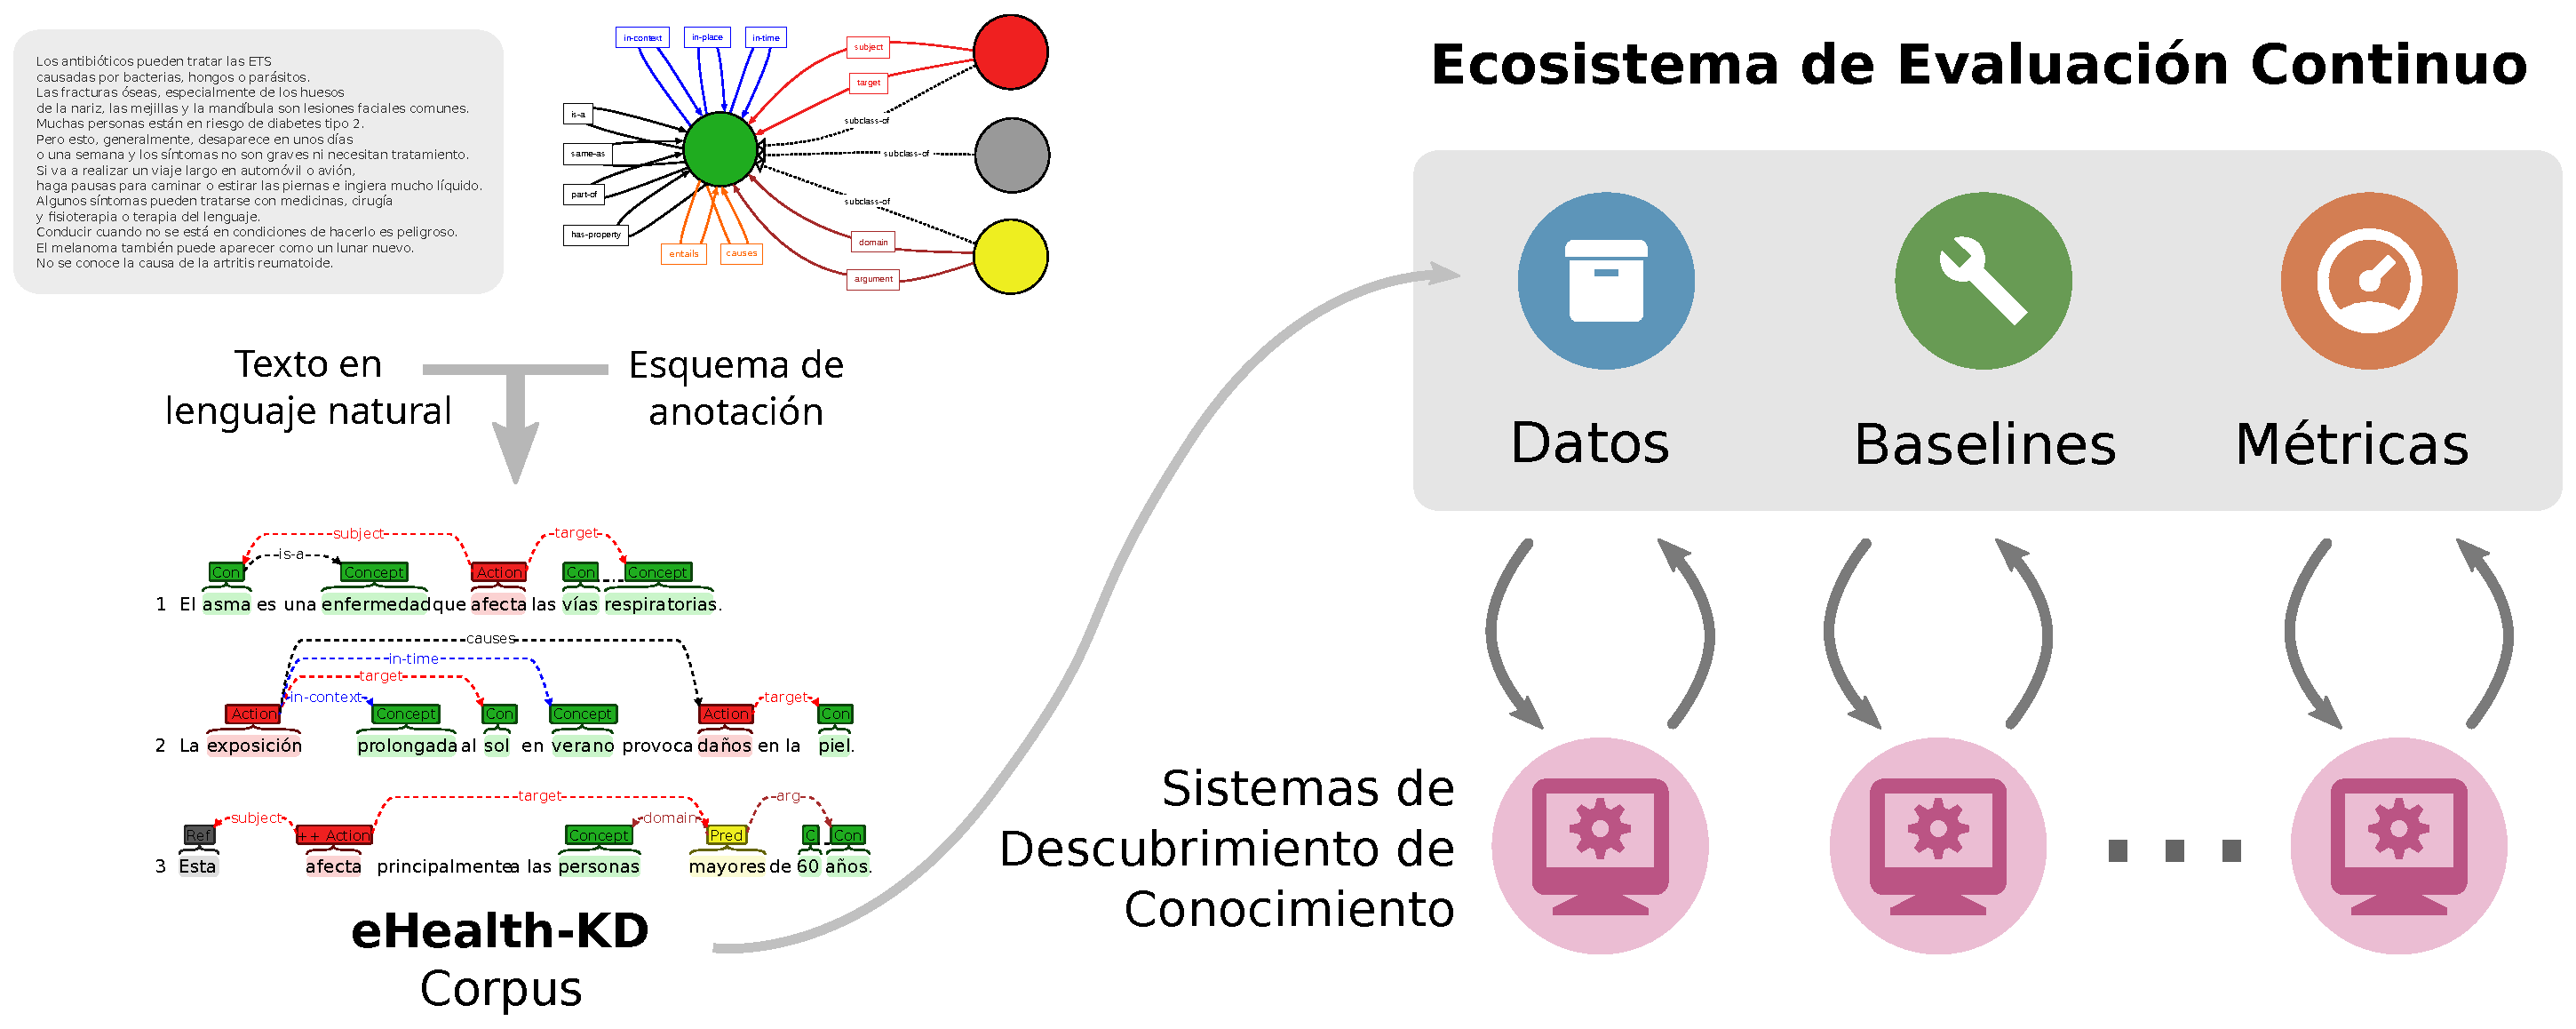
\includegraphics[width=\textwidth]{Images/Chapters/graphical-abstract.pdf}
    \caption{Esquema conceptual del ecosistema computacional diseñado en esta tesis.}
    \label{fig:conceptualmap}
\end{figure}

\section{Esquema de Anotación}\label{results:schema}

El proceso de descubrimiento de conocimiento en lenguaje natural comienza por la identificación en el texto de los conceptos y relaciones más relevantes en un dominio. Para ello es necesario definir un modelo de representación semántico que capture estos conceptos. Dicho modelo se concreta en un esquema de anotación que permite a expertos humanos construir un corpus anotado semánticamente. Construir sistemas de descubrimiento de conocimiento automáticos generalizables a cualquier dominio requiere que los conceptos y relaciones representados sean de propósito general. Además, el esquema de anotación debe lograr un balance adecuado entre su capacidad expresiva y su simplicidad para ser anotado por expertos humanos y algoritmos de aprendizaje automático.

En esta Tesis se propone un esquema de anotación con estas características, que se inspira en varios recursos.
En términos de representación del conocimiento, se basa en dos modelos diferentes para la conceptualización de la realidad: ontologías y teleologías.
La Figura~\ref{fig:example} muestra una anotación de ejemplo de tres oraciones con diferentes grados de complejidad.
El esquema de anotación se explica en profundidad en el Capítulo~\ref{Chap:Schema}.

\begin{figure}[htb]
    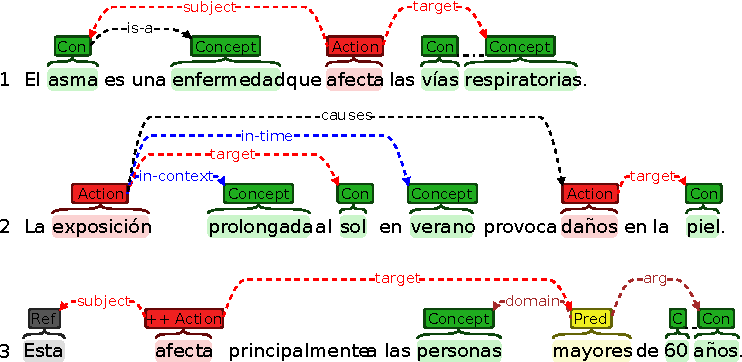
\includegraphics[width=\textwidth]{Images/Chapters/ExampleSentences.pdf}
    \caption[Ejemplos de anotación.]{Ejemplo de anotación de tres oraciones. La anotación muestra las entidades y relaciones más relevantes definidas en el esquema de anotación propuesto.}
    \label{fig:example}
\end{figure}

La parte ontológica del esquema proporciona una representación de entidades en términos de sus relaciones jerárquicas y estructurales~(es decir, \texttt{is-a}, \texttt{part-of}, \texttt{has-property} y \texttt{same-as}).
Estas relaciones se basan en el diseño de ontologías de propósito general como ConceptNet~\cite{speer2017conceptnet} y YAGO~\cite{suchanek2007yago}.
La parte teleológica del esquema proporciona una representación de eventos o procesos que transforman entidades, es decir, representan las interacciones entre las entidades.
Esta parte del esquema está respaldada en una estructura basada en el trabajo de~\citet{teleologies}.
El significado semántico exacto de estos conceptos y relaciones se explica con más detalle a continuación.

El elemento más importante de la anotación es la estructura Sujeto-Acción-Objetivo~(\textit{Subject-Action-Target}), que captura la interacción principal entre entidades en oraciones factuales.
En esta interacción participan dos tipos de entidades fundamentales: \texttt{Concept} y \texttt{Action}.
Un \texttt{Concept} define una entidad relevante en el dominio, que puede ser una sola palabra o múltiples tokens, contiguos o no.
Una \texttt{Action} representa un proceso o evento causado por uno o más \texttt{Concept}~(mediante la relación \texttt{subject}) y que impacta en uno o más \texttt{Concepts}~(mediante la relación \texttt{target}).
Las entidades conectadas a los roles \texttt{subject} y \texttt{target} también pueden ser de tipo \texttt{Action}, lo que permite que los conceptos simples se compongan en otros más complejos.
La estructura Sujeto-Acción-Objetivo definida en este esquema se basa en una versión simplificada del marco teleológico propuesto por~\citet{teleologies}. Los elementos \textit{Object} y \textit{Action} en las teleologías están representados en este esquema por \texttt{Concept} y \texttt {Action} respectivamente.
El rol \textit{Function} en las teleologías, que expresa una instancia de un objeto que realiza una acción, puede equipararse aproximadamente al uso de una entidad de tipo \texttt{Action} ocupando el rol \texttt{subject} o \texttt{target} de otras acciones.

Una adición importante a este esquema de anotación es la entidad \texttt{Predicate}.
Los predicados modelan la existencia de conceptos complejos~(mediante el rol \texttt{domain}) que dependen de algunas condiciones previas~(mediante el rol \texttt{arg}).
Por ejemplo, en la Figura~\ref{fig:example}, Oración 3, el concepto de \textit{personas mayores de 60 años} se puede definir con una anotación detallada, considerando ``\textit{personas}'' como el dominio y ``\textit{60 años}'' como argumento. Esta anotación permite la captura de información más detallada en lugar de simplemente anotar la frase completa como un concepto de varias palabras.
Otra adición es \texttt{Reference}, que representa conceptos mencionados de forma implícita en una oración.
Las palabras más comunes etiquetadas como referencias son: ``\textit{esto}'', ``\textit{el}'', ``\textit{la}'', ``\textit{este}'', es decir , generalmente pronombres y artículos.

Para refinar aún más la interpretación semántica de cada entidad, se define un conjunto de 4 atributos:
\texttt{uncertain}, \texttt{emphasized}, \texttt{diminished} y \texttt{negated}.
Estos atributos a menudo se pueden identificar mediante adjetivos u otros patrones sintácticos que aparecen en el contexto de una entidad determinada, pero en lugar de anotar toda la frase, la entidad correspondiente se etiqueta con el atributo.
Por ejemplo, en la oración 3 de la Figura~\ref{fig:example}, la acción ``\textit{afecta}'' se etiqueta con \texttt{emphasized}, debido a la presencia de la palabra ``\textit{principalmente}'', y se representa en la anotación con un signo \texttt{++} en la entidad.
El uso de atributos permite la captura de conceptos semánticos más refinados~(es decir, grados de énfasis, negación, incertidumbre) mientras se mantiene el agnosticismo del idioma, ya que es irrelevante en qué parte del texto se presenta esa información.
Puede aparecer explícitamente en una sola palabra~(por ejemplo, un adjetivo) o implícitamente mediante frases idiomáticas u otros patrones lingüísticos sutiles.
Estos atributos aumentan el rango semántico del esquema de anotación sin aumentar el número de tokens que deben ser anotados.

Este esquema define 4 relaciones ontológicas principales: \texttt{is-a}, \texttt{same-as}, \texttt{part-of} y \texttt{has-property}, con su semántica habitual, que pueden vincular cualquier par de entidades, simples o compuestas, entre sí.
Estas relaciones permiten la representación del conocimiento estructural, por ejemplo, conceptos relacionados en una estructura jerárquica y conceptos que son componentes de otros conceptos.
Se define dos relaciones adicionales, \texttt{causes} y \texttt{entails}, para capturar causalidad e implicación lógica respectivamente.
Estas relaciones, respectivamente de naturaleza teleológica y ontológica, son de gran importancia porque permiten la construcción de sistemas de razonamiento que pueden llegar a conclusiones y producir nuevos conocimientos a partir de un corpus existente.

Además, se definen 3 relaciones contextuales, para recopilar conocimientos importantes que generalmente aparecen como complementos gramaticales: \texttt{in-time}, \texttt{in-place}, \texttt{in-context}.
La relación \texttt{in-time} se usa para expresar la duración de un evento.
La relación \texttt{in-place} se usa para identificar una ubicación específica para una entidad de tipo \texttt{Action} o \texttt{Concept}.
La relación \texttt{in-context} es una relación más genérica que representa una dependencia general entre dos entidades cuya naturaleza exacta no puede definirse por ninguna de las otras relaciones.
Estas relaciones también son de naturaleza teleológica, ya que no definen una afirmación en sí, sino que son útiles para especificar las condiciones en las que ocurren algunos eventos.
Por ejemplo, en la Oración 2~(Figura~\ref{fig:example}, la anotación \textit{exposición}~$\Rightarrow$~\texttt{in-context}~$\Rightarrow$~\textit {prolongado} no implica que el concepto ``\textit{exposición}'' incondicionalmente tenga la calidad ``\textit{prolongado}''. Solo cuando este concepto complejo se usa como \texttt{subject} o \texttt{target} de una entidad de tipo \texttt{Action} o en otra relación, es que la contextualización adquiere un significado.

La figura~\ref{fig:model} resume el esquema de anotación. Este esquema está diseñado para capturar el conocimiento semántico más relevante presente en un corpus arbitrario.
Por esta razón, no se definieron relaciones o entidades específicas de dominio~(es decir, no hay entidades específicas para enfermedades, pacientes, tratamiento, etc.).
Por el contrario, las relaciones específicas de dominio pueden representarse mediante acciones y sus roles correspondientes.

\begin{figure}[htb]
    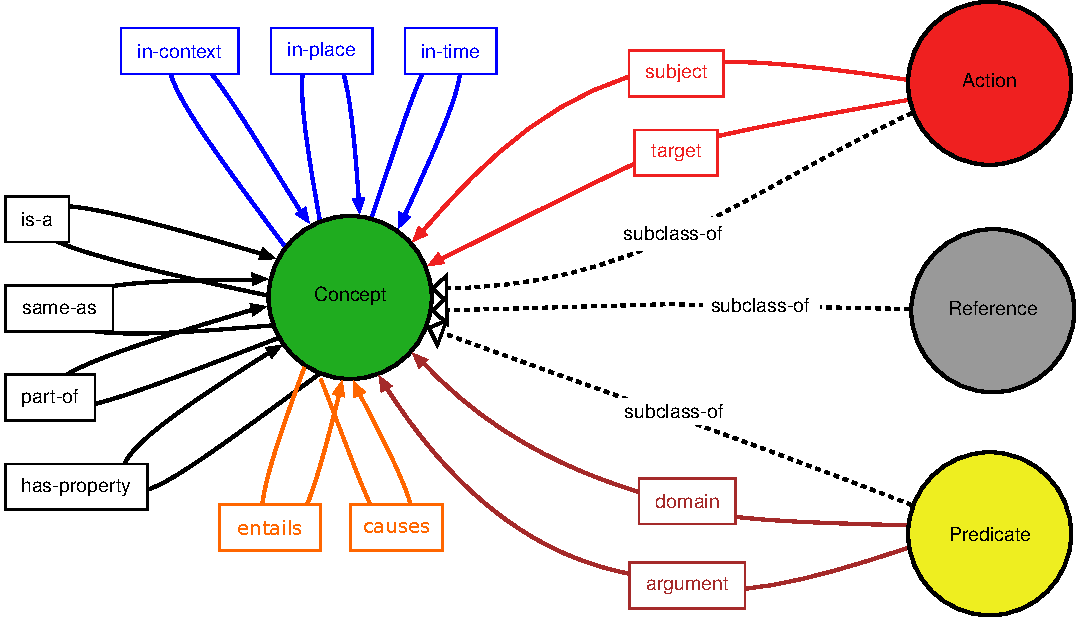
\includegraphics[width=\textwidth]{Images/Chapters/AnnotationModelDiagram.pdf}
    \caption{Diagrama resumen del esquema de anotación general.}
    \label{fig:model}
\end{figure}

\section{Corpus}\label{results:corpus}

Basado en el esquema de anotación definido en la Sección~\ref{results:schema} se anotaron un total de 4 versiones incrementales de un corpus en idioma español.
Cada versión corresponde a una edición de la campaña de anotación \textit{eHealth-KD} que se presenta en la Sección~\ref{results:challenge}. La primera versión se anotó con una variante ligeramente diferente del esquema de anotación, debido a que este esquema fue evolucionando durante el proceso de investigación.
En esta Sección se presentan las características fundamentales de este corpus, incluyendo la estrategia de anotación seguida en cada caso.

\begin{figure}[htb]
    \centering
    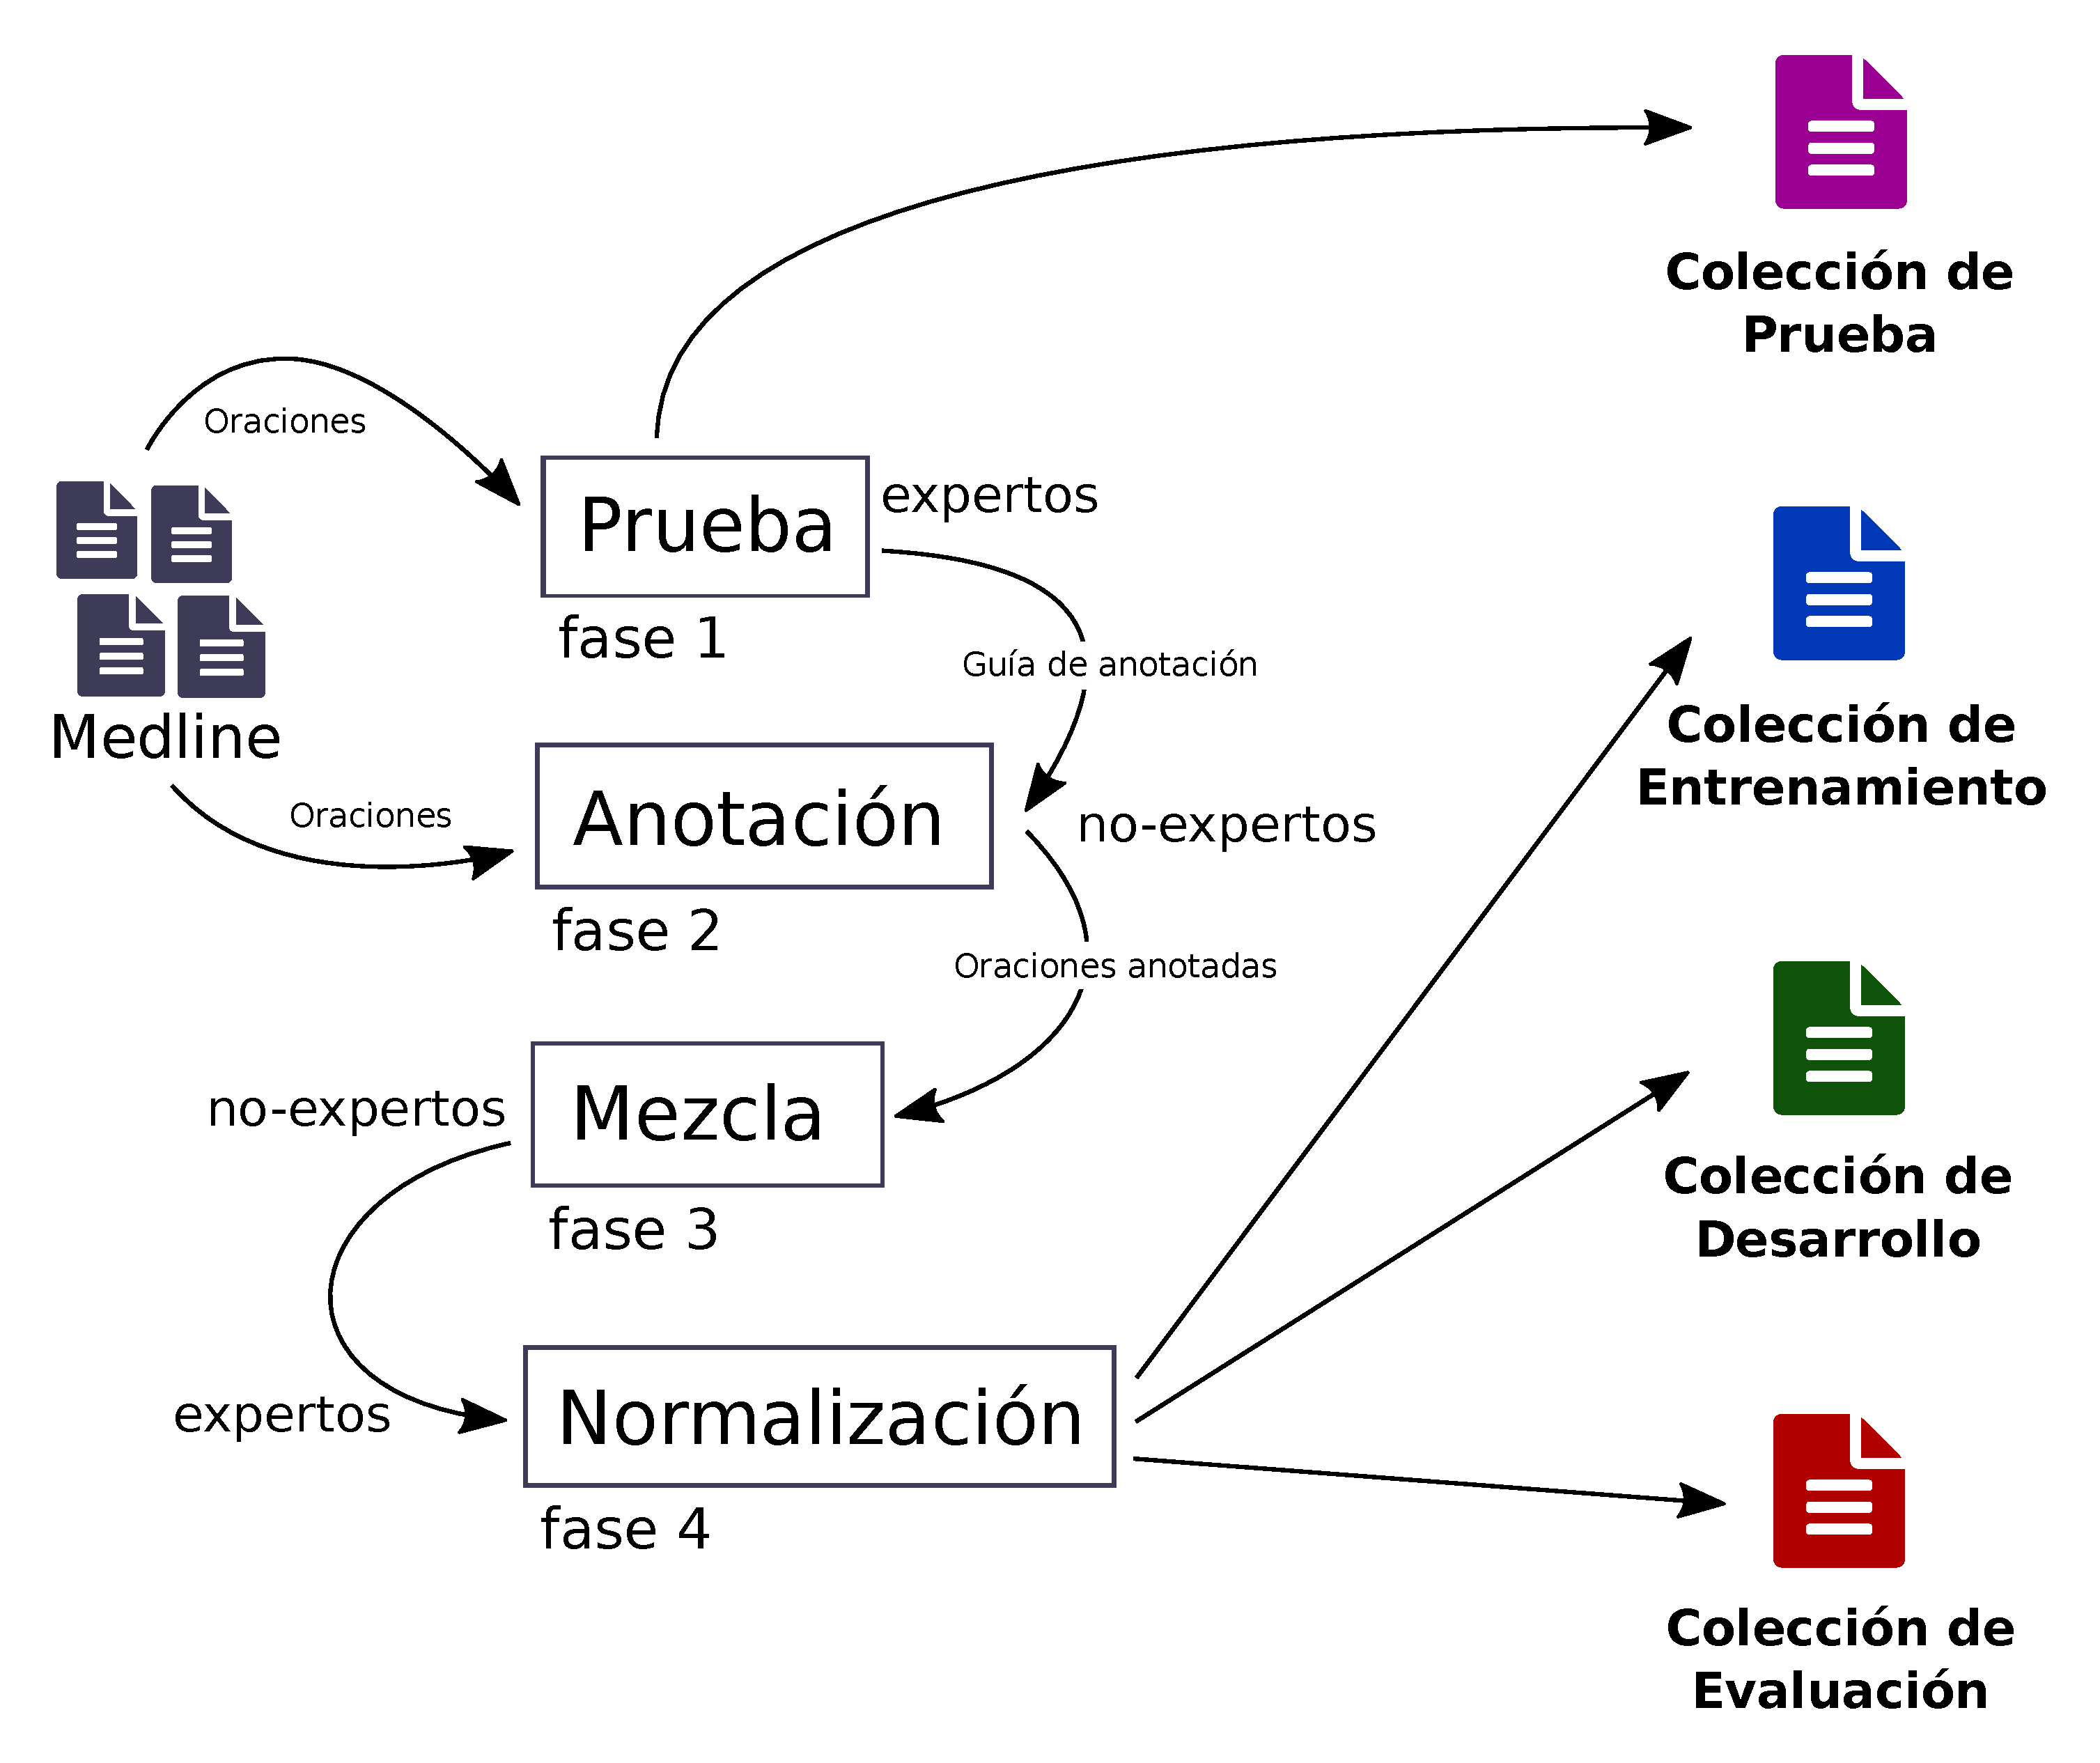
\includegraphics[width=0.9\textwidth]{Images/Chapters/AnnotationProcess.pdf}
    \caption{Esquema general del proceso de anotación.}
    \label{fig:annotation-process}
\end{figure}

La Figura~\ref{fig:annotation-process} describe el proceso de anotación seguido en todos los corpus desarrollados en esta investigación, consistente en 4 etapas fundamentales. En primer lugar un conjunto reducido de anotadores expertos
construye una colección de prueba con un número pequeño de oraciones~(p.e., 50 oraciones), escogidas específicamente
para cubrir la mayor cantidad posible de patrones de anotación. Con esta colección se construye una guía de anotación que se distribuye entre un conjunto de anotadores no-expertos para su entrenamiento y evaluación. Los anotadores no-expertos realizan la anotación manual del resto del corpus, de forma que cada oración es anotada por exactamente dos personas diferentes sin interacción entre sí.
Luego se realiza un proceso de mezcla para escoger entre las 2 versiones anotadas de cada oración.
Para cada oración anotada, esta mezcla la realiza respectivamente uno de los anotadores no-expertos que no haya participado en la primera fase en dicha oración. De esta forma cada oración ha sido evaluada hasta este paso por 3 personas diferentes.
Finalmente, los anotadores expertos revisan en conjunto todas las oraciones anotadas y proponen modificaciones menores que deben ser aprobadas por unanimidad.

Siguiendo este proceso de anotación y el esquema definido en la Sección~\ref{results:schema}, se han construido 4 ediciones del corpus, de tamaño similar, utilizados respectivamente como escenarios de evaluación en las ediciones 2018, 2019, 2020 y 2021 del \textit{eHealth-KD Challenge}.
Aunque la composición exacta del comité de anotadores no-expertos ha variado en cada una de las ediciones, el conjunto de anotadores expertos se ha mantenido constante, y la mayoría de los anotadores no-expertos han participado en más de una edición.
En las cuatro ediciones el grueso de las oraciones se han obtenido de la base de datos \textit{Medline Plus}\footnote{\url{https://medlineplus.gov/xml.html}} que contiene artículos en idioma español (además de inglés) en el dominio de la salud. En la edición 2020 se adicionó como fuente de información un conjunto de $200$ artículos seleccionados aleatoriamente de \textit{Wikinews} para estimular el desarrollo de sistemas de aprendizaje multi-dominio y evaluar cuán generalizable es el esquema de anotación.
En la edición 2021, con motivo de la agravada situación epidemiológica a nivel global propiciada por la pandemia del COVID-19, se adicionaron $200$ oraciones del corpus \texttt{CORD-19}~\cite{wang2020cord} relacionadas con esta enfermedad, en idioma inglés.
De esta forma, la mayoría de las oraciones anotadas son en idioma español, excepto la última colección proveniente de \texttt{CORD-19}.

La Tabla~\ref{tab:corpus} resume las estadísticas fundamentales de los tres corpus anotados, denominados
respectivamente \textit{eHealth-KD} 2018, 2019, 2020 y 2021.
El corpus de la edición 2018~(ver Capítulo~\ref{Chap:CorpusV1}) fue anotado con una versión simplifica del esquema de anotación, dado que aún no se había formalizado completamente. Por este motivo solamente se anotaron acciones, conceptos, y 4 relaciones semánticas. En total se anotaron $1,173$ oraciones que agrupan $13,113$ elementos semánticos.
En la edición 2019~(ver Capítulo~\ref{Chap:CorpusV2}) se introdujeron todos los elementos semánticos del esquema de anotación y se anotaron $1,045$ oraciones nuevas con un total de $13,246$ elementos.
Para la edición 2020 se reutilizaron $1,000$ oraciones de la edición anterior, y se adicionaron $500$ oraciones nuevas siguiendo el mismo esquema de anotación, $300$ de dominio médico y $200$ de artículos periodísticos.
Para la edición 2021 se reutilizaron $1650$ oraciones de la versión anterior, y se anotaron $350$ oraciones nuevas, de ellas $200$ en idioma inglés.
En total se han anotado $3,068$ oraciones en idioma español con $41,163$ elementos semánticos que capturan múltiples patrones lingüísticos en documentos del dominio médico y periodístico, en idiomas español e inglés.

\begin{table}[tpb]
    \centering
    \resizebox{!}{0.425\textheight}{
        \begin{tabular}{lrrrrr}
            \toprule
                                   & \multicolumn{4}{c}{\textbf{Corpus eHealth-KD}}                                                                  \\
                                   & \textbf{2018}                                  & \textbf{2019} & \textbf{2020} & \textbf{2021} & \textbf{Total} \\
            \midrule
            \textit{Oraciones}     & 1,173                                          & 1,045         & ${}^*$1,500   & ${}^*$1,900   & 3,068          \\
            \,\,\,Prueba           & 29                                             & 45            & 0             & 0             & 74             \\
            \,\,\,Entrenamiento    & 559                                            & 600           & ${}^*$800     & ${}^*$1500    & 1,159          \\
            \,\,\,Desarrollo       & 285                                            & 100           & ${}^*$200     & ${}^*$100     & 535            \\
            \,\,\,Evaluación       & 300                                            & 300           & 500           & ${}^*$300     & 1,400          \\
            \midrule
            \textit{Anotaciones}   & 13,113                                         & 13,246        & 8,538         & 6,266         & 41,163         \\
            \midrule
            \textit{Entidades}     & 7,188                                          & 6,612         & 4,237         & 3,162         & 21,199         \\
            \texttt{ Concept}      & 5,366                                          & 4,092         & 2,803         & 2,366         & 14,627         \\
            \texttt{ Action}       & 1,822                                          & 1,742         & 944           & 548           & 5,056          \\
            \texttt{ Predicate}    & -                                              & 563           & 420           & 225           & 1,208          \\
            \texttt{ Reference}    & -                                              & 215           & 70            & 23            & 308            \\
            \midrule
            \textit{Relaciones}    & 5,925                                          & 6,049         & 4,037         & 2,934         & 18,945         \\
            \texttt{ target}       & 2,120                                          & 1,729         & 855           & 483           & 5,187          \\
            \texttt{ subject}      & 1,466                                          & 894           & 706           & 340           & 3,406          \\
            \texttt{ is-a}         & 1,057                                          & 566           & 383           & 241           & 2,247          \\
            \texttt{ part-of}      & 393                                            & 94            & 57            & 28            & 572            \\
            \texttt{ has-property} & 836                                            & 159           & 111           & 272           & 1,378          \\
            \texttt{ same-as}      & 53                                             & 124           & 85            & 43            & 305            \\
            \texttt{ in-context}   & -                                              & 677           & 584           & 674           & 1,935          \\
            \texttt{ in-place}     & -                                              & 400           & 351           & 285           & 1,036          \\
            \texttt{ in-time}      & -                                              & 165           & 215           & 120           & 500            \\
            \texttt{ domain}       & -                                              & 364           & 285           & 141           & 790            \\
            \texttt{ argument}     & -                                              & 343           & 233           & 111           & 687            \\
            \texttt{ causes}       & -                                              & 367           & 131           & 103           & 601            \\
            \texttt{ entails}      & -                                              & 167           & 41            & 72            & 280            \\
            \midrule
            \textit{Attributos}    & -                                              & 585           & 264           & 170           & 1,019          \\
            \texttt{ diminished}   & -                                              & 18            & 11            & 13            & 42             \\
            \texttt{ emphasized}   & -                                              & 124           & 80            & 59            & 263            \\
            \texttt{ negated}      & -                                              & 164           & 72            & 41            & 277            \\
            \texttt{ uncertain}    & -                                              & 279           & 101           & 57            & 437            \\
            \bottomrule
        \end{tabular}}
    \caption[Estadísticas del corpus \textit{eHealth-KD}.]{Estadísticas de las 4 ediciones del corpus \textit{eHealth-KD}. Los números anotados con ${}^*$ en 2020 y 2021 indican que se han reutilizado oraciones de las ediciones anteriores. En este caso solo se contabilizan en el total las anotaciones las oraciones nuevas anotadas en cada edición.}
    \label{tab:corpus}
\end{table}

\section{Definición de Tareas}\label{results:tasks}

Los recursos lingüísticos presentados en la Sección~\ref{results:corpus} son necesarios para entrenar sistemas computacionales que sean capaces de extraer automáticamente contenido semántico de lenguaje natural. Para avanzar en esta tarea es conveniente diseñar un entorno de evaluación que permita comparar de forma objetiva los enfoques posibles. Para evaluar mejor las fortalezas y debilidades de los diferentes enfoques, la tarea de anotación automática se divide en dos subtareas:

\begin{description}
    \item[Subtarea A: Reconocimiento de Entidades.]
          El propósito de esta subtarea es identificar todas las entidades mencionadas en una oración y sus clases correspondientes.~(i.e., \texttt{Concept}, \texttt{Action}, \texttt{Predicate} y \texttt{Reference}.

    \item[Subtarea B: Extracción de relaciones.]
          El propósito de esta subtarea es detectar todas las relaciones semánticas entre cada par de entidades ya etiquetadas en cada oración.
\end{description}

Como criterio de evaluación de ambas subtareas se propone una versión extendida de la métrica $F_1$ modificada para tratar coincidencias parciales. La métrica $F_1$ depende de las anotaciones correctas, incorrectas, parciales, faltantes y espurias en todo el conjunto de evaluación. Dependiendo de la(s) subtarea(s) bajo evaluación, definimos los siguientes tipos de resultados:

\begin{description}
    \item[Subtarea A - Correctos $C_A$:] cuando una anotación coincide exactamente con la anotación correcta correspondiente.
    \item[Subtarea A - Incorrectos $I_A$:] cuando una anotación coincide con una anotación correcta con respecto al espacio de texto pero define una etiqueta de entidad diferente.
    \item[Subtarea A - Parciales $P_A$:] cuando un fragmento de texto tiene una intersección no vacía pero inexacta con una anotación correcta, como el caso de ``\textit{vías respiratorias}'' y ``\textit{vías}'' en la Figura~\ref{fig:example}, oración 2.
          Las frases parciales solo se comparan con una frase correcta~(es decir, la primera frase parcialmente coincidente desde el principio de la oración) para evitar que algunos fragmentos de texto grandes que cubren la mayor parte del documento obtengan una puntuación muy alta.
    \item [Subtarea A - Faltantes $M_A$:] cuando no se produce una anotación que aparece en la colección de anotaciones correctas.
    \item [Subtarea A - Espurios $S_A$:] cuando se produce una anotación que no aparece en la colección de anotaciones correctas.
\end{description}

\begin{description}
    \item[Subtarea B - Correctos $C_B$:] cuando existe una relación entre dos entidades en la colección de anotaciones correctas.
    \item[Subtarea B - Faltantes $M_B$:] cuando no se produce una relación en la colección de anotaciones correctas.
    \item[Subtarea B - Espurios $S_B$:] cuando se produce una relación pero no aparece en la colección de anotaciones correctas.
\end{description}

Se define $Precision$, $Recall$, y $F_1$ de la manera usual, teniendo en cuenta que para cada escenario de evaluación solo se consideran los términos relacionados con la(s) subtarea(s) bajo evaluación.

\begin{eqnarray}
    Precision & = & \frac{C_A + C_B + \frac{1}{2} P_A}{C_A + I_A + C_B + P_A + S_A + S_B} \\
    Recall    & = & \frac{C_A + C_B + \frac{1}{2} P_A}{C_A + I_A + C_B + P_A + M_A + M_B} \\
    F_1       & = & 2 \cdot \frac{Precision \cdot Recall}{Precision + Recall} \label{eqn:f1}
\end{eqnarray}{}

Finalmente, se propone $F_1$ como se define en la Ecuación~\ref{eqn:f1} como la métrica oficial para comparar diferentes enfoques. En cada versión del corpus \textit{eHealth-KD} se define un subconjunto diferente de oraciones para evaluar cada subtarea de forma independiente o ambas tareas de manera simultánea.

\section{Infraestructura de Aprendizaje y Evaluación}\label{results:infrastructure}

Para apoyar a los investigadores en el desarrollo de tecnologías de descubrimiento de conocimiento, se proporciona un conjunto de herramientas e infraestructura que permiten un proceso de experimentación más rápido y objetivo.
Estos recursos están disponibles gratuitamente para la comunidad científica en una colección de repositorios de Github\footnote{\url{https://ehealthkd.github.io}}.
El conjunto de recursos desarrollado consiste en los siguientes elementos:

\begin{itemize}
    \item Archivos de texto plano y anotaciones en formato BRAT Standoff~\cite{brat} para el corpus \textit{eHealth-KD}, dividido en colecciones de entrenamiento, desarrollo y evaluación.
    \item Archivos de configuración necesarios para desplegar un servidor BRAT con el objetivo de analizar y ampliar el corpus \textit{eHealth-KD}, o para crear otros recursos lingüísticos basados en el esquema de anotación descrito en la Sección~\ref{results:schema}.
    \item Herramientas en el lenguaje de programación Python para cargar y manipular las anotaciones de BRAT Standoff así como para producir resultados formateados correctamente.
    \item Herramientas para configurar y ejecutar algoritmos de evaluación para la tarea definida en la Sección~\ref{results:tasks}, incluidas las subtareas, y calcular las métricas de evaluación oficiales.
    \item Un conjunto de implementaciones de algoritmos de aprendizaje básicos con diferentes grados de complejidad, incluida una estrategia aleatoria y varios enfoques clásicos.
\end{itemize}

Usando las herramientas antes mencionadas, los investigadores pueden desarrollar rápidamente nuevos enfoques extendiendo las implementaciones \textit{baseline} o desarrollando una solución desde cero, sin tener que lidiar con la configuración del entorno o la implementación de las métricas de evaluación.
Además de poder evaluar sus soluciones personalmente, los investigadores también pueden subir sus soluciones a un entorno de evaluación en la nube y obtener automáticamente las métricas relevantes así como comparar sus resultados con soluciones ya publicadas.
Se mantiene una tabla de clasificación oficial que sirve como un estado del arte actualizado en todas las subtareas.

\section{Evaluación de Sistemas}\label{results:challenge}

Las cuatro versiones del corpus \textit{eHealth-KD} presentadas en la Sección~\ref{results:corpus} han sido utilizadas en la evaluación de sistemas de extracción de conocimiento diseñados por diversos equipos de investigadores en el marco del evento \textit{eHealth Knowledge Discovery}, organizado en los años 2018, 2019, 2020 y 2021.
En la Tabla~\ref{tab:results-challenge} se resumen los resultados más importantes de las cuatro ediciones de este evento.
Se reportan el número de participantes (equipos de investigadores), los mejores resultados alcanzados tanto en el proceso completo de extracción como en cada una de las subtareas definidas en la Sección~\ref{results:tasks}~(en términos de la métrica $F_1$), así como un resumen de las técnicas más utilizadas.

\begin{table}[htb]\centering
    \begin{tabular}{lrrrr}
        \toprule
                                     & \bf 2018 & \bf 2019 & \bf 2020 & \bf 2021 \\
        \midrule
        Equipos Registrados          & 31       & 30       & 26       & 30       \\
        Equipos Participantes        & 6        & 10       & 8        & 9        \\
        \midrule
        Resultados generales         & 0.744    & 0.639    & 0.660    & 0.531    \\
        Subtarea A (entidades)       & 0.872    & 0.820    & 0.825    & 0.706    \\
        Subtarea B (relaciones)      & 0.448    & 0.626    & 0.633    & 0.430    \\
        \midrule
        \textbf{Técnicas}            &          &          &          &          \\
        PLN clásico                  & 5        & 7        & 0        & 3        \\
        Reglas                       & 2        & 2        & 3        & 1        \\
        \textit{Embeddings}          & 2        & 7        & 8        & 9        \\
        Redes neuronales             & 3        & 10       & 7        & 9        \\
        \textit{Transformers}        & 0        & 1        & 5        & 8        \\
        Conocimiento externo         & 2        & 1        & 3        & 9        \\
        Solución \textit{end-to-end} & 0        & 1        & 2        & 3        \\
        \bottomrule
    \end{tabular}
    \caption[Resultados del \textit{eHealth Knowledge Discovery}]{Resumen de los resultados de las tres ediciones del \textit{eHealth Knowledge Discovery} y las técnicas más comúnmente aplicadas en cada edición.\label{tab:results-challenge}
    }\end{table}

Con respecto a los resultados obtenidos en la solución de las tareas, es necesario reconocer que la complejidad de la edición 2018 es significativamente menor debido a que existe un menor número de tipos de entidades y relaciones.
Por este motivo los resultados no son directamente comparables con los de las ediciones 2019, 2020 y 2021.
De la misma forma, la edición 2021 incluyó tres dominios y dos idiomas, por lo que es de esperar que los resultados sean ligeramente inferiores a las ediciones anteriores.
Aún así, una posible conclusión de estos resultados es que la detección de entidades está de manera general resuelta mientras que la extracción de relaciones consiste en el mayor reto.

Analizando las técnicas más utilizadas por los sistemas presentados en cada edición, se puede notar una tendencia hacia los sistemas \textit{end-to-end} basados en arquitecturas de redes neuronales, o sea, sistemas que resuelven ambas tareas como parte de una misma arquitectura en vez de como pasos separados.
De manera general las redes neuronales, y en particular los \textit{embeddings}~(e.g., word2vec, glove) y las arquitecturas \textit{transformer}~(e.g., BERT, GPT), han reemplazado a las técnicas clásicas de procesamiento de lenguaje natural.
Sin embargo, aún es necesario el uso de ciertas reglas específicas del dominio, por ejemplo, para resolver el problema de las entidades superpuestas.
Por otro lado, los enfoques que aprovechan conocimiento externo, aunque no son mayoría siguen teniendo importancia, fundamentalmente en la forma de \textit{embeddings} de dominio específico.

\section{Anotación Asistida}\label{results:assisted-ann}

El proceso de anotación, mezcla y normalización que se ha llevado a cabo durante el transcurso de esta investigación ha permitido reconocer la importancia de esta fase como parte del desarrollo de sistemas de aprendizaje automático y descubrimiento de conocimiento.
La construcción de recursos lingüísticos anotados por expertos es fundamental para entrenar este tipo de sistemas, y consiste en una de las tareas más costosas en términos de esfuerzo humano.
Además, si no se cuenta con una planificación ideal, es probable que los recursos creados sean menos efectivos. Por ejemplo, pueden contener oraciones repetidas o semánticamente similares, conjuntos desbalanceados de etiquetas, y contradicciones internas.
Una forma de aliviar estos problemas y acelerar el proceso de anotación es introducir un mecanismo de aprendizaje automático dentro del propio ciclo de anotación, mezcla y normalización, que ayude a seleccionar los mejores ejemplos a anotar y garantice que no existe redundancia innecesaria en el corpus.

Como parte de esta investigación se propone una estrategia de aprendizaje activo diseñada para un corpus arbitrario de oraciones en lenguaje natural, cada una de las cuales debe ser anotada por un experto humano a nivel semántico, tal y como ocurre con el esquema de anotación propuesto en la Sección~\ref{results:schema}.
Con el objetivo de diseñar una propuesta generalizable, se considera un conjunto arbitrario $\mathcal{E}$ de etiquetas de entidades, cada una de las cuales puede abarcar uno o más tokens, continuos o discontinuos,
y un conjunto predefinido $\mathcal{R}$ de tipos de relaciones binarias entre entidades.
Este modelo de anotación abstracto puede representar una amplia gama de tareas diferentes, incluyendo el corpus \textit{eHealth-KD} en el cuál se inspira, pero abarcando además desde la extracción de relaciones de  dominio específico (por ejemplo, interacción gen-proteína) hasta la representación semántica de propósito general (por ejemplo, análisis de AMR).
Esta estrategia se describe en detalle en el Capítulo~\ref{Chap:Annotation}.

\begin{figure}[htb]
    \centering
    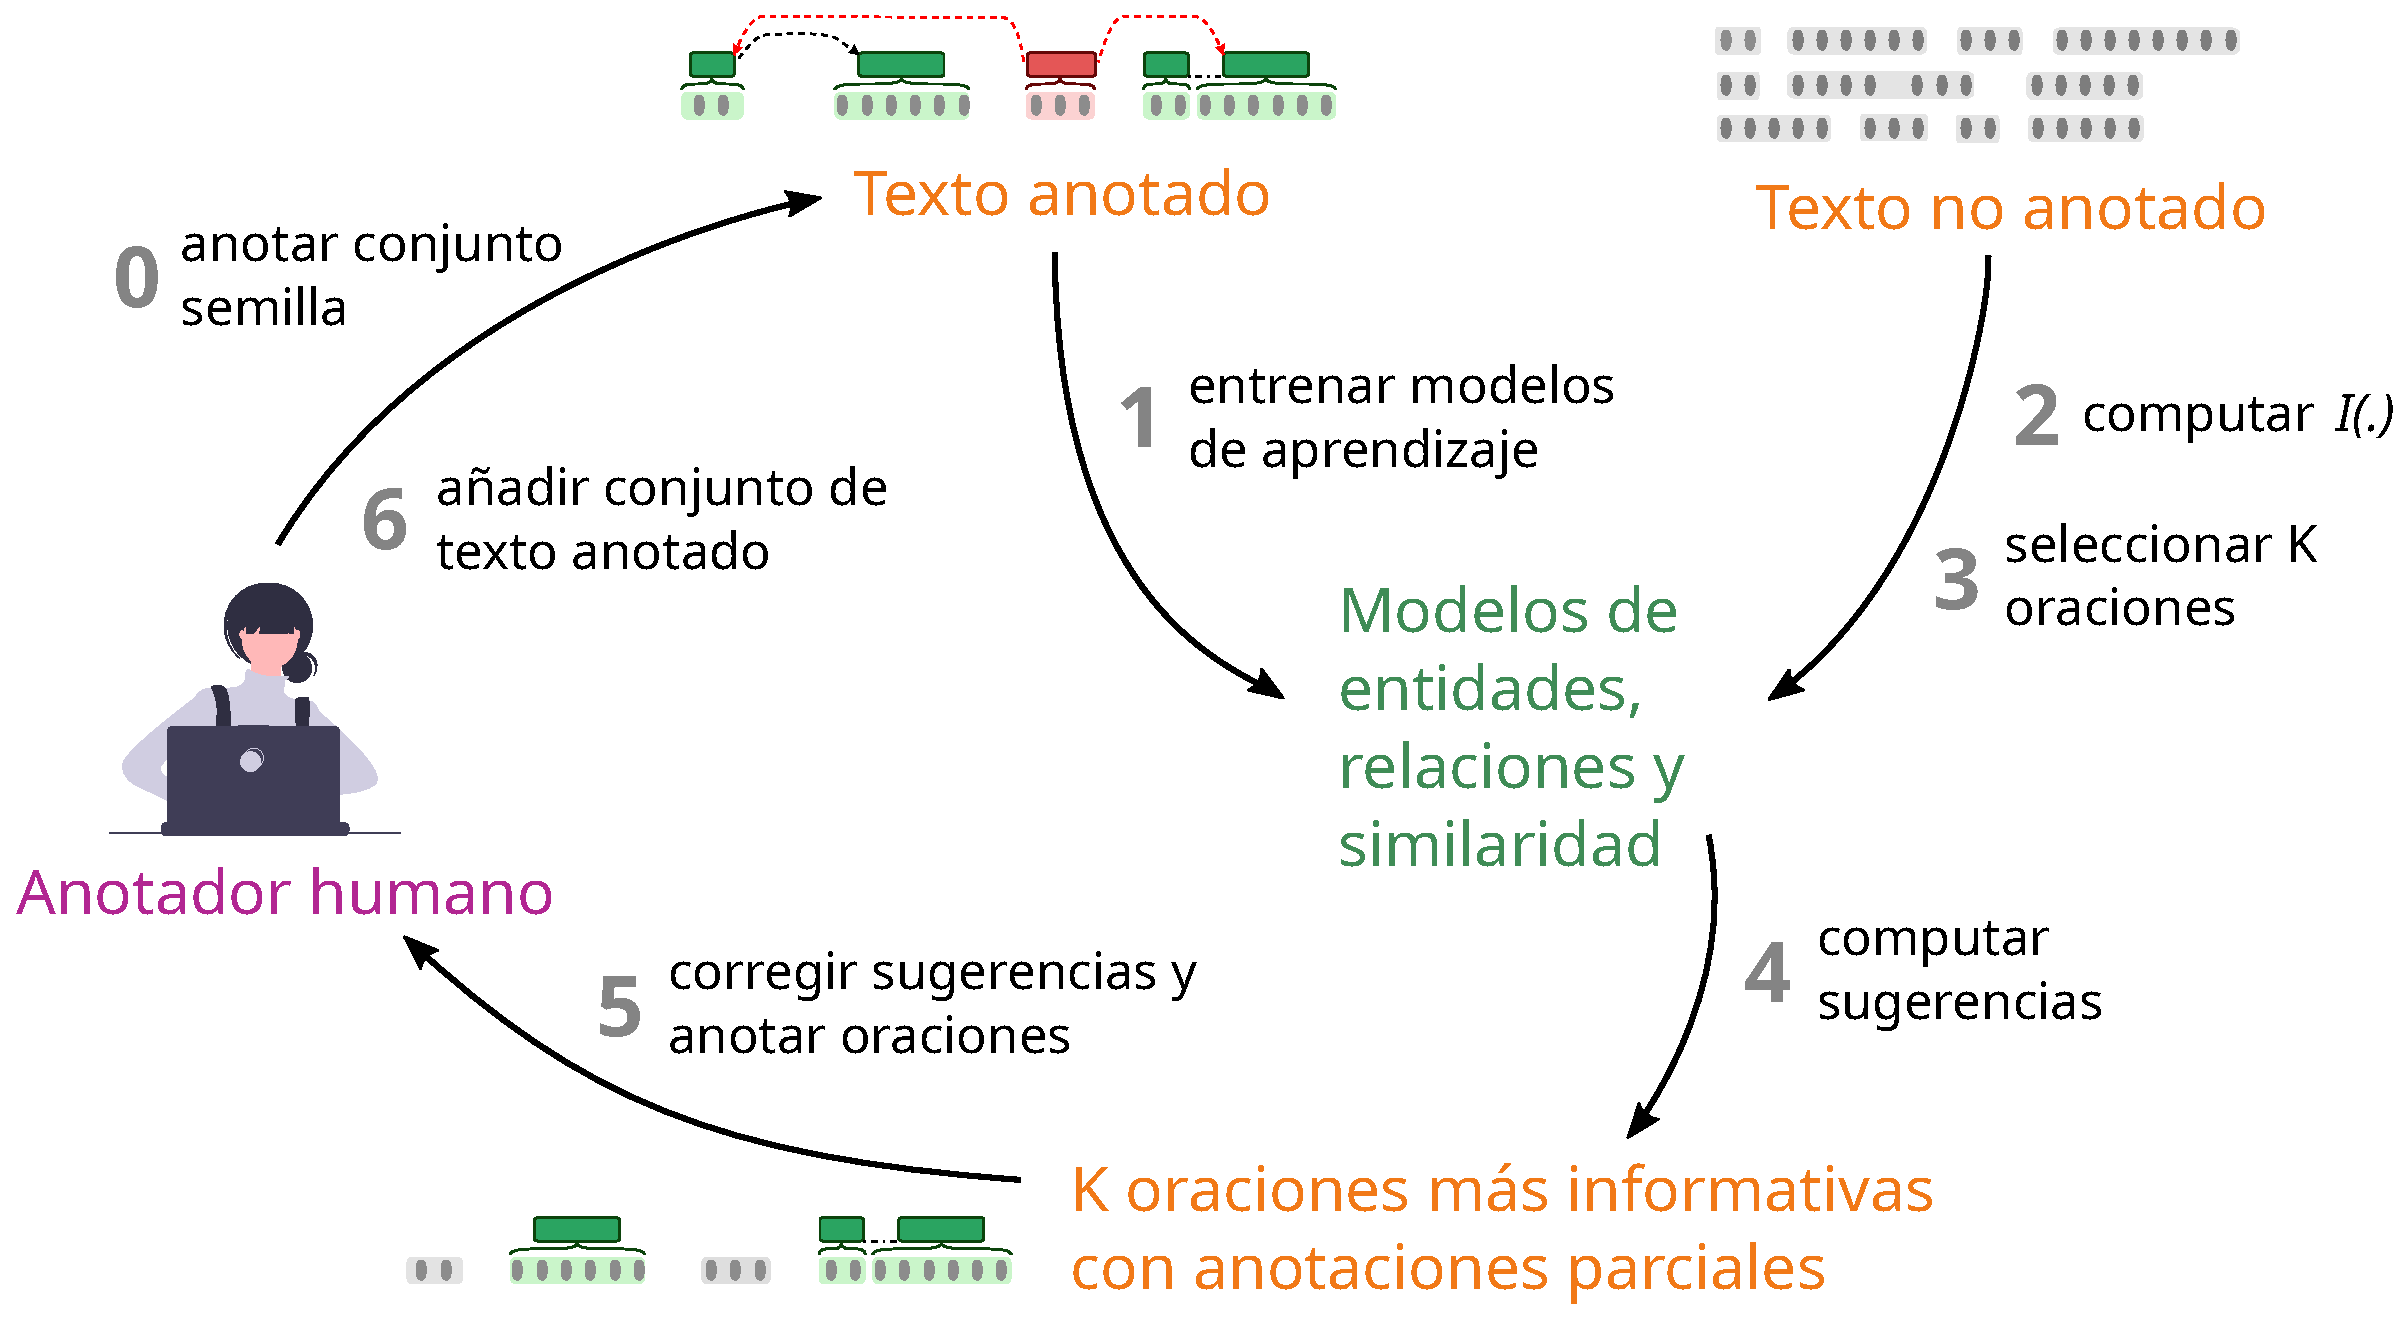
\includegraphics[width=\textwidth]{Images/Chapters/SchemaAssistedAnnotation.pdf}
    \caption[Estrategia de aprendizaje activo.]{Ilustración de alto nivel de la estrategia de aprendizaje activo presentada en esta investigación para la anotación asistida del corpus ehealth-KD.}
    \label{fig:assisted-annotation}
\end{figure}

\newcommand{\Labeled}{\mathbf{L}}
\newcommand{\Unlabeled}{\mathbf{U}}
\newcommand{\infr}[1]{I(#1)}
\newcommand{\infrc}{\infr{\cdot}}
\newcommand{\unc}[1]{H(#1)}
\newcommand{\uncc}{\unc{\cdot}}
\newcommand{\id}[1]{ID(#1)}
\newcommand{\uncm}[1]{\hat{H}(#1)}
\newcommand{\unccm}{\uncm{\cdot}}

La estrategia de aprendizaje activo propuesta en esta investigación funciona de forma iterativa en lotes de $K$ oraciones~(por ejemplo, $K=10$).
La figura~\ref{fig:assisted-annotation} muestra un resumen del proceso.
En cada iteración, existe un conjunto etiquetado $\Labeled$ con $|\Labeled|=n \times K$ oraciones anotadas manualmente por un anotador humano, y un conjunto mayor  $\Unlabeled$ de oraciones no etiquetadas.
Inicialmente, el anotador humano selecciona $K$ oraciones representativas y realiza una anotación manual completa~(paso 0).
Posteriormente, dos modelos de aprendizaje automático se entrenan iterativamente en las oraciones etiquetadas manualmente~(paso 1) y una métrica de \textit{informatividad}, $\infr{s}$, se calcula para cada oración $s \in \Unlabeled$~(paso 2).
Las mejores oraciones $K$ en términos de $\infrc$ se seleccionan~(paso 3) y el modelo produce una predicción de entidades y relaciones para cada una~(paso 4).
Cada predicción tiene una métrica de \textit{incertidumbre} asociada, $\uncc$, estimada por los modelos.
En función de esta incertidumbre y umbrales predefinidos $u_e$ y $u_r$ para entidades y relaciones respectivamente, todas las entidades $e_i$ (relaciones $r_j$) con una incertidumbre estimada $\unc{e_i}>u_e$ ($\unc{r_j}>u_r$) se descartan.
Finalmente, las oraciones seleccionadas y parcialmente anotadas se presentan al anotador humano, quien debe corregir las anotaciones incorrectas y agregar las anotaciones faltantes~(paso 5).
Las oraciones corregidas se incorporan al grupo etiquetado para la siguiente iteración~(paso 6).

Para estimar la informatividad $\infr{s_i}$ de cada oración $s_i \in \Unlabeled$, se define una métrica basada en el modelo de \textit{uncertainty sampling}~\cite{settles2008analysis}.
Dado un conjunto de $n$ anotaciones de entidades $E_i \subseteq \mathcal{E}^n = \{ e^i_1, \ldots, e^i_n \}$ y $m$ anotaciones de relaciones $R_i \subseteq \mathcal{R}^m = \{ r^i_1, \ldots, r^i_m \}$ producidas para una oración $s_i$, se define la incertidumbre de cada entidad $e^i_k$ (o relación $r^i_k$) como la entropía de la distribución de probabilidades de cada una de las posibles etiquetas para dicha entidad o relación. Formalmente:

\small
$$
    \unc{e^i_k} = -\sum_{l_j \in \mathcal{E}} P(e^i_k=l_j | s_i;\theta) \log_2 P(e^i_k=l_j | s_i;\theta)
$$
$$
    \unc{r^i_k} = -\sum_{l_j \in \mathcal{R}} P(r^i_k=l_j | s_i;\theta) \log_2 P(r^i_k=l_j | s_i;\theta)
$$
\normalsize

\noindent
Donde $\theta$ representa los parámetros del modelo de aprendizaje que se utiliza para estimar estas probabilidades.

De la misma forma se puede definir la incertidumbre media asociada a las entidades y relaciones producidas, respectivamente:

\small
$$
    \uncm{E_i} = \frac{1}{n} \sum_{e^i_k \in E_i} \unc{e^i_k} \,\,\,\,\,\,\,\, \uncm{R_i} = \frac{1}{m} \sum_{r^i_k \in R_i} \unc{r^i_k}
$$
\normalsize

Además, se define una métrica de densidad de información $\id{s_i}$ para estimar cuán representativa es cada oración $s_i$
con respecto al conjunto de oraciones anotadas. De forma similar a~\citet{settles2008analysis},
$\id{s_i}$ se define como la similaridad promedio de la oración $s_i$ a un conjunto $K$ de oraciones anotadas:

\small
$$
    \id{s_i} = \frac{1}{K} \sum_{s_j \in \Labeled_i^*} sim(s_i, s_j)
$$
\normalsize

\noindent Donde $\Labeled_i^*$ es el subconjunto de las $K$ oraciones anotadas que maximizan la similaridad con respecto a $s_i$. Cualquier métrica de similaridad podría ser utilizada, pero en esta investigación se propone usar \textit{embeddings} de \textit{Doc2Vec}~\cite{doc2vectgensim}
pre-entrenados en el conjunto $\Unlabeled$ de oraciones no anotadas.

Finalmente, la \textit{informatividad} total de una oración no anotada $s_i$ se estima a partir de la incertidumbre de cada componente (entidad o relación) ponderados por la densidad de información de la oración:

\small
$$
    \infr{s_i} = \left[ \uncm{E_i} + \uncm{R_i} \right] \times \id{s_i}^{\beta}
$$
\normalsize

Para evaluar la efectividad de este enfoque se simula el proceso de anotación asistida en el corpus \textit{eHealth-KD} 2019, comparando las estrategias de aprendizaje activo con la anotación en el orden original sin sugerencias~(como modelo de base).
Como el proceso de anotar un corpus es costoso, la simulación se basa en las anotaciones correctas de la colección de entrenamiento.
La mejora se puede estimar comparando cuántas oraciones necesitan anotaciones para alcanzar un rendimiento específico de los algoritmos de aprendizaje automático~(medido en términos de $F_1$ en la colección de pruebas).

Para ilustrar el grado de reducción de tiempo alcanzado, la Figura~\ref{fig:graph2} muestra el número mínimo de oraciones que deben anotarse para alcanzar diferentes puntajes relativos de $F_1$.
Por ejemplo, después de anotar las primeras $400$ oraciones, es posible lograr un $95\%$ del resultado final de $F_1$ cuando se utiliza todo el corpus.
Sin embargo, para alcanzar la puntuación objetivo, las primeras $880$ oraciones de las $1000$ totales deben anotarse si el corpus se anota en el orden original~(seguido por el modelo de base).
Por el contrario, la estrategia de aprendizaje activo solo requiere anotar entre $530$ y $580$ oraciones para alcanzar el mismo valor de $F_1$, ahorrando así entre $35\%$ y $40\% $ del tiempo de anotación humano.

\begin{figure}[tb]
    \centering
    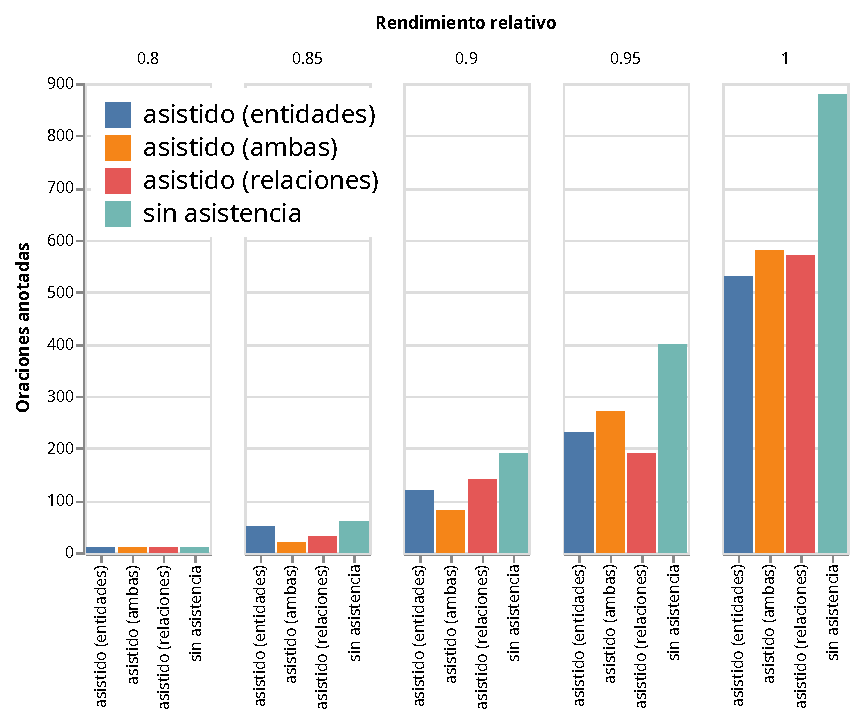
\includegraphics[width=0.8\columnwidth]{Images/Chapters/CostReductionAssistedAnnotation.pdf}
    \caption[Evaluación de la estrategia de aprendizaje activo]{Número mínimo de oraciones necesarias para alcanzar un rendimiento específico en relación con la métrica $F_1$ con cada estrategia de aprendizaje activa para la sugerencia de oraciones.}
    \label{fig:graph2}
\end{figure}

Otro análisis interesante es estimar hasta qué punto las anotaciones sugeridas reducen aún más el tiempo total de anotación.
Un anotador humano que use esta herramienta deberá aceptar algunas de las anotaciones sugeridas, corregir las incorrectas y anotar las faltantes.
Cada una de estas acciones tiene un costo diferente.
Para cuantificar la mejora en el tiempo general que producen las sugerencias, se asigna un costo relativo~(en términos de unidades de tiempo abstractas) a cada uno de los siguientes tipos de anotaciones:

\begin{description}
    \item [Faltantes:] 1 unidad de tiempo.
    \item [Espurias:] 2 unidades de tiempo.
    \item [Correctas:] 0.25 unidades de tiempo.
    \item [Parciales:] 0.5 unidades de tiempo.
\end{description}

Esta estructura de costos asume que el problema de corregir anotaciones incorrectas es más complejo que simplemente producir las anotaciones correctas, al tiempo que reconoce que incluso estar de acuerdo con las anotaciones correctas tiene un costo.
Para que una estrategia de aprendizaje activo sea útil, debe proporcionar suficientes anotaciones correctas para superar el costo de corregir las anotaciones incorrectas; por lo tanto, debe priorizar la precisión sobre el recobrado.
Una simulación de este proceso para diferentes valores de los umbrales de incertidumbre arroja que, en el caso óptimo, se reduce a un $76\%$ el costo de arreglar una oración parcialmente anotada con respecto a la anotación manual.

Se puede estimar una reducción general en el tiempo de anotación para esta simulación experimental combinando las mejoras proporcionadas por las sugerencias de anotación y el orden de las oraciones.
Asumiendo que ambos efectos son independientes, el mejor de los casos para este corpus sugiere lo siguiente.
Usando el enfoque de aprendizaje activo, un anotador humano habría necesitado anotar solo $530$ oraciones de $ 1000$, cada una de ellas con un costo de tiempo estimado de $76\%$ en comparación con la anotación completa.
Esto da como resultado una reducción general de hasta $60\%$ del tiempo de anotación total, produciendo un corpus más pequeño en el que los modelos de aprendizaje automático aún pueden ser entrenados, ofreciendo el mismo rendimiento que los modelos entrenados en el corpus original.

\section{Discusión}
\label{chap2:discussion}

Esta sección presenta una discusión general de las principales contribuciones de esta investigación, las lecciones aprendidas y las limitaciones de las soluciones actuales propuestas para la tarea \textit{eHealth Knowledge Discovery}.
También se destacan ideas interesantes para la investigación futura, basadas en los conocimientos obtenidos al analizar los enfoques más prometedores.

\subsection{Contribuciones}

Se han desarrollado diferentes representaciones semánticas para capturar el conocimiento expresado en lenguaje natural~(p.e., \texttt{AMR}, \texttt{FrameNet} y \texttt{PropBank}, ver Sección~\ref{sec:sota-annotation}).
El principal inconveniente de estas representaciones es su complejidad, ya que a menudo dependen de lexicones que definen los roles semánticos específicos para cada palabra.
Por lo tanto, desarrollar sistemas de inteligencia artificial para el descubrimiento del conocimiento con este nivel de detalle es aún un problema no resuelto.
El uso de representaciones semánticas más simples, que no se basen en roles o relaciones específicas, puede simplificar el desarrollo de técnicas basadas en el aprendizaje automático.

Esta investigación propone una línea de desarrollo en esta dirección, donde el descubrimiento de conocimiento con un alto nivel de abstracción pueda ser refinado posteriormente para tareas de dominio específico.
El propósito no es reemplazar las representaciones semánticas detalladas, como \texttt{AMR} o \texttt{FrameNet}, sino proporcionar una representación más general que se pueda usar como un paso inicial en diferentes tareas de descubrimiento de conocimiento.
Este tipo de representación semántica puede simplificar tareas posteriores como el aprendizaje de ontologías, de la misma manera que el etiquetado POS-tag de propósito general a menudo se realiza antes de tareas de PLN más complejas.
Basado en las experiencias obtenidas durante el proceso de anotación, mezcla y normalización, se ha diseñado un mecanismo para la anotación semi-automática.
En los experimentos realizados se pudo comprobar cómo utilizando modelos de aprendizaje relativamente sencillos se puede acelerar considerable el proceso de anotación.

Los recursos, herramientas e infraestructura desarrollados en esta investigación tienen como objetivo proporcionar una base para que la comunidad científica construya técnicas de descubrimiento de conocimiento de propósito general.
Progresar en esta dirección depende no solo de los avances teóricos, como mejores arquitecturas de aprendizaje profundo o técnicas de procesamiento del lenguaje natural, sino también de la disponibilidad de recursos que permitan una experimentación eficiente.
En este sentido, esta propuesta introduce una nueva tarea de descubrimiento de conocimiento así como métricas de evaluación formalmente definidas y un conjunto de evaluación práctico donde los investigadores pueden desarrollar rápidamente nuevas técnicas y obtener retroalimentación inmediata.
También es un paso en la dirección de alentar la investigación de descubrimiento de conocimiento en idiomas menos utilizados, como el español, y en dominios socialmente importantes como la salud, así como evaluar las capacidades de generalización de los sistemas existentes a múltiples dominios.

\subsection{Desafíos actuales y futuros}

Los resultados de las cuatro ediciones del evento \textit{eHealth-KD} permiten analizar la complejidad de los diversos pasos involucrados en el diseño de sistemas de descubrimiento automático de conocimiento para esta tarea.
La mayoría de los sistemas modelaron la tarea como una secuencia en la que se reconocen primero las entidades y luego se extraen las relaciones.
La subtarea A se modela comúnmente como un problema de etiquetado de secuencia y se resuelve mediante técnicas estándar, por ejemplo, redes Bi-LSTM y CRF.
La subtarea B se modela comúnmente como un problema de clasificación estándar, donde la entrada consiste en una representación del un par de conceptos, utilizando \textit{embeddings} contextuales y otras características sintácticas.
Sin embargo, algunos de los sistemas de mejor desempeño en las últimas ediciones del \textit{eHealth Knowledge Discovery} consisten en enfoques \textit{end-to-end} que predicen las entidades y relaciones simultáneamente.
Además de diferencias marginales en las arquitecturas y las metodologías de entrenamiento, argumentamos que la fortaleza de estos sistemas surge del efecto de regularización del aprendizaje de una representación unificada para ambas subtareas, en lugar de diferentes representaciones, lo que permite obtener más información de la misma cantidad de datos de entrenamiento.

En base a estas observaciones, estimamos que los enfoques más efectivos para este problema deberían considerar las siguientes estrategias:
resolver ambos problemas simultáneamente en lugar de secuencialmente; usando \textit{embeddings} pre-entrenados de propósito general o contextuales en lugar de \textit{embeddings} personalizados; aplicar técnicas de ampliación del conjunto de datos para incrementar la cobertura estadística; y, diseñar reglas específicas para lidiar con la superposición y la discontinuidad de entidades.

En comparación con el nivel de experticia humano, la subtarea B parece ser considerablemente más difícil para los sistemas de aprendizaje automático que para los humanos.
En experimentos reportados en los Capítulos~\ref{Chap:CorpusV2} y~\ref{Chap:eHealthKD21}, un anotador experto supera al sistema con el mejor rendimiento en un rango entre $8.8$\% y $12.5$\% en la tarea completa, pero solo en un $4.1$\% en la subtarea A, en comparación con hasta un $19.1$\% en la subtarea B.
Intuitivamente, la subtarea B debería ser más difícil, ya que el número de etiquetas para predecir es mayor que en la subtarea A.
Sin embargo, esto no explica la diferencia en el rendimiento entre humanos
y sistemas de aprendizaje automático.
En promedio, los sistemas que intentan resolver la subtarea B obtienen un valor $F_1$ a menudo significativamente menor en la subtarea B en comparación con la tarea completa, mientras que el anotador experto es similar o ligeramente mejor en la subtarea B.
Esto indica que los humanos pueden obtener conocimiento adicional al ver las anotaciones correctas para la subtarea A que los sistemas de aprendizaje automático no reconocen.
Sin embargo, el hecho de que la subtarea B sea significativamente más difícil para los humanos que la subtarea A es una indicación del alto grado de análisis cualitativo involucrado en este problema.
Como tal, hay un umbral por encima del cual incluso los expertos humanos no estarán completamente de acuerdo, dada la naturaleza inherentemente subjetiva de la comprensión del lenguaje natural.

La aparición de las arquitecturas \textit{Transformer} y su éxito reciente en varias tareas de PLN~\cite{bert} abre las puertas a mejorar potencialmente los resultados actuales con poco esfuerzo adicional. La primera edición del evento~(en 2018) consistió principalmente en sistemas híbridos, usando una combinación de técnicas de PLN basadas en reglas y conocimiento externo con aprendizaje automático. Sin embargo, la edición de 2019 no incluyó casi ningún enfoque basado en reglas, en favor de arquitecturas de aprendizaje profundo más complejas, mientras las ediciones de 2020 y 2021 se destacaron por el uso casi exclusivo de \textit{Transformers} combinados con diseños de arquitecturas específicas para cada subtarea.

Sin embargo, se aprecia que todavía hay un gran margen de mejora a través de enfoques que consideren la información global de la oración completa en lugar de simplificar el problema como un conjunto de subtareas de clasificación independientes.
Desde una perspectiva humana, la anotación de una oración es un proceso global, en el que la decisión de considerar una palabra específica como \texttt{Action} o \texttt{Predicate} hace que un anotador reconsidere la oración completa y potencialmente cambie otras anotaciones.
La incorporación de este tipo de conciencia global en un sistema requiere más que \textit{embeddings} contextuales o incluso modelos de lenguaje a nivel de oración. El sistema debe poder evaluar una oración anotada de manera incompleta y potencialmente deshacer o corregir etiquetas anteriores a medida que avanza, hasta que se alcance un criterio de convergencia adecuado.
Este tipo de comportamiento requiere un marco más expresivo que el que ofrecen las arquitecturas de aprendizaje supervisado puro.
Un enfoque posible consiste en diseñar un agente anotador que observe la oración completa y realice acciones similares a cómo los humanos abordan este problema, posiblemente a través de aprendizaje por refuerzo.

Otra consideración importante es la alta correlación entre la identificación correcta de cada tipo de entidad y relación con su frecuencia relativa en el conjunto de entrenamiento.
Esto refuerza la idea de que la mayoría de los enfoques actuales básicamente realizan un aprendizaje estadístico puro y, por lo tanto, no son capaces de capturar con precisión los matices semánticos de cada una de estas etiquetas.
Esta evidencia también apunta a la necesidad de enfoques más conceptuales que realmente intenten comprender el significado semántico del esquema de anotación en lugar de simplemente aprender por asociación estadística.
Dado que la producción de recursos humanos anotados con este nivel de semántica es de una alta complejidad incluso para los expertos, es poco probable que los enfoques puramente estadísticos sean suficientes para aprender en este escenario.

\subsection{Limitaciones existentes}

Durante el desarrollo de la investigación se produjo una evolución del esquema de anotación y la calidad de los corpus anotados, fundamentalmente relacionado con el aumento de la expresividad de los conceptos compuestos.
La primera versión del corpus permitía conceptos compuestos solo a través de la anotación de \texttt{Action} y sus roles correspondientes.
Posteriormente se introdujo el concepto de \texttt{Predicate} y las relaciones contextuales, que permiten una representación semántica más detallada al componer conceptos complejos.
Además se introdujeron las relaciones \texttt{causes} y \texttt{entails} con una semántica bien definida.
Este tipo de relaciones podría permitir la construcción de sistemas de inferencia que puedan descubrir nuevos conocimientos mediante la aplicación sucesiva de reglas de inferencia.

Sin embargo, aumentar la expresividad de un esquema de anotación también introduce nuevas fuentes de ambigüedad.
Durante el proceso de anotación, se evidenciaron varias fuentes de desacuerdo entre anotadores.
Por ejemplo, decidir entre \texttt{Predicate} e \texttt{in-context}, o en los diferentes roles semánticos asignados a las anotaciones \texttt{target}.
Uno de estos roles es similar a \texttt{MotivatedByGoal} y \texttt{UsedFor} en ConceptNet, es decir, para indicar que una \texttt{Action} se realiza con un propósito.
Este uso es diferente a \texttt{causes} y \texttt{entails} y puede requerir la adición de una nueva relación semántica.

Hasta el momento, la investigación se ha centrado fundamentalmente en el idioma español, dado el predominio de los recursos en inglés en comparación con los basados en el español.
Sin embargo, el esquema de anotación ha sido diseñado con el objetivo explícito de ser aplicable en muchos idiomas.
Los elementos centrales son todos independientes del idioma.
Esto se debe a que los conceptos, acciones, referencias y predicados, así como las relaciones semánticas definidas, se encuentran en todos los lenguajes humanos, incluso si su representación sintáctica es diferente.
Con vistas a evaluar la generalización del esquema de anotación propuesto, en la edición 2021 se desarrolló una prueba de concepto para anotar un pequeño conjunto de oraciones en inglés.
El éxito de esta prueba, aunque aún es incipiente, permite reconocer la potencialidad del esquema de anotación desarrollado en esta Tesis para ser generalizado a otros dominios e idiomas.

Con respecto al proceso de anotación, la principal limitación para producir recursos lingüísticos de mayor envergadura radica en el tiempo necesario para la anotación humana.
En este sentido, el sistema de anotación asistida propuesto en esta investigación puede mitigar este costo, aunque también tiene limitaciones relacioandas con la complejidad de los algoritmos de aprendizaje utilizados.
El uso de modelos simples es necesario en escenarios de aprendizaje activo donde los algoritmos deben ser entrenados interactivamente, pero hay factores adicionales a considerar relacionados con la complejidad del modelo.
Existe un balance interesante entre la capacidad de un modelo y su utilidad para el aprendizaje activo.
Los modelos muy simples tendrán una alta incertidumbre en todas las oraciones, mientras que los modelos muy complejos sobreestimarán su propia certeza.
En ambos casos, la métrica de informatividad para todas las oraciones será muy similar, lo que impide elegir las más informativas.
Esto indica que puede haber un punto medio óptimo en el que el modelo aprende lo suficiente como para proporcionar sugerencias útiles y al mismo tiempo mantener un nivel adecuado de incertidumbre.
Incluso en escenarios muy complejos donde los modelos del estado del arte son imposibles de entrenar interactivamente, el uso de modelos sustitutos más débiles aún puede proporcionar un beneficio significativo.


%%TC:ignore

	\part{Artículos Publicados o Aceptados}

	\fancyhf{}
    \renewcommand{\headrulewidth}{1pt}
    \renewcommand{\footrulewidth}{0pt}
    % \pagestyle{empty}
    \fancyhead[RO]{-- Capítulo~\thechapter -- \hfill -- Pág~\thepage --}
    \fancyhead[LE]{-- Pág~\thepage -- \hfill -- Capítulo~\thechapter --}

    % \chapter{Resumen de Artículos Publicados}\label{Chap:SummaryPapers}

Este capítulo presenta las principales publicaciones de la investigación realizada durante los estudios de doctorado que se han incluido en este compendio.
Tres de las publicaciones incluidas en el compendio corresponden a artículos publicados (con factor de impacto) y una corresponde a un artículo aún sin publicar. De los artículos publicados, dos aparecen indexados en una revista JCR de primer cuartil (Q1)~(\citet{piad2019corpus} y \citet{piad2020computational}) según el ranking y el tercero en un congreso de ranking CORE A~(\citet{piad2019general}).
Los artículos se han organizado siguiendo un orden que facilite la comprensión del trabajo general presentado.


	
\chapter[Esquema de Anotación: \textit{A General-Purpose Annotation Model for Knowledge Discovery: Case Study in Spanish Clinical Text}]{Esquema de Anotación}
\label{Chap:Schema}

En este Capítulo se presenta el artículo \textit{A General-Purpose Annotation Model for Knowledge Discovery: Case Study in Spanish Clinical Text}. Este artículo define un modelo de anotación diseñado para capturar una gran parte de la semántica del texto en lenguaje natural. Se presenta la estructura del modelo de anotación, con ejemplos de oraciones anotadas y una breve descripción de cada rol semántico y relación definida. Esta investigación se centra en una aplicación a textos clínicos en español. Sin embargo, el modelo de anotación presentado es extensible a otros dominios e idiomas. También se proporciona un ejemplo de oraciones anotadas, una guía de anotación y archivos de configuración adecuados para una herramienta de anotación usara por la comunidad científica.

\BlankLine
\noindent \textbf{Entrada bibliográfica:}\\
Piad-Morffis, A., Guitérrez, Y., Estevez-Velarde, S., Muñoz, R. (2019, June). A general-purpose annotation model for knowledge discovery: Case study in Spanish clinical text. In \textit{Proceedings of the 2nd Clinical Natural Language Processing Workshop} (pp. 79-88).

\BlankLine
\noindent \textbf{Disponible en:} \url{http://dx.doi.org/10.18653/v1/W19-1910}

    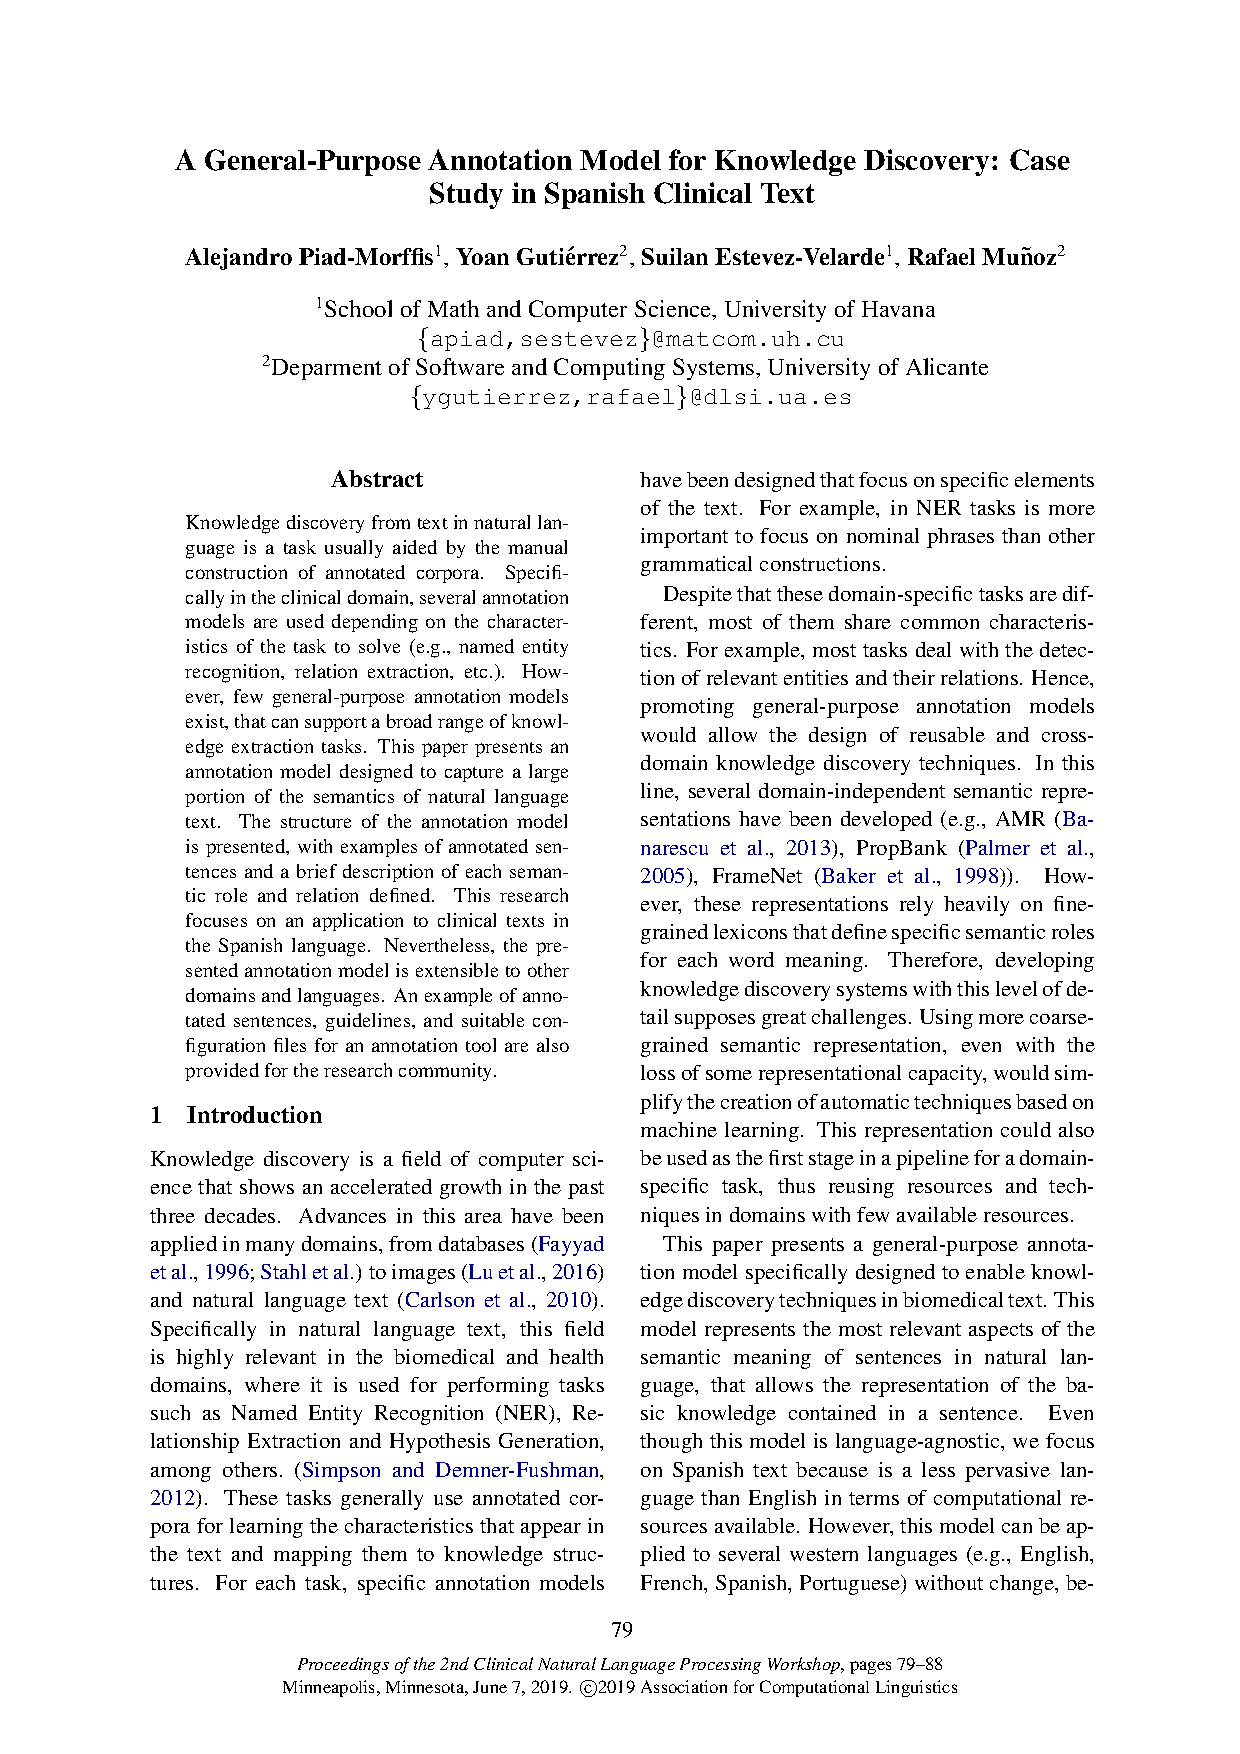
\includepdf[pages=1-, scale=0.9, offset=0 -0.75cm, pagecommand={\thispagestyle{fancy}}]{./Chapters/Papers/NAACL-Schema.pdf}

	
\chapter[Corpus eHealth-KD 20198 \textit{A corpus to support eHealth Knowledge Discovery technologies}]{Corpus eHealth-KD 2018}
\label{Chap:CorpusV1}

Ese capítulo presenta el artículo \textit{A corpus to support eHealth Knowledge Discovery technologies}.
Este artículo introduce y describe el corpus \textit{eHealth-KD 2018}. El corpus es una colección de $1173$ oraciones relacionadas con la salud en español anotadas manualmente con una estructura semántica general que captura la mayor parte del contenido, sin recurrir a etiquetas de dominio específico. La representación semántica se define e ilustra primero con oraciones de ejemplo del corpus. Se resume además el proceso de anotación y se proporcionan métricas relevantes del corpus. Finalmente, se presentan tres implementaciones computacionales, que son compatibles con los modelos de aprendizaje automático y fueron diseñadas para estimar la complejidad del aprendizaje de la semántica del corpus. El corpus resultante se utilizó como escenario de evaluación en TASS 2018 y se discuten los resultados obtenidos por los participantes. El corpus \textit{eHealth-KD} proporciona el primer paso en el diseño de un marco semántico de propósito general que se puede utilizar para extraer conocimiento de varios dominios.

\BlankLine
\noindent \textbf{Entrada bibliográfica:}\\
Piad-Morffis, A., Gutiérrez, Y., Muñoz, R. (2019). A corpus to support ehealth knowledge discovery technologies. \textit{Journal of Biomedical Informatics}, 94, 103172.

\BlankLine
\noindent \textbf{Disponible en:} \url{https://doi.org/10.1016/j.jbi.2019.103172}

    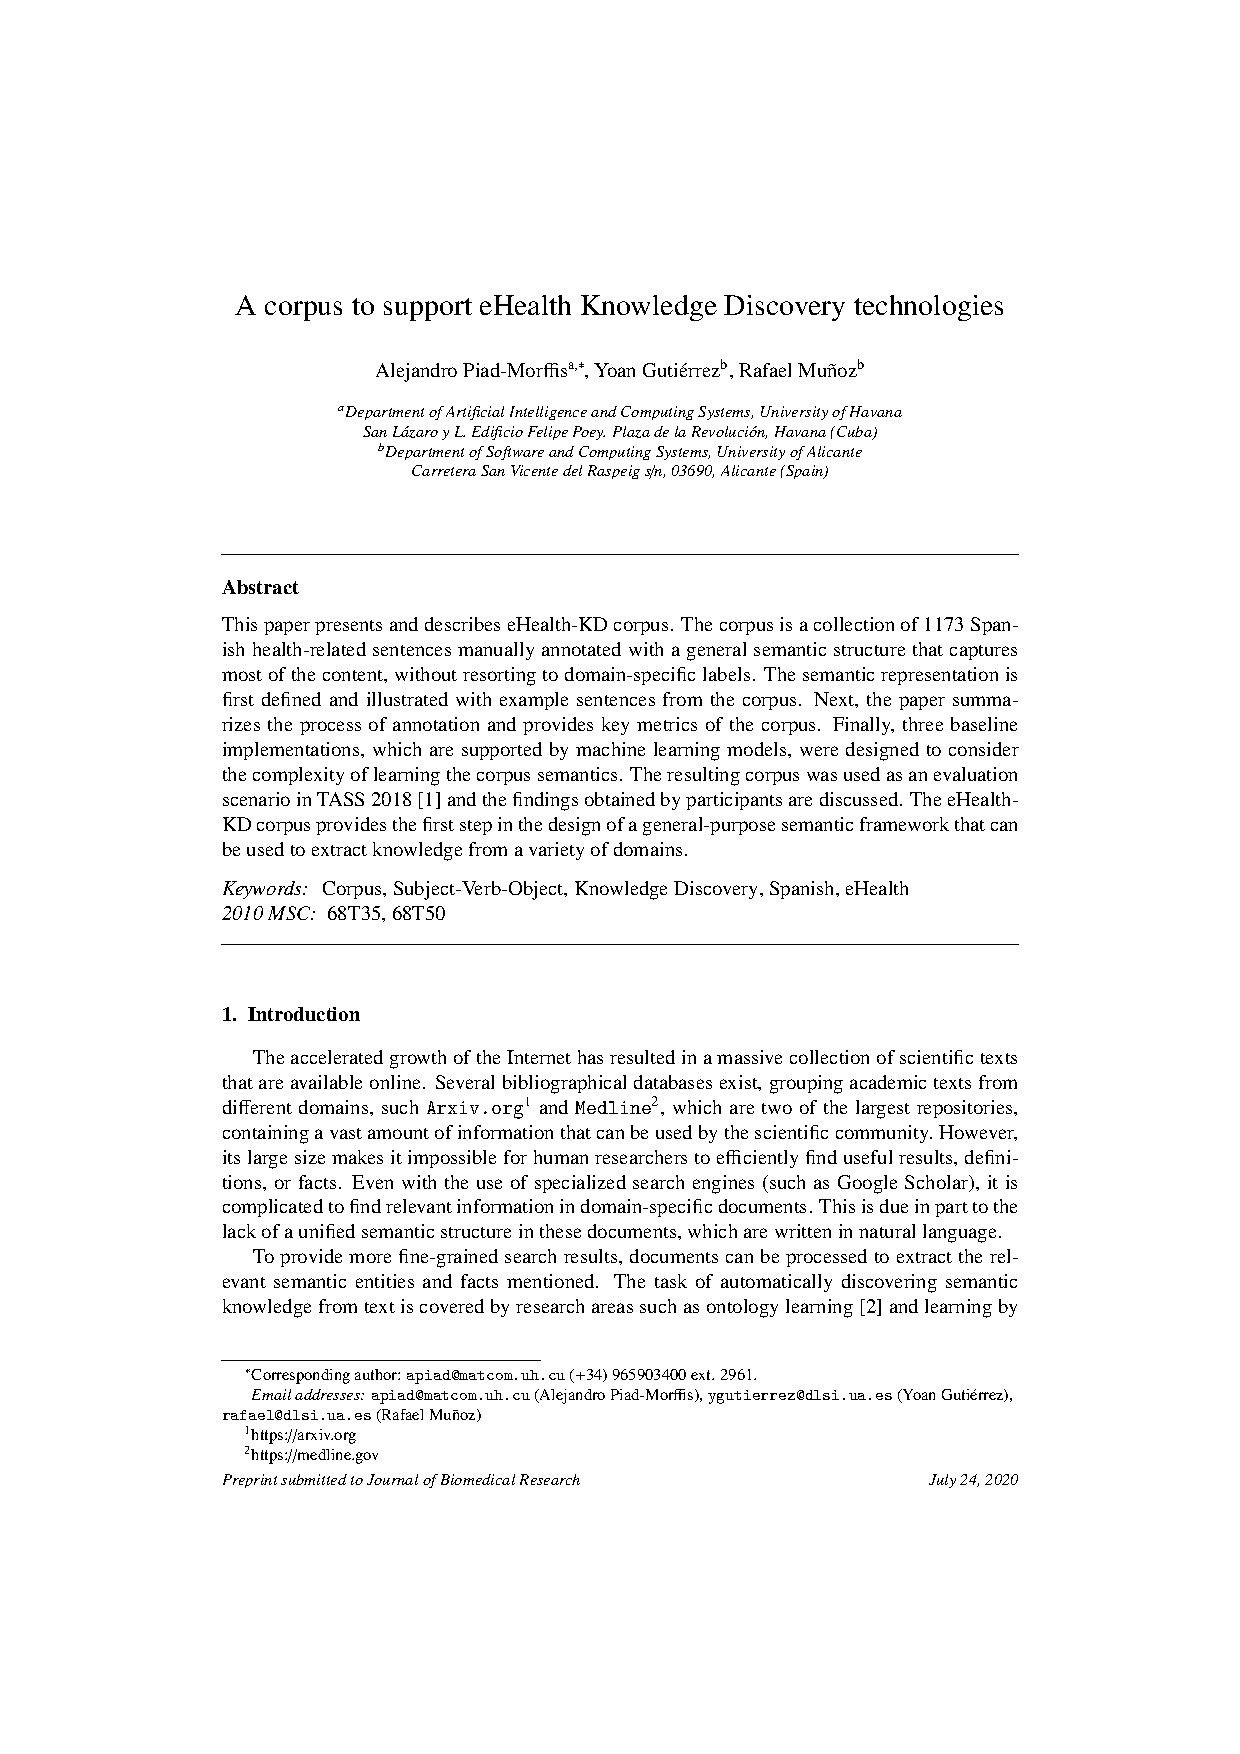
\includepdf[pages=1-, scale=1.05, offset=0 -0.75cm, pagecommand={\thispagestyle{fancy}}]{./Chapters/Papers/JBI-19.pdf}

	
\chapter[eHealth Knowledge Discovery 2018: \textit{Analysis of eHealth Knowledge Discovery Systems inthe TASS 2018 Workshop}]{eHealth Knowledge Discovery 2018}
\label{Chap:eHealthKD18}

Ese capítulo presenta el artículo \textit{Analysis of eHealth Knowledge Discovery Systems inthe TASS 2018 Workshop}.
En este artículo se analizan los sistemas presentados en la primera edición del evento \textit{eHealth Knowledge Discovery}.
Se presenta una breve descripción de la tarea, las métricas de rendimiento, y los sistemas presentados.
Además, se presenta un análisis de los resultados obtenidos por estos sistemas, enfocándose en las características de cada subtarea.
Los resultados de esta primera edición del evento demostraron que el descubrimiento de conocimiento en idioma español es un área de investigación fructífera.

\BlankLine
\noindent \textbf{Entrada bibliográfica:}\\
Alejandro Piad-Morffis, Yoan Gutiérrez, Suilan Estevez-Velarde, Yudivian Almeida-Cruz, Andrés Montoyo, and Rafael Muñoz. Analysis of eHealth Knowledge Discovery Systems in the TASS 2018 Workshop. \textit{Procesamiento del Lenguaje Natural}, 62(0):13--20, 2019. ISSN 1989-7553.

\BlankLine
\noindent \textbf{Disponible en:} \url{http://journal.sepln.org/sepln/ojs/ojs/index.php/pln/article/view/5947}.

    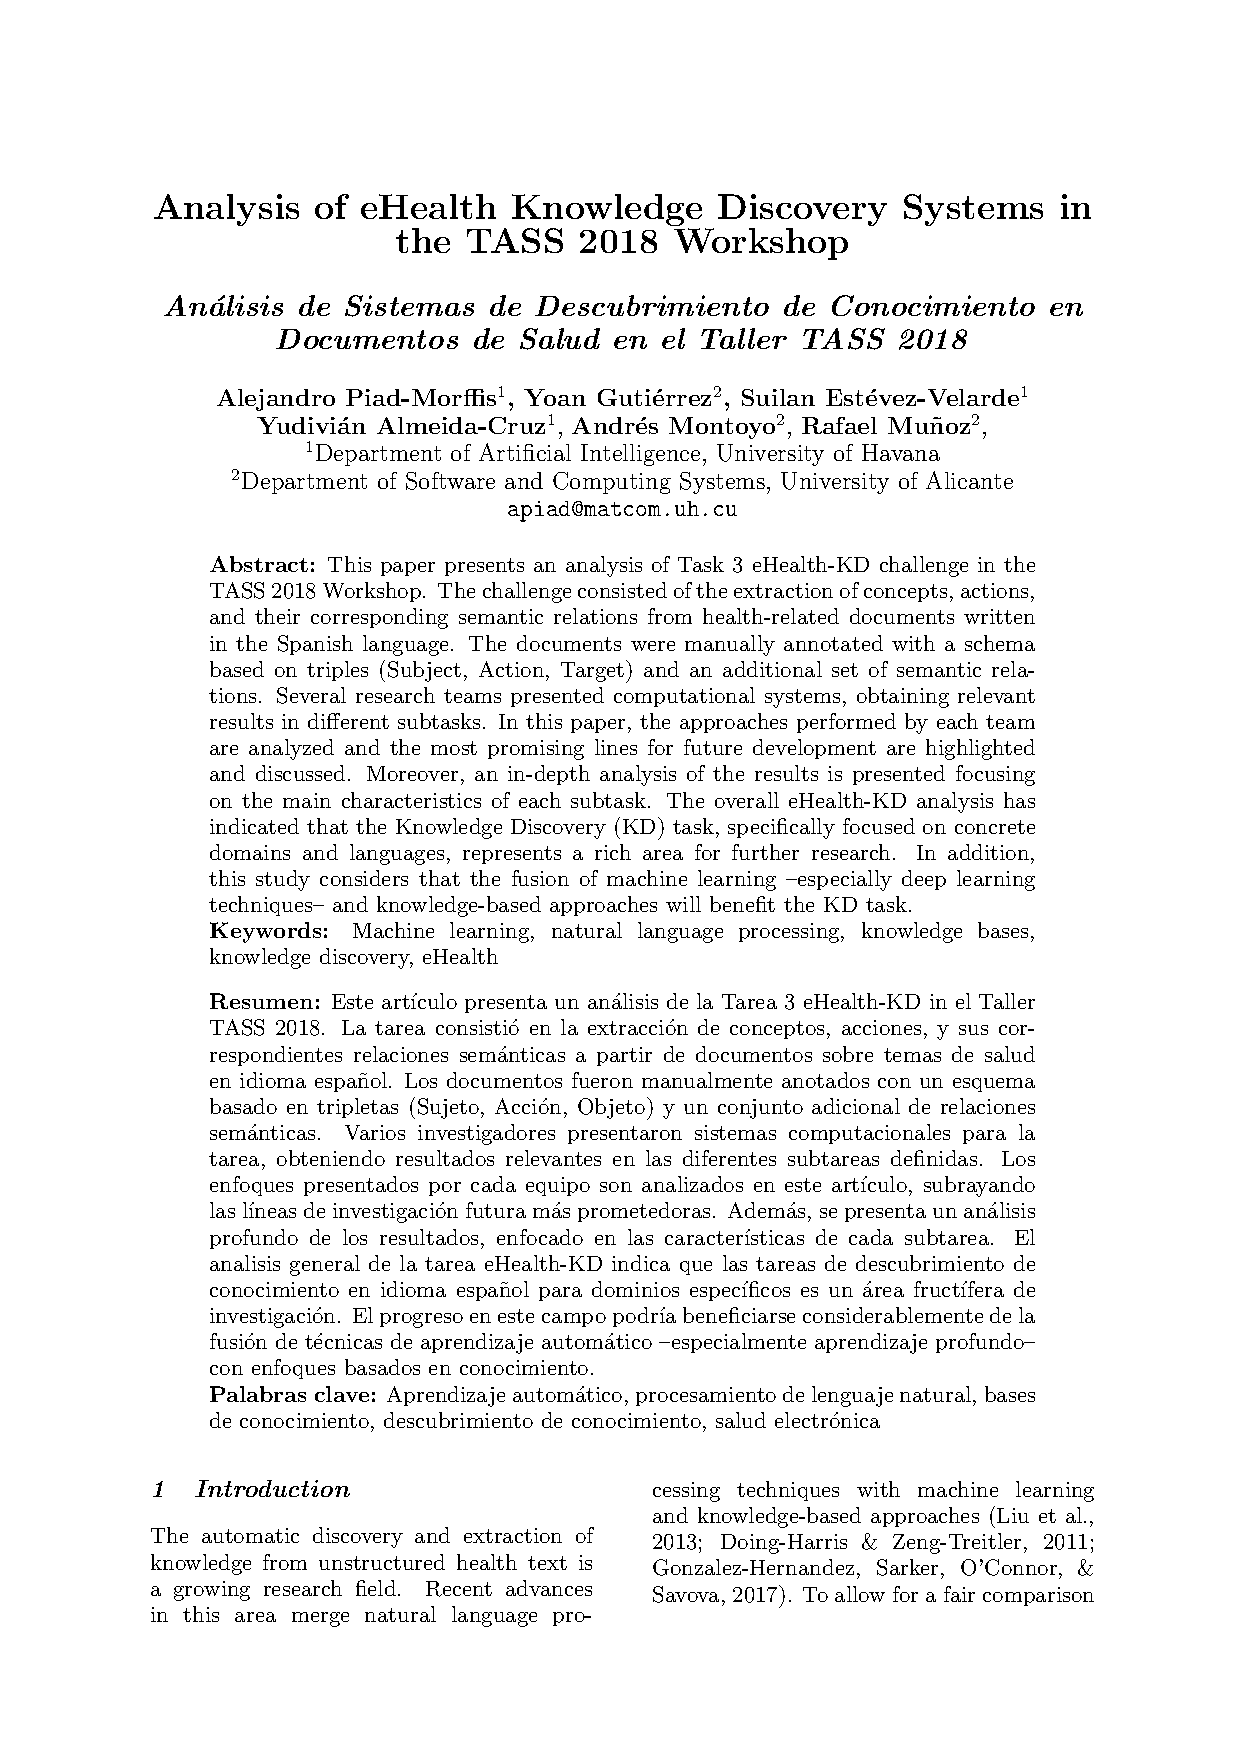
\includepdf[pages=1-, scale=0.9, offset=0 -0.75cm, pagecommand={\thispagestyle{fancy}}]{./Chapters/Papers/SEPLN-18.pdf}

	
\chapter[Ecosistema Computacional: \textit{A Computational Ecosystem to Support eHealth Knowledge Discovery Technologies in Spanish}]{Ecosistema Computacional}
\label{Chap:CorpusV2}

Este capítulo presenta el artículo \textit{A Computational Ecosystem to Support eHealth Knowledge Discovery Technologies in Spanish}. Este trabajo describe un ecosistema que facilita la investigación y el desarrollo en el descubrimiento del conocimiento en el dominio biomédico, específicamente en el idioma español. Con este fin, se desarrollan y comparten varios recursos con la comunidad de investigación, incluido un nuevo modelo de anotación semántica, un corpus anotado de 1.045 oraciones y recursos computacionales para construir y evaluar técnicas automáticas de descubrimiento de conocimiento. Además, se define una tarea de aprendizaje automático con criterios de evaluación objetivos, y se diseña un entorno de evaluación en línea, lo que permite a los investigadores interesados en esta tarea obtener resultados inmediatos y compararlos con el estado del arte. Como caso de estudio, se analizan los resultados de un evento competitivo basado en estos recursos y se brindan pautas para futuras investigaciones.

\BlankLine
\noindent \textbf{Entrada bibliográfica:}\\
Piad-Morffis, A., Gutiérrez, Y., Almeida-Cruz, Y., Muñoz, R. (2020). A computational ecosystem to support eHealth Knowledge Discovery technologies in Spanish. \textit{Journal of Biomedical Informatics}, 109, 103517.

\BlankLine
\noindent \textbf{Disponible en:} \url{https://doi.org/10.1016/j.jbi.2020.103517}

    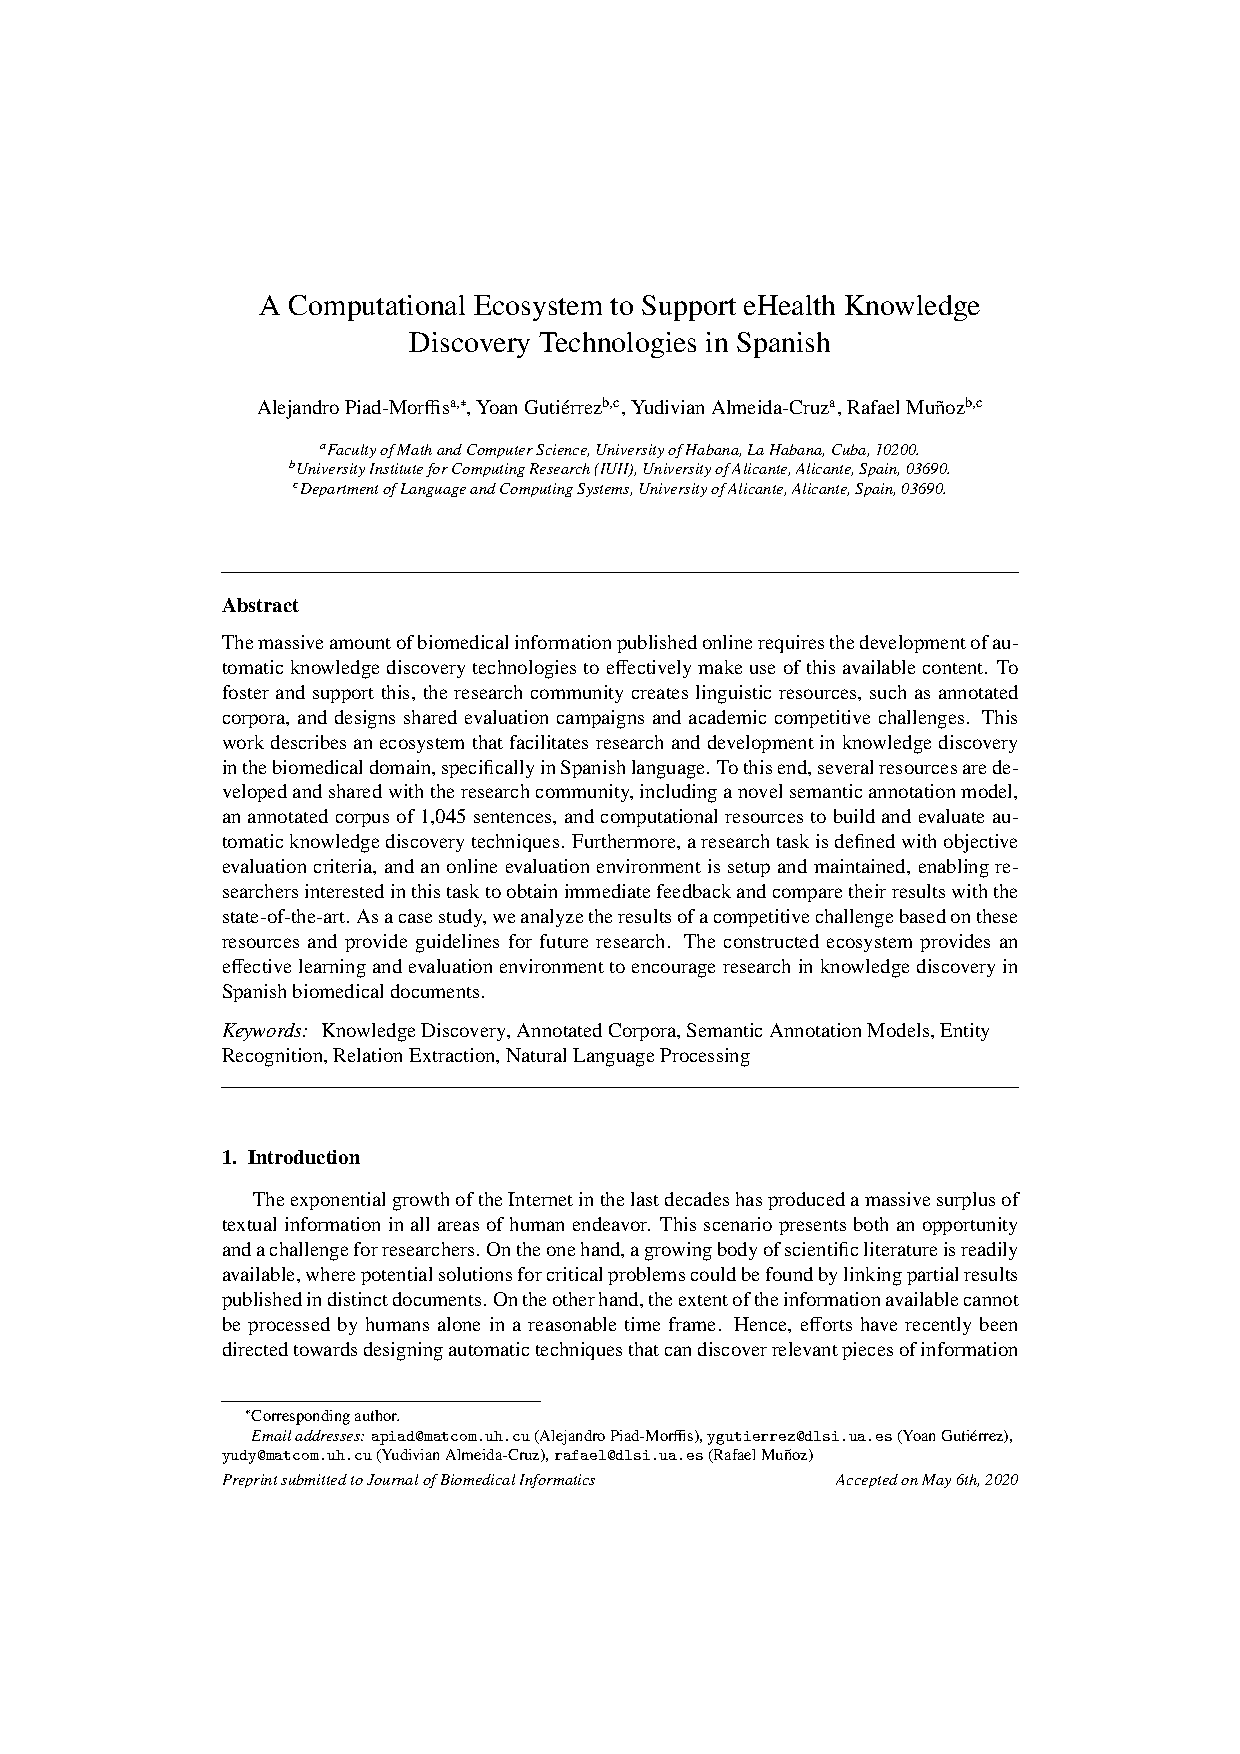
\includepdf[pages=1-, scale=1.05, offset=0 -0.75cm, pagecommand={\thispagestyle{fancy}}]{./Chapters/Papers/JBI-20.pdf}

	
\chapter[eHealth Knowledge Discovery 2021: \textit{Overview of the eHealth Knowledge DiscoveryChallenge at IberLEF 2021}]{eHealth Knowledge Discovery 2021}
\label{Chap:eHealthKD21}

Este capítulo presenta el artículo \textit{Overview of the eHealth Knowledge Discovery Challenge at IberLEF 2021}.
Este artículo resume los resultados de la última edición del evento \textit{eHealth Knowledge Discovery}.
A partir de una comparación con los resultados de ediciones anteriores, permite apreciar el avance que se ha producido en el campo en los cuatro años en los que se ha organizado el evento.
En esta edición la tarea se extendió a nuevos dominios e idiomas, lo que permitió contrastar los resultados de sistemas de dominio específico con respecto a sistemas diseñados para la generalización.
Estos resultados demuestran que la tarea de descubrimiento de conocimiento en lenguaje natural en múltiples dominios aún representa un reto científico y tecnológico relevante.

\BlankLine
\noindent \textbf{Entrada bibliográfica:}\\
Alejandro Piad-Morffis, Yoan Gutiérrez, Suilan Estevez-Velarde, Yudivian Almeida-Cruz, Andrés Montoyo, and Rafael Muñoz. Overview of the eHealth Knowledge Discovery Challenge at IberLEF 2021.\textit{Procesamiento del Lenguaje Natural}, 67(0):233--242. 2021. ISSN 1989-7553.

\BlankLine
\noindent \textbf{Disponible en:} \url{http://journal.sepln.org/sepln/ojs/ojs/index.php/pln/article/view/6392}

    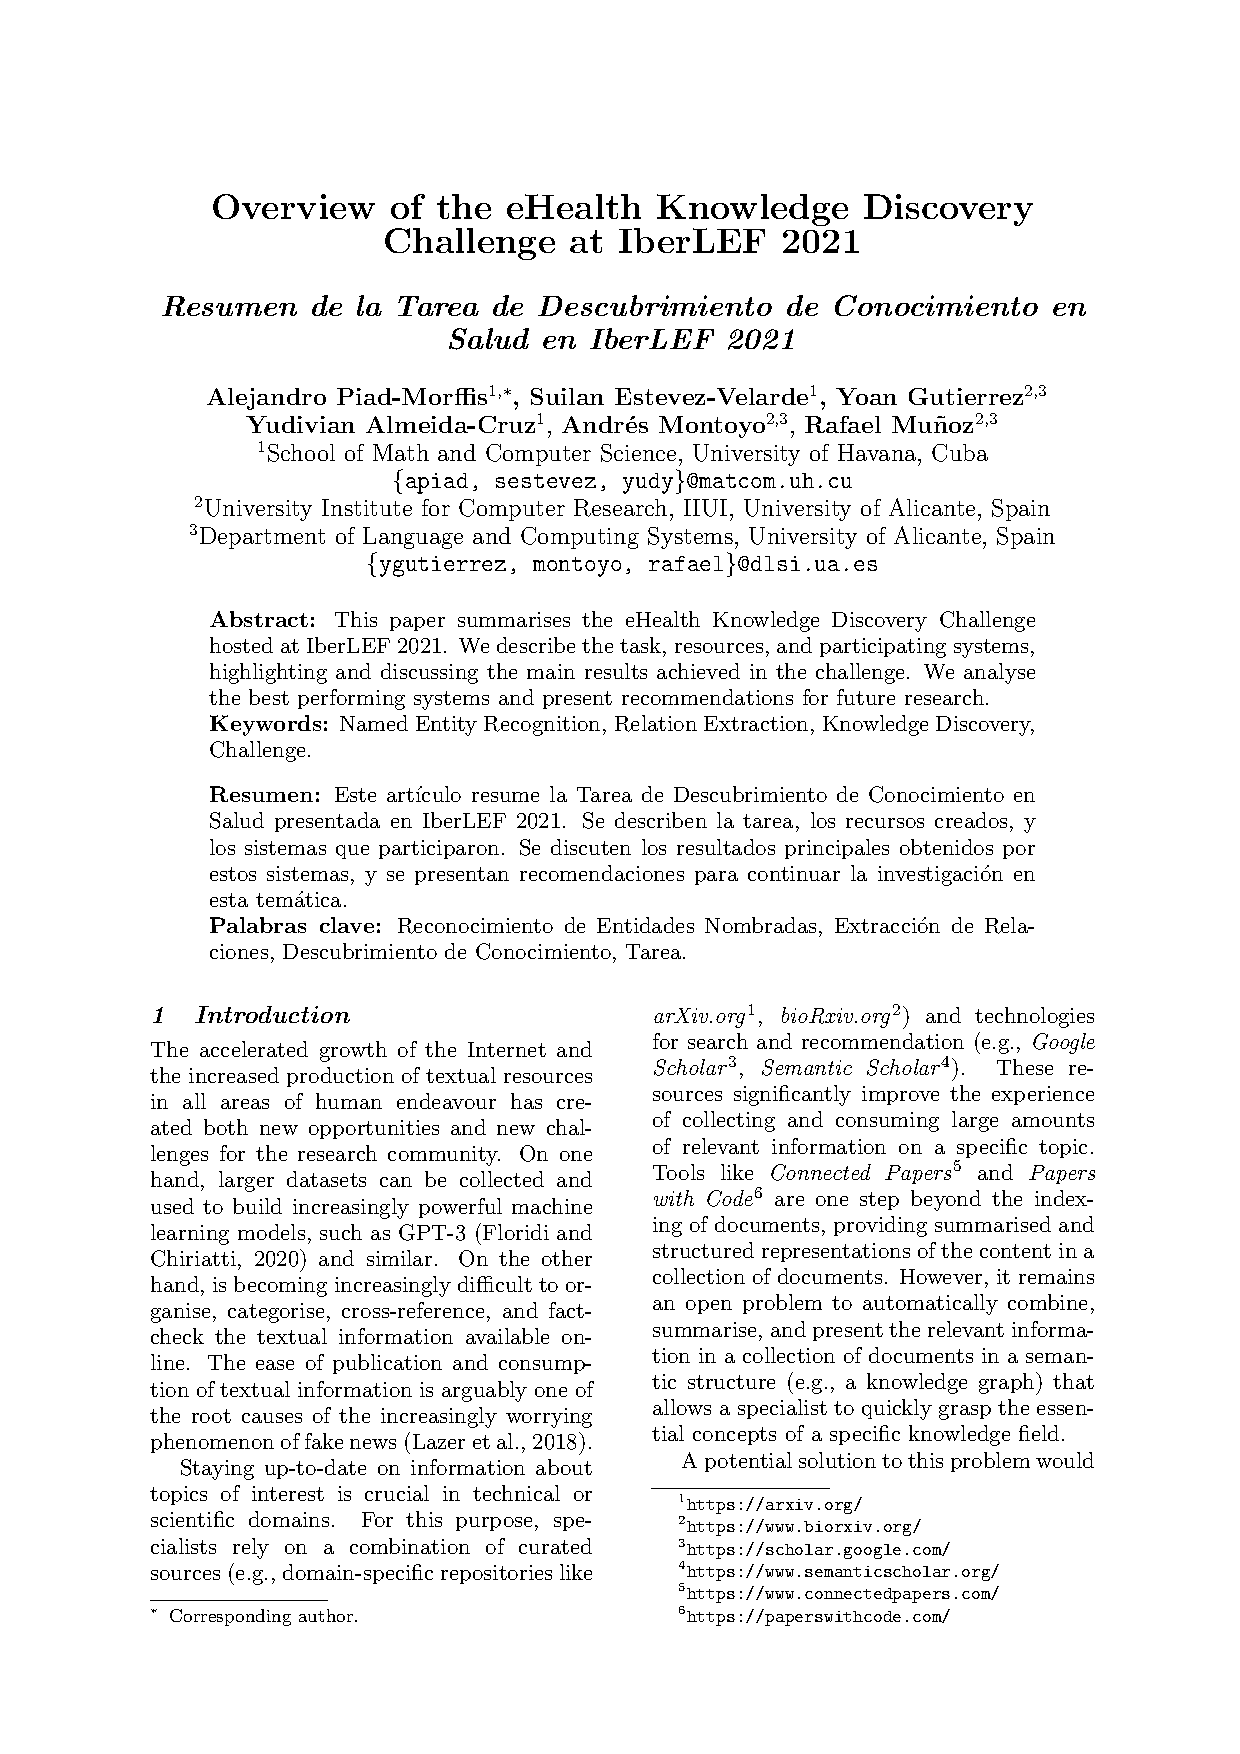
\includepdf[pages=1-, scale=0.9, offset=0 -0.75cm, pagecommand={\thispagestyle{fancy}}]{./Chapters/Papers/SEPLN-21.pdf}

    
\chapter[Anotación Asistida: \textit{Active Learning for Assisted Corpus Construction:A Case Study in Knowledge Discovery from Biomedical Text}]{Anotación Asistida}
\label{Chap:Annotation}

Este capítulo presenta el artículo \textit{Active Learning for Assisted Corpus Construction:A Case Study in Knowledge Discovery from Biomedical Text}.
Este artículo define un enfoque de aprendizaje activo que tiene como objetivo reducir el esfuerzo humano requerido durante la anotación de corpus en lenguaje natural, compuestos por entidades y relaciones semánticas. Nuestro enfoque ayuda a los anotadores humanos seleccionando inteligentemente las oraciones más informativas para anotar y pre-anotándolas con algunas entidades y relaciones semánticas. Se define una estrategia basada en la incertidumbre con un factor de densidad ponderado, utilizando métricas de similitud basadas en \textit{embeddings} de oraciones. Los resultados experimentales sugieren que la estrategia de consulta reduce entre un $35\%$ y $40\%$ el número de oraciones que se deben anotar manualmente para desarrollar sistemas capaces de alcanzar un resultado objetivo de $F_1$,
mientras que la estrategia de pre-anotación produce una reducción adicional de $24\%$ en el tiempo total de anotación.

\BlankLine
\noindent \textbf{Entrada bibliográfica:}\\
Hian Cañizares-Díaz, Alejandro Piad-Morffis, Suilan Estevez-Velarde, Yoan Gutiérrez, Yudivián
Almeida Cruz, Andrés Montoyo and Rafael Muñoz-Guillena. Active Learning for Assisted Corpus Construction: A Case Study in Knowledge Discovery from Biomedical Text. \textit{Proceedings of RANLP 2021.}

\BlankLine
\noindent \textbf{Disponible en:} \url{https://ranlp.org/ranlp2021/proceedings-20Sep.pdf}

    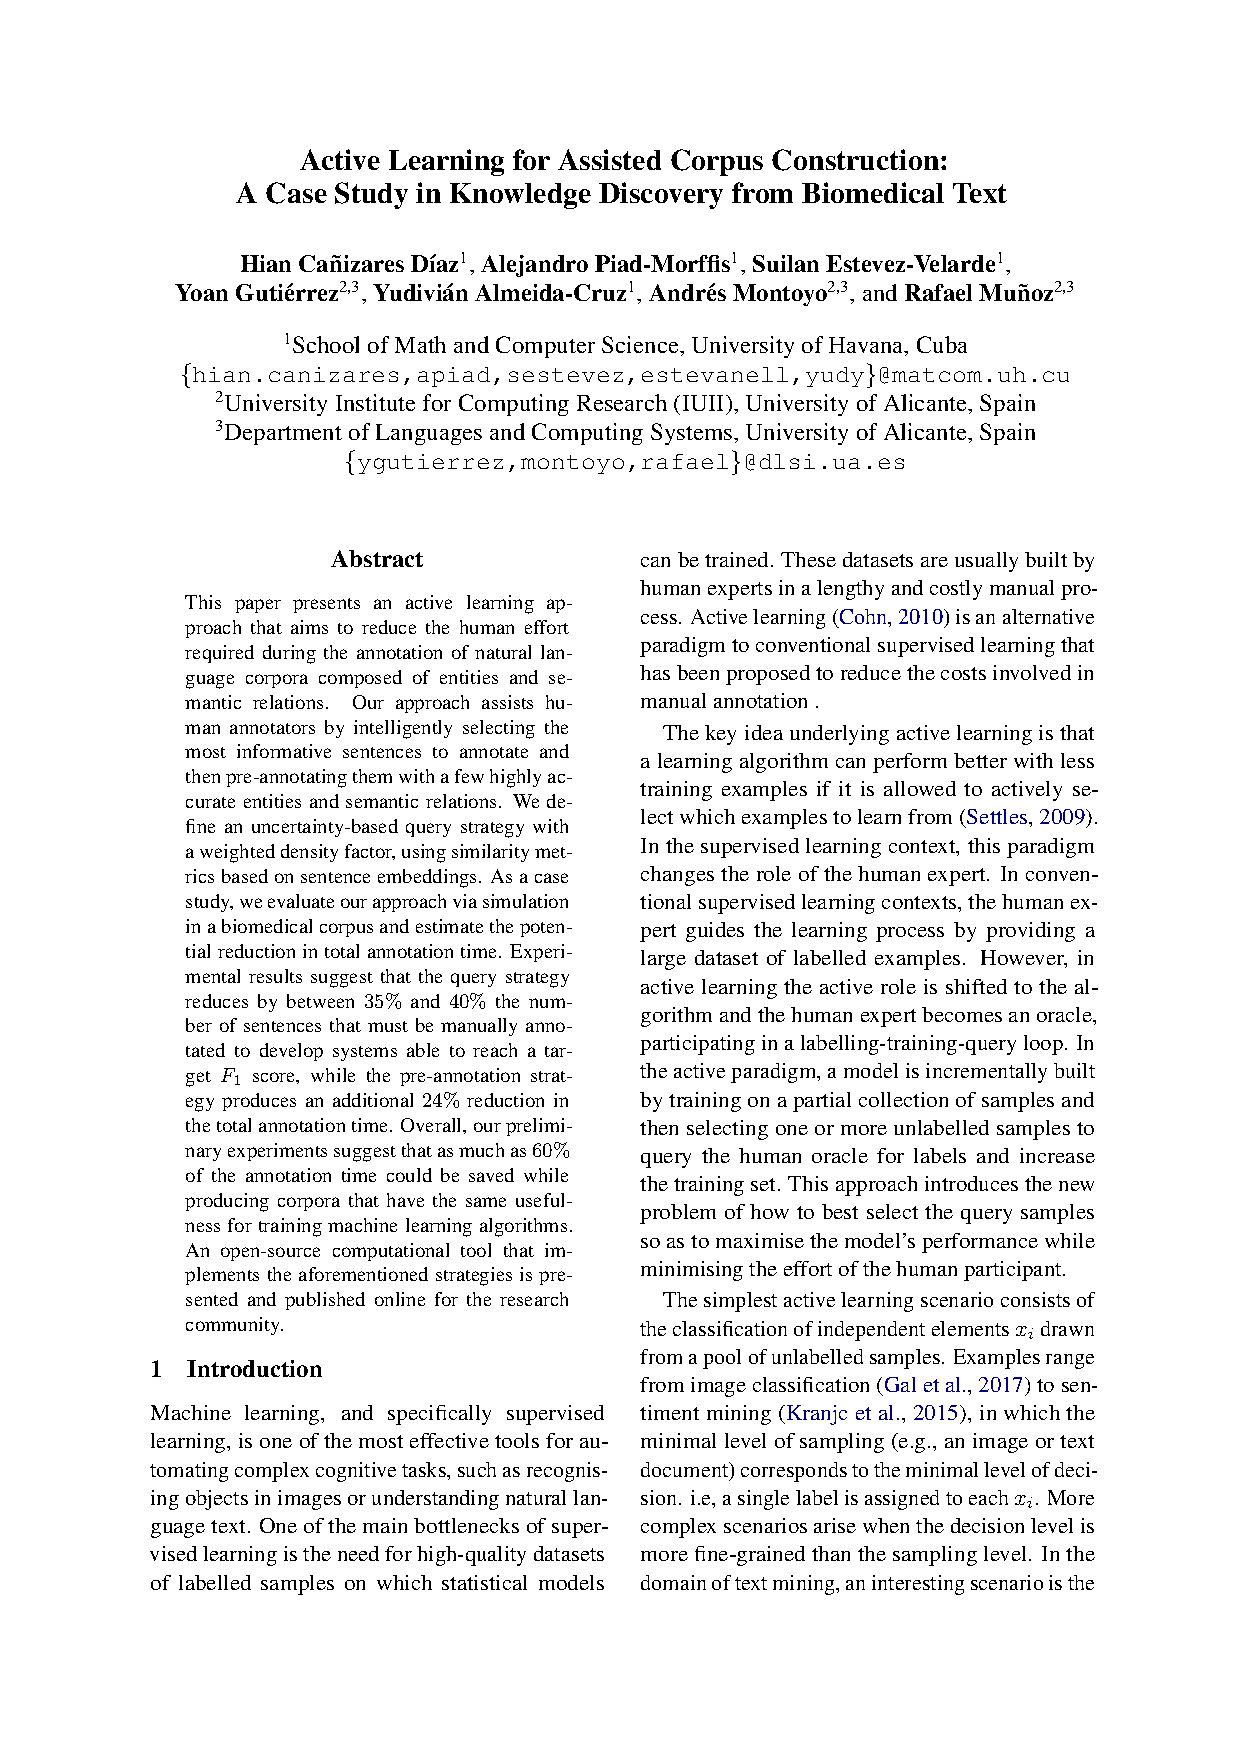
\includepdf[pages=1-, scale=0.9, offset=0 -0.75cm, pagecommand={\thispagestyle{fancy}}]{./Chapters/Papers/RANLP-ActiveLearning.pdf}

%%TC:endignore

    \part{Conclusiones y Recomendaciones}

    \pagestyle{fancyNormalChapterStyle}	% - Fixing style for the regular chapters

    %   <Conclusions>   %
    \chapter{Conclusiones}\label{Chap:Conclusions}
\markboth{\MakeUppercase{Conclusiones}}{}

El volumen de información que se publica cada día es una fuente de conocimiento relevante de gran utilidad para la comunidad científica. A partir del análisis de múltiples fuentes es posible encontrar conexiones que permitan potencialmente descubrir nuevo conocimiento que se encuentra disperso en las redes.
A pesar de esto, el alto número de fuentes a revisar es imposible de procesar por humanos, lo que dificulta este proceso de descubrimiento de conocimiento.
En este contexto cobra especial relevancia el desarrollo de técnicas automáticas para la extracción y descubrimiento de este conocimiento.

El dominio de la salud es uno de los que más puede beneficiarse del descubrimiento automático de conocimiento, debido a la velocidad y el volumen con el que se publican nuevos resultados. La reciente pandemia de COVID-19 es solo un ejemplo más de la necesidad de conectar de forma automática los hechos y resultados publicados a diario. Para construir sistemas computacionales capaces de realizar esta tarea, es necesario no solo la creación de recursos lingüísticos que sirvan para los modelos de aprendizaje automático, sino también la creación de una infraestructura que permita a los investigadores evaluar sus sistemas de forma efectiva y compararlos con el estado del arte.

Esta investigación presenta el diseño y la construcción de un ecosistema para el desarrollo de tecnologías de descubrimiento de conocimiento, enfocado en el dominio de la salud y el idioma español.
Este ecosistema incluye recursos lingüísticos, herramientas computacionales y una metodología para la evaluación de nuevos enfoques.

Con el objetivo de representar de forma computacionalmente manejable el lenguaje natural, se definió un modelo de anotación para capturar el contenido semántico más relevante de una oración, basado en una estructura Sujeto-Acción-Objetivo y relaciones semánticas adicionales.
El modelo no incluye entidades o relaciones de dominio específico para ser lo más general posible. Este modelo está diseñado para ser suficientemente expresivo pero que aún así sea factible tanto su anotación por expertos humanos con un alto grado de acuerdo entre diferentes anotadores como la aplicación de técnicas de aprendizaje automático.

Basado en este esquema de anotación, se anotaron manualmente a lo largo de la investigación cuatro versiones de un corpus con un total de $41,163$ elementos semánticos repartidos en $3,068$ oraciones, tomando como base información en el dominio de salud en idioma español. A pesar del enfoque en el dominio de la salud, a modo de caso de estudio se incluyen $300$ oraciones en un dominio alternativo (reportajes periodísticos), $200$ oraciones en idioma inglés, que demuestran la capacidad de generalización del esquema de anotación. Los cuatro versiones de un corpus fueron anotados por equipos compuestos por anotadores expertos y no expertos, siguiendo un protocolo que garantizó un alto grado de acuerdo en los elementos anotados.
El propósito de estos recursos lingüísticos es permitir la creación de sistemas de descubrimiento de conocimiento a partir del uso de técnicas de aprendizaje automático.
Con este propósito, se ha organizado una campaña de evaluación, \textit{eHealth-KD challenge}, de la que se han producido cuatro ediciones consecutivas. En total han participado un total de $33$ equipos de investigadores de diferentes nacionalidades con múltiples estrategias, principalmente enfocadas en arquitecturas de aprendizaje profundo. Para permitir una comparación entre diferentes sistemas, se diseñó un escenario que consiste de dos subtareas fundamentales, y se definieron un conjunto de métricas para su evaluación.
Los resultados obtenidos en las cuatro ediciones de esta campaña demuestran que el reto de descubrir conocimiento automáticamente en lenguaje natural es un problema aún abierto pero se ha producido una mejora considerable en la efectividad de los sistemas presentados de una edición a la siguiente, fomentado por el reciente desarrollo de nuevas arquitecturas de aprendizaje profundo para el procesamiento de lenguaje natural.

Más allá de las ediciones de la campaña \textit{eHealth-KD}, esta investigación se propuso construir un ecosistema de evaluación continua que pueda ser utilizado de forma independiente por cualquier investigador para evaluar nuevos enfoques y compararse con el estado del arte.
Este ecosistema se pone a disposición de la comunidad científica, que consiste una infraestructura y un conjunto de herramientas (incluyendo implementaciones básicas con las que compararse), un entorno de evaluación continua en la nube, y estadísticas actualizadas sobre el estado del arte de la tarea \textit{eHealth-KD}.
Todos estos recursos, incluyendo los corpus anotados y las herramientas computacionales están publicados bajo licencias de código abiertas y disponibles para su uso en línea\footnote{\url{https://ehealthkd.github.io}}.

Finalmente, a partir de las experiencias acumuladas durante el proceso de anotación, se implementó un sistema de anotación asistida que permite reducir considerablemente el costo manual de producir nuevos recursos lingüísticos en esta área.
Este sistema utiliza técnicas de aprendizaje automático para seleccionar las oraciones más útiles a anotar, y garantizar un balance de los datos en un corpus con el menor esfuerzo posible por parte de los anotadores humanos.
Esta herramienta está basada en componentes de código abierto y se encuentra disponible para el uso de la comunidad científica\footnote{\url{https://github.com/knowledge-learning/assisted-annotation}}.

Todos los resultados presentados en esta Tesis son parte de una línea de investigación activa para aprovechar la semántica de propósito general y las tecnologías basadas en el conocimiento junto con las nuevas arquitecturas de aprendizaje profundo en la construcción de tecnologías automáticas de descubrimiento de conocimiento.
Como parte de esta línea, se continúa trabajando en la expansión de los recursos lingüísticos creados y en la organización de campañas de evaluación para fomentar la investigación en esta temática en la comunidad, así como en el desarrollo de nuevas herramientas computacionales basadas en técnicas de aprendizaje automático para el descubrimiento de conocimiento a partir de lenguaje natural.

\section{Publicaciones}
\label{Chap:Conclusions-Publications}

Los resultados de investigación parciales que conforman esta tesis se han publicado anteriormente en diversos artículos. A continuación se listan aquellas publicaciones relacionadas con esta investigación en las que ha participado el autor:

\begin{itemize}
    \item Overview of TASS 2018: Opinions, health and emotions~\cite{tamartinez2018overview}
    \item Overview of the eHealth Knowledge Discovery Challenge at IberLEF 2019~\cite{tapiad2019overview}
    \item Overview of the eHealth Knowledge Discovery Challenge at IberLEF 2020~\cite{piad2020overview}
    \item Overview of the eHealth Knowledge Discovery Challenge at IberLEF 2021~\cite{piad2021overview}
    \item A general-purpose annotation model for knowledge discovery: Case study in Spanish clinical text~\cite{tapiad2019general}
    \item A corpus to support eHealth Knowledge Discovery technologies~\cite{piad2019corpus}
    \item A Computational Ecosystem to Support eHealth Knowledge Discovery Technologies in Spanish~\cite{piad2020computational}
    \item Gathering object interactions as semantic knowledge~\cite{taestevez2018gathering}
    \item TASS 2018: The strength of deep learning in language understanding tasks~\cite{tass}
    \item A Neural Network Component for Knowledge-Based Semantic Representations of Text~\cite{tapiad2019neural}
    \item Analysis of eHealth knowledge discovery systems in the TASS 2018 workshop~\cite{taalejandro2019analysis}
    \item Active Learning for Assisted Corpus Construction:A Case Study in Knowledge Discovery from Biomedical Text~\cite{canizares2021active}
    \item Knowledge Discovery in COVID-19 Research Literature~\cite{estevanell2021knowledge}
\end{itemize}

Adicionalmente, se listan a continuación las ediciones del evento \textit{eHealth Knowledge Discovery} organizadas como parte del marco de evaluación de esta investigación:

\begin{itemize}
    \item eHealth KD 2018 como Workshop en el evento TASS 2018\\ \url{http://www.sepln.org/workshops/tass/2018/task-3}
    \item eHealth KD 2019 como Workshop en el evento IBERLEF 2019\\ \url{https://knowledge-learning.github.io/ehealthkd-2019}
    \item eHealth KD 2020 como Workshop en el evento IBERLEF 2020\\ \url{https://knowledge-learning.github.io/ehealthkd-2020}
    \item eHealth KD 2021 como Workshop en el evento IBERLEF 2021\\ \url{https://ehealthkd.github.io/2021}
\end{itemize}


    \chapter{Trabajo Futuro}\label{Chap:FutureWork}
\markboth{\MakeUppercase{Trabajo Futuro}}{}

La investigación desarrollada en esta tesis puede ser continuada desde múltiples perspectivas.
En primer lugar, los modelos teóricos de representación del conocimiento diseñados así como los algoritmos presentados, pueden ser mejorados y adaptados a nuevos escenarios.
Por otro lado, el ecosistema diseñado permite continuar con la organización de eventos competitivos en diferentes tareas y dominios para incentivar el desarrollo de nuevas técnicas de descubrimiento de conocimiento.
En este capítulo se presentan las ideas que consideramos más relevantes y que pueden proveer un mayor aporte a los resultados y aplicaciones futuras de esta investigación.

Desde la arista de desarrollo y creación de corpus, una de las líneas de investigación más claras es la anotación de nuevos recursos lingüísticos en otros dominios e idiomas. 
Entre los dominios más interesantes a analizar se encuentran los artículos científicos, las noticias y los artículos enciclopédicos. Estas son fuentes de información factual que presentan diferentes características sintácticas pero que potencialmente pueden ser capturadas con las mismas estructuras semánticas definidas en esta investigación.
Anotar nuevos dominios permitiría también ampliar el \textit{eHealth-KD} a una audiencia mayor, por ejemplo, los investigadores interesados en el fenómeno de las noticias falsas.
Además, esto abre las puertas a la definición de tareas multi-dominio, donde los mismos sistemas sean evaluados en corpus de dominios diferentes a los que fueron entrenados, requiriendo el desarrollo de técnicas de transferencia de aprendizaje automático.

En la dirección de modernizar la tarea \textit{eHealth-KD} hay dos escenarios nuevos interesantes de explorar.
En primer lugar, adicionar el problema de reconocimiento de los atributos, que actualmente son anotados en el corpus pero no evaluados en la tarea. Este escenario ya introduce algunos problemas computacionales interesantes, por ejemplo, la identificación de la negación y su ámbito.
Con vistas a avanzar hacia una representación semántica de más alto nivel, el otro escenario de interés consiste en la normalización de las entidades extraídas en función de bases de datos estructuradas, por ejemplo, Wikidata.
Estas adiciones complejizan la tarea \textit{eHealth-KD}, pero como mismo se separan la extracción de entidades y relaciones en diferentes subtareas, se pueden definir subtareas específicas para estos problemas permitiendo que investigadores especializados en un área participen en aquellos problemas de su interés.

El esquema de anotación propuesto en esta investigación ha demostrado ser capaz de capturar una porción significativa de la semántica del lenguaje natural. Sin embargo, aún mantiene algunas inconsistencias y ambigüedades que pueden ser mejoradas con pocas modificaciones. 
Una de las principales fuentes de ambigüedad identificada es la similitud entre los roles de \texttt{Predicate} y la relación \texttt{in-context}. Es posible que una de estas variantes sea redundante, o que deba definirse de manera más clara la diferencia entre ambos patrones de anotación.
La adición más importante al esquema de anotación consistiría en un nuevo tipo de relación semántica que permita denotar el propósito de una acción o evento.

Finalmente, la estrategia de aprendizaje activo desarrollada en la investigación brinda una solución prometedora al problema del costo de la anotación manual, pero solo ha sido evaluada en escenarios simulados.
La propuesta más relevante en este sentido consiste en aplicar esta estrategia para la anotación de los recursos lingüísticos de la próxima edición del \textit{eHealth-KD}.
Para esto es necesario adaptar la propuesta a un escenario con múltiples anotadores por cada oración.
En este escenario, el propio desacuerdo entre los anotadores introduce una nueva fuente de incertidumbre que puede ser utilizada para optimizar el proceso de anotación.

Las ideas sugeridas en este capítulo son solo algunas de las posibilidades más claras para continuar el desarrollo de las técnicas y recursos propuestos en esta tesis. El trabajo desarrollado forma parte de una línea de investigación activa. Estas y otras ideas serán tenidas en cuenta para estimular aún más el desarrollo de tecnologías de descubrimiento de conocimiento, siempre desde la perspectiva de aprovechar el esfuerzo humano y los recursos computacionales en estrecha colaboración. Visualizamos un futuro donde los seres humanos y las computadoras trabajen juntos en la solución de los problemas más apremiantes, cada uno poniendo sus mejores habilidades al servicio de las futuras generaciones.


	%	<Conclusions-FutureWork>	%
	%\include{./Chapters/Conclusions-FutureWork/Conclusions-FutureWork}

	%	<Part : Appendix>	%
% 	\appendix

% 	\pagestyle{fancyAppendixStyle}	% - Fixing style for the appendices

% 	%   <Annotation Guidelines> %
% 	\include{./Chapters/Annotation-Guidelines/Annotation-Guidelines}

% 	%	<Summary-Spanish>	%
% 	\include{./Chapters/Summary-Spanish/Summary-Spanish}

	\backmatter

	%	<Bibliography>	%
	\pagestyle{fancyUnnumberedSectionsStyle}	% - Fixing style for the regular chapters

    \bibliographystyle{unsrtnat}
	\bibliography{./Bibliography/Bibliography}


	%	<Nomenclature>	% (omitted for the moment)
	%I want $\beta$\nomenclature{$\beta$}{The second letter of the greek alphabet} to be listed after $\alpha$\nomenclature{$\alpha$}{The first letter of the greek alphabet} % Only to try...

	%\printnomenclature

\end{document}
